\chapter{CO\texorpdfstring{$_2$}{} reduction on MXene supported copper tetramers: The role of cluster morphology }\label{appendix3}

%%%%%%%%%%%%%%%%%%%%%%%%%%%%%%%%%%%%%%%%%%%%%%%%%%%%%%%%

\section{Introduction}
With the advent of industrial revolution in the 18th century, the need for energy has continuously increased and so has the deterioration of the climate. Exploiting fossil fuels (oil, coal and natural gas) meets the maximum portion of our energy demands\cite{leung2014overview} whereas a very small fraction is generated from renewable sources like hydro, solar and nuclear power. The extensive use of fossil fuels has not only depleted the natural reserves but has also increased the emission of harmful greenhouse gases responsible for global warming. Carbon dioxide (CO$_2$) is one of the greenhouse gases released during the combustion of fossil fuels. The increase in the level of CO$_2$ in the atmosphere has disturbed many ecological systems\cite{climate,cc}. In order to mitigate the damage CO$_2$ sequestration and storage (CSS) gained popularity. However, CO$_2$ as feed stock has no value and hence carbon capture and recycling (CCR) process started replacing CSS\cite{peters2009co,aresta2010carbon, aresta2007utilisation, centi2009opportunities} as the solution to our problems. In the ambit of CCR, CO$_2$ has been converted to many value added chemicals like methanol, ethanol, formaldehyde, formic acid and other olefins. Among the many important chemicals, methanol has the maximum versatility, as it can be used as a transportation fuel, organic feedstocks, precursor to olefins and aromatics and also be used directly as methanol fuel cells (DMFC) which converts the chemical energy in methanol to electrical energy\cite{mcgrath2004direct, lee1989methanol, ma2009short, liu2003recent, song2006global}. CO$_2$ can be obtained from the flue gases released by power plants or, directly trapped from the atmosphere\cite{peters2011chemical,goeppert2012air}. The reducing agent, hydrogen (H$_2$), is nowadays obtained from electrolysis of water using renewable energy source\cite{olah2013towards}. 

The formation of methanol from CO$_2$ and H$_2$ is an exothermic process (CO$_{2}$ + 3H$_{2}$  $\rightarrow$ CH$_{3}$OH + H$_{2}$O). However, catalysts are needed to expedite the reduction process. Among the variety of catalysts, heterogeneous thermo-catalysis on copper based catalysts (Cu/ZnO/Al$_2$O$_3$) is commercially used to reduce CO$_2$\cite{gallucci2004experimental}. CO$_2$ reduction is generally achieved in two ways. First, reduction to CO (CO + H$_2$O) via the Reverse Water Gas Shift (r-WGS) reaction and then further hydrogenate CO as syn gas (CO + CO$_2$ + H$_2$O) to methanol and other value added chemicals\cite{lee2014handbook,goehna1994producing}. Second, direct reduction to methanol\cite{rodemerck2013catalyst}. The formation of methanol industrially is accompanied by the formation of water which is responsible for the sintering of Cu and ZnO and eventual deactivation of the catalyst. Moreover, incomplete reduction of CO$_2$ along with the formation of trace by-products like esters, hydrocarbons, C2+ alcohols etc. increases the cost of distillation. Therefore, the catalytic performance of industrial catalysts are not optimum and can be improved. 

Zhang et al.\cite{zhang2018optimum} have predicted copper nanoclusters to possess better catalytic activity than extended Cu surfaces (Cu(111), Cu(211)). Most recently\cite{behrens2012active,tao2019best,posada2016conversion,yang2010fundamental}, at the laboratory scale, supported nanoclusters of Cu has been used to reduce CO$_2$ to single carbon products like methanol, carbon monoxide, formic acid and formaldehyde. Yang et al.\cite{yang2017copper} finds the tetramer cluster supported on Al$_2$O$_3$ (Cu$_4$/Al$_2$O$_3$) to show better catalytic conversion than Cu$_3$/Al$_2$O$_3$ and Cu$_{20}$/Al$_2$O$_3$. In the preparation of the supported nanoclusters, a size-selected source enabled by single mass selection is used to soft land the metal cluster on the support\cite{yin2014atomically,lu2014effect}. The process guarantees the deposition of a particular size of the cluster but the shape and geometry of the cluster is dependent on the interaction amongst cluster atoms and between cluster and support. Hence, it intrigues us to look into the role of geometry in the CO$_2$ reduction process. As a model system, we compared the CO$_2$ reduction (hydrogenation) process on the rhombus and tetrahedral geometries of copper tetramer supported on O-terminated MXene (Ti$_2$CO$_2$).   

The remainder of this chapter is divided into four sections. Section II describes the computational methods undertaken. Additional details regarding the energy of the reaction processes is also discussed. Section III lays down the results along with their discussions obtained from this study. This section has four subsections. First describes the different pathways for the reduction of CO$_2$. Second and third reports the reaction profile of CO$_2$ reduction on the MXene supported rhombus and tetrahedral tetramers respectively. Fourth subsection compares the reaction profile of the two catalysts and rationalizes the observations. Finally, the overall work in concluded in Section IV. 

\section{Computational details }
\label{compdettt}

Quantum ESPRESSO (QE) software\cite{QE2009}, a plane wave based implementation of density functional theory, was used to perform spin polarised calculations. The electronic exchange and correlation are energies parameterized by Perdew, Burke and Ernzerhof (PBE)\cite{GGA-PBE1996} within the generalized gradient approximation (GGA) framework. Since van der Waals interactions are important for these systems and conventional PBE functionals do not include them, we have incorporated Grimme's semiempirical corrections\cite{grimme2006semiempirical} in our calculations. The electron-ion interactions were described by ultrasoft pseudopotentials\cite{USPP1990}. For each of the elements, pseudopotentials with the following valence configurations were used: (a) Ti : [3$s{^2}$, 3$p{^6}$, 3$d{^2}$, 4$s{^2}$], (b) Cu : [3$d^{10}$, 4$s{^1}$], (c) O : [2$s{^2}$, 2$p{^4}$], (d) C :[2$s{^2}$, 2$p{^2}$], and (e) H : [1$s^1$]. The expansion of wave function and charge density were done using a plane wave basis with kinetic energy cutoffs of 55 Ry and 480 Ry respectively. Brillouin zone (BZ) integrations of the (1 $\times$ 1) unit cell of the substrate (Ti$_2$CO$_2$) were performed using a 12 $\times$ 12 $\times$ 1 shifted Monkhorst-Pack k-point mesh\cite{K-pointMP1976}, whereas for the molecules in the gas phase BZ integrations were done using the $\Gamma$-point only. In order to converge the electronic energy faster, Marzari-Vanderbilt smearing\cite{SmearingMV1999} with width of 0.007 Ry was used. 

In this work, the catalysts are tetramer clusters (rhombus and tetrahedron) deposited on 2D O-terminated Ti$_2$C MXene. The products of the CO$_2$ hydrogenation are stable gas phase molecules like formic acid, formaldehyde, methanol and carbon monoxide. The models for zero dimensional (0 D) gas phase molecules and 2D catalysts suffer from spurious interactions in the directions of artificial periodicity. Therefore, to minimize the spurious interactions, the gas molecules were placed in a cubic box with dimension large enough to ensure a minimum distance of 10 {\AA} between periodic images in all directions whereas for the catalysts, a vacuum thickness of at least 12 {\AA} along the direction normal to the surface of the support (Ti$_2$CO$_2$) was used. As our point of interest is limited to the interaction of CO$_2$ and H$_2$ derived intermediates with the catalysts, we have used (4 $\times$ 4) supercell of Ti$_2$CO$_2$ to avoid interaction along the x-y direction among the periodic images of the supported tetramers or the adsorbed intermediates. This supercell ensures a minimum of 6 {\AA} separation among the periodic images along the xy plane. Additionally, in accordance with the supercell we have used a 3$\times$3$\times$1 k-point mesh for BZ integration. 

A typical \textit{ab initio} calculation reports the total energy of a system at 0 K under zero external pressure. Moreover, the first principle calculations also neglect the nuclear quantum effects associated with the atomic nuclei. As the reaction intermediates include light nuclei like hydrogen and oxygen, one needs to incorporate Zero Point Energy (ZPE) correction to address the major proportion of nuclear effects. ZPE is calculated from the phonon frequencies associated with the intermediates. The phonon frequencies are calculated using the density functional perturbation theory as implemented in QE\cite{QE2009} software. For a given system ZPE is given by:


\begin{equation}
 %E^{ZPE} = E  + 0.5   h  \sum_{n=1}^{3N} \nu_{i}
 E^{ZPE} = E  + 0.5   h  \sum \nu_{i}
 \label{ZPEC}
\end{equation}

\noindent where $E$ is the total energy of the system (catalyst + intermediates) obtained from DFT
calculations, $E^{ZPE}$ is total energy after correcting for zero point effects, $h$ is the Planck's constant,  $\nu_{i}$ is the frequency of the i$^{th}$ stable phonon mode. 


\noindent The enthalpy and entropy corrections are ignored for all adsorbed intermediates. However, entropy 
corrections are applied on the energetics of gas phase molecules. Within the approximation that the gas 
molecules behave as an ideal gas,
entropy of gas phase molecule at a particular pressure ($P$) and temperature ($T$) can be
related to its entropy at a given temperature and standard atmospheric pressure ($P^0$) as: 
\begin{equation}
 S_{gas} (T,P) = S^{0}_{gas} (T,P^{0}) - R ln (P/P^{0}) 
 \label{des}
\end{equation}
\noindent where $S_{gas}$ denotes the entropy of the gas molecule and $R$ is the universal gas constant.
The values of the gas phase entropy at $T$ and $P^0$ are taken from CRC handbook\cite{lide2004crc}


The strength of interaction between a gas molecule (A) and the catalyst (B), is quantified by the binding
energy, $E_{bind}$, which is given by:

\begin{equation}
E_{bind} = E^{ZPE}_{A+B} - E^{ZPE}_{A} - E^{ZPE}_{B}
 \label{ebind1}
\end{equation}
\noindent where $E^{ZPE}_{A+B}$, $E^{ZPE}_{A}$ and $E^{ZPE}_{B}$ are the zero point corrected total energies of the ``A+B", ``A" and "B" systems. Since we are interested in the binding energy of the adsorbates, we ignore the zero point contributions coming from the support in equation \ref{ebind1}.

The corresponding entropy corrected binding energy for these systems is given by: 
\begin{equation}
E_{bind}^{S} = E_{bind}  - T   (-S_{A} (T,P))
 \label{ebind}
\end{equation}

In order to compare the energies of different intermediates, we defined a reference energy ($E_{ref}$). 
\begin{equation}
 E_{ref} = E_{B} + 3 E^{ZPE}_{H_2} +  3 E^{ZPE}_{CO_2}  
 \label{eref}
\end{equation}
\noindent where $E^{ZPE}_{H_2}$ and  $E^{ZPE}_{CO_2}$ are the zero point corrected energy of gas phase H$_2$ and CO$_2$. 
 
The minimum energy path and transition state between any two reaction intermediates are computed using climbing-image nudged elastic band (CI-NEB). The number of images used in CI-NEB is typically chosen to ensure an inter image distance of less than 1 \AA. Depending on the length of the path, the number of images for each path varied between 5 and 11. Forces acting on the images are converged up to 0.05 eV {\AA$^{-1}$}.

\section{Results and Discussions}
\label{resultse}

%\subsection{Rhombus and tetrahedral geometries of Cu$_4$/Ti$_2$CO$_2$}

%Before presenting the results on the CO$_2$ reduction mechanisms on the supported cluster, in this section, we briefly describe their geometry and electronic properties. We note that a detailed study of the same was presented in our previous work\cite{mondal2020role}.Energetically, the rhombus is about 0.39 eV higher in energy than the most stable tetrahedral configuration. In its lowest energy configuration, the rhombus tetramer prefers to lie horizontally on the support with each of the Cu atoms directly bonded to a surface O atom making the copper atoms positive (Fig~\ref{fig:00} (a)). As a result each of the Cu atoms are positively charged with the two Cu atoms at the long diagonal of the rhombus being more positive ($+$0.58) than the atoms at short diagonal ($+$0.15). In contrast, in the most stable tetrahedral configuration, three copper atoms bind directly to the surface O atom while the fourth Cu atom is at the top away from the surface (Fig~\ref{fig:00} (c)). The O bound to the Cu atoms forming the base of the tetrahedron are positively charged ($+$0.48) whereas the the one away from the surface is neutral. the density of states (DOS) for the two clusters are shown in Fig~\ref{fig:00} (b) and (d). It is noteworthy that the frontier orbitals of the tetrahedral clusters, that typically take part in the reaction, are localized on the Cu atoms at the base of the tetrahedron. This indicates that the tetrahedral cluster may be less reactive due to the fact that these atoms are not easily exposed to the reactants. Further, the transition from the three (two) to the two (three) dimensional configuration involves a barrier of 0.85(0.46) eV (Figure \ref{fig:si-101}  (1b)). 

%is smaller than that of the rhombus, there by indicating the tetrahedral cluster
%will give away electrons more easily than the tetramer. The amount of activation needed to go from the rhombus to tetrahedron is 0.46 eV whereas the back reaction will need to cross a higher barrier of 0.85 eV. As a result, initial activation reaction for H$_2$ and CO$_2$ on the catalysts will also be affected by the lability of the tetramers on the surface.   

%\begin{figure}
% \begin{center}
%  $\begin{array}{c}
%    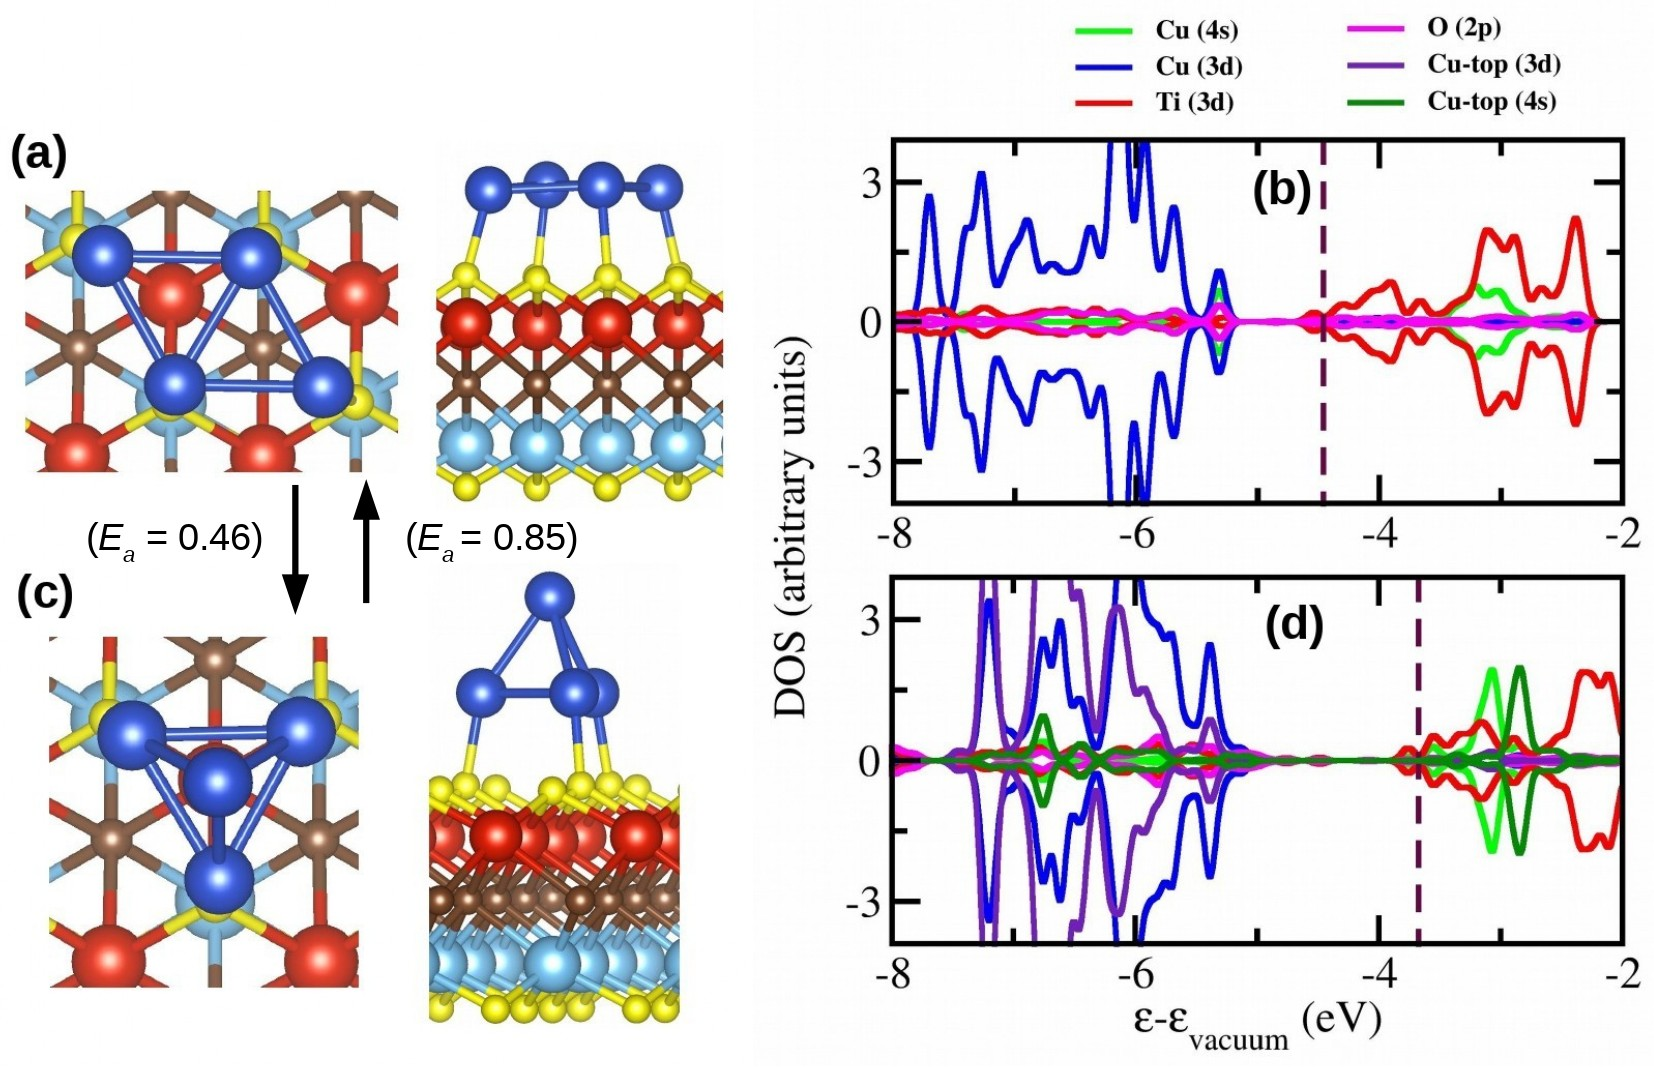
\includegraphics[width=12cm]{./Appendix3/figures/fig00.jpg} \\[0cm]
%    \end{array}$
% \end{center}
% \caption{Side view and top view of Cu$_4$ supported on Ti$_2$C (Cu$_4$/Ti$_2$CO$_2$) in (a) rhombus and (c) tetrahedral geometry. (c) and (d) shows the partial DOS projected on the Ti-$d$, Cu-$d$ and $s$ and O-$p$ states of rhombus-Cu$_4$/Ti$_2$CO$_2$ and tetrahedral-Cu$_4$/Ti$_2$CO$_2$ respectively\cite{mondal2020role}.}
%  \label{fig:00}
%\end{figure}


CO$_2$ is a very stable molecule with two unsaturated bonds which can be hydrogenated to produce many stable products like methanol, methane, carbon monoxide, formic acid and formaldehyde. As a result, the thermal reduction becomes a complex multi-step process where each of the elementary reaction needs a certain amount of activation energy to progress. In the case of Cu based thermal catalysts the intermediates and products are categorised into three notable pathways\cite{li2015heterogeneous, grabow2011mechanism, zhao2011insight, liu2015carbon, posada2016conversion} namely ``FORMATE", ``r-WGS (Reserve Water-Gas Shift) + CO hydrogenation" and ``trans-COOH". Our work explores the relationship between these pathways with the morphology of the ultra small copper cluster. Specifically, we have studied two catalysts, each containing a tetramer cluster of a particular shape, deposited on the 2D O-terminated Ti$_2$C MXene (Ti$_2$CO$_2$). The two shapes you have investigated are a tetrahedral shape and a rhombus shape, which are the most stable geometries on the surface and in the gas phase, respectively. The rhombus geometry is chosen because experimental techniques used to prepare the cluster catalysts include soft landing\cite{yin2014atomically,lu2014effect} which are agnostic of the cluster morphology and contains different shapes in the gas phase of which rhombus is the most populous. Moreover, the energy needed to convert the rhombus to the tetrahedra is around 0.46 eV which is higher than the initial step of CO$_2$ reduction discussed in the following section. Hence, the rhombus structure along with the tetrahedra have existence on the support. In the next subsection, we discuss the three pathways from the perspective of our tetramer catalysts.   

\subsection{Important reaction intermediates and pathways for CO\texorpdfstring{$_2$}{} reduction on Cu\texorpdfstring{$_4$}{}/Ti\texorpdfstring{$_2$}{}CO\texorpdfstring{$_2$}{} catalysts}

The complete reduction of CO$_2$ along each pathway is either methanol or methane. Zhong et al.\cite{zhong2020state} summarises the overall reduction profile over a Cu based thermal catalyst. However, in this present study, we restrict our investigation to the formation of methanol as the end product. The ``Formate" and ``r-WGS $+$ CO hydrogenation" produces formic acid and carbon monoxide as trademark products. In particular, ``trans-COOH" do not have a designated product and similar to the other pathways produce formaldehyde as by products. Although the intermediates and products are classified into these three pathways, it is quite possible for an intermediate in one pathway to transform into an intermediate of another pathway. Therefore, it is necessary to study all the competing reactions from a particular intermediate and then follow the one which is energetically most favourable. For each of the intermediates, various stable configurations were considered and the most stable one was considered. In the text, figures and tables, asterisk mark over any chemical formula suggests the intermediate (represented by the formula) is bound to the supported clusters. 

\begin{figure}
 \begin{center}
  $\begin{array}{c}
    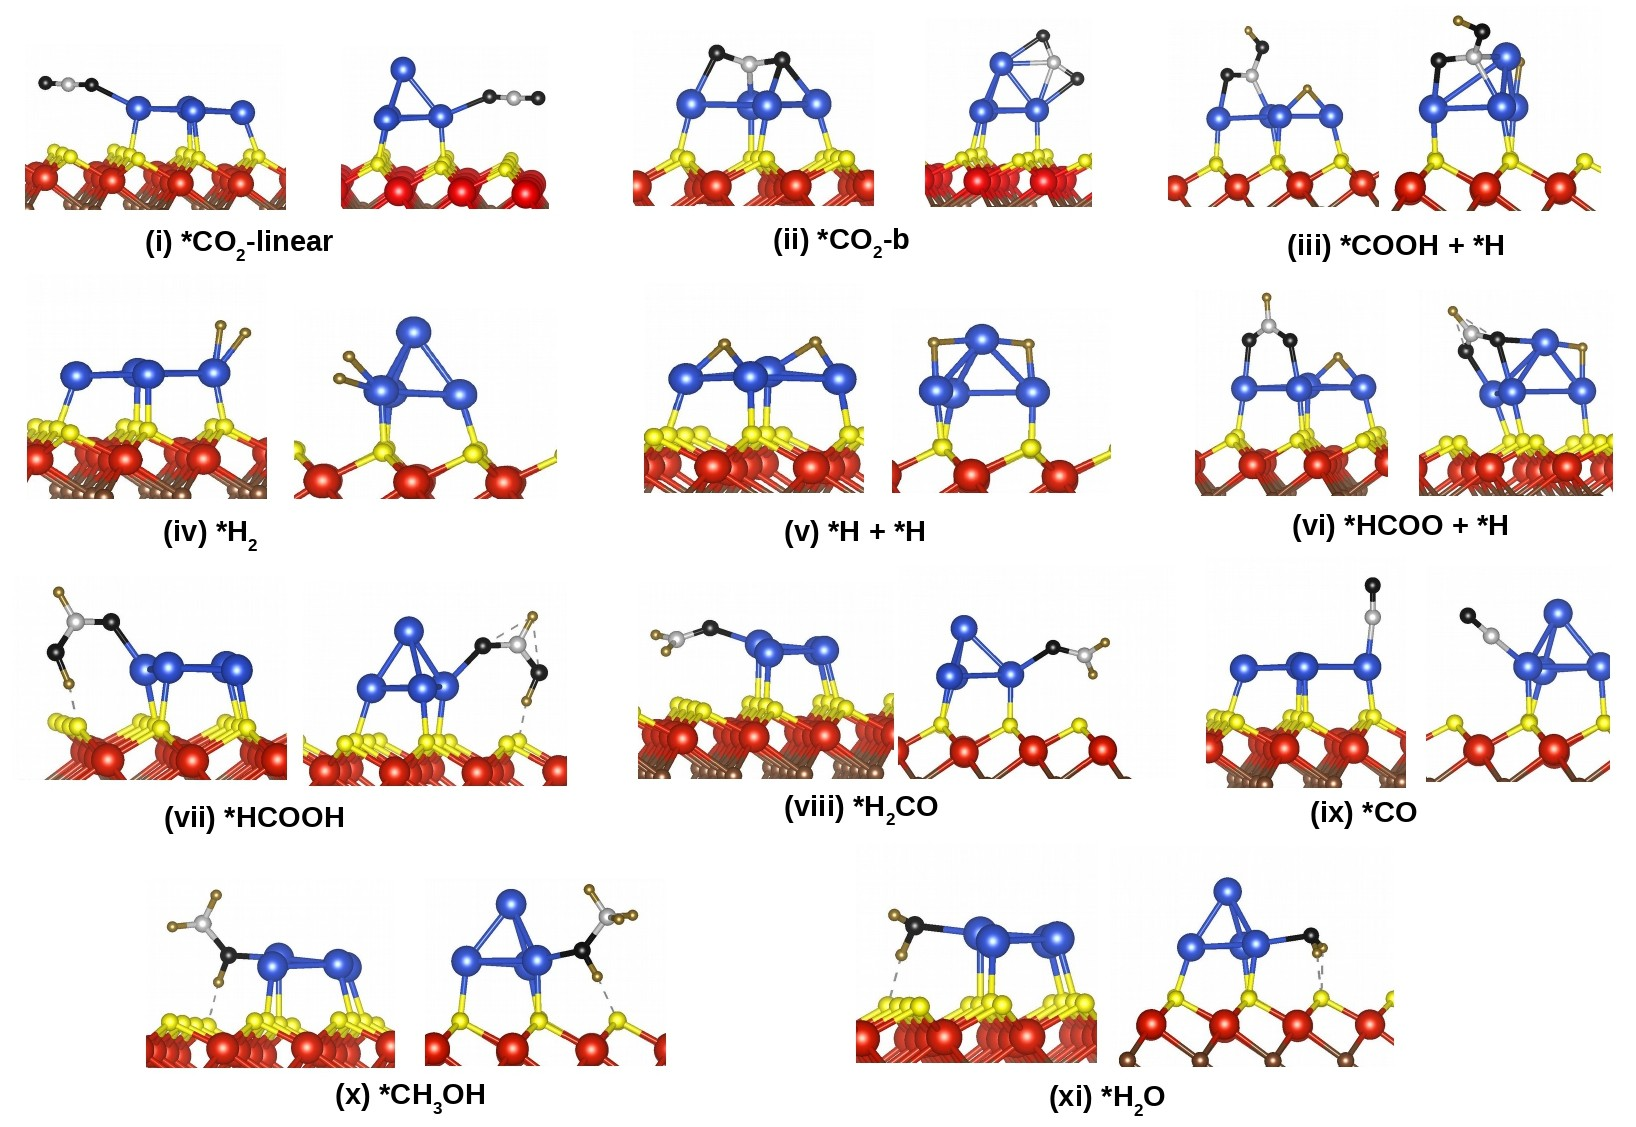
\includegraphics[width=14cm ]{./Appendix3/figures/fig01.jpg} \\[0cm]
    \end{array}$
 \end{center}
 \caption{Comparing the important intermediates and products on the rhombus (left) and tetrahedral (right) geometry of the supported tetramer cluster (Cu$_4$/Ti$_2$CO$_2$).}
  \label{fig:01}
\end{figure}

The reactants, CO$_2$ and H$_2$, do not interact with the Ti$_2$CO$_2$ support but adsorbs on the copper atoms of the tetramer clusters. Consequently, the MXene support does not provide any assistance in the CO$_2$ hydrogenation process. The most stable configuration of CO$_2$ adsorption on the supported clusters has been discussed in Section \ref{fooking} of Appendix \ref{appendix2}. On the other hand, H$_2$ binds to the positive Cu atom (Cu atom at the long diagonal of rhombus and basal Cu atom of the tetrahedron) of the tetramers (Figure \ref{fig:01} (iv)). In the adsorbed state, the H-H bond distance is elongated from 0.75 {\AA} in the gas phase to 0.82 (0.80) {\AA} on the rhombus (tetrahedron) tetramer. The binding energy of the H$_2$ molecule on the rhombus and tetrahedron tetramer are -0.27 eV and -0.30 eV respectively. However, at the typical reaction conditions of 500 K and near 1 bar pressure, the entropy effects make the desorption process of both the molecules more favourable (Table \ref{tab:2} column 3 and 5).

The first step of CO$_2$ hydrogenation follows either an Eley $-$ Rideal (ER) or a Langmuir $-$ Hinshelwood (LR) mechanism. In the former mechanism, either the CO$_2$ or H$_2$ adsorbs first and gets activated, which then interacts with the uninitiated molecular hydrogen / linear-CO$_2$. On the contrary, in the LH mechanism, CO$_2$ and H$_2$ coadsorbs on the cluster and then forms an intermediate where both the molecules are activated. Since both the molecules desorb at the operating temperature and pressure, it is less likely that the molecules will be simultaneously adsorbed. Moreover, activating both the molecules on the ultra small clusters will not be feasible due to the non-availability of adsorption sites. Therefore, the LH mechanism for CO$_2$ hydrogenation in the first step is not practical for ultra small tetramers. 

In the context of ER mechanism, the first elementary step is the adsorption and activation of either CO$_2$ or H$_2$. The adsorbed linear-CO$_2$ gets activated to the non-linear (bent) configuration (Figure \ref{fig:01} (ii)). The most stable bent form of the CO$_2$ on the rhombus (tetrahedron) has O-C-O bond angle of 118.2 (146.1)$^{\circ}$. The reaction is exothermic (-0.36 eV) on the rhombus whereas endothermic (0.40 eV) on the tetrahedron. The linear to bent form is an activated process and requires an activation energy of 0.14 eV and 0.42 eV on the rhombus and tetrahedron respectively. In the corresponding transition states (Figure \ref{fig:si-102} (1f) for rhombus and Figure \ref{fig:si-102} (2c) for tetrahedron) the O-C-O bond angles ($~$160$^{\circ}$) are between those observed in the gas phase and the bent intermediate. Additionally, the adsorbed CO$_2$ can be further activated through its auto dissociation into CO and atomic oxygen (O). The dissociation process is mildly exothermic on the rhombus (-0.04 eV) whereas mildly endothermic on the tetrahedron (0.14 eV). The activation needed to cross the TS is 0.47 eV on the rhombus (Figure \ref{fig:si-103} (1d)) and 1.36 eV on the tetrahedron (Figure \ref{fig:si-103} (2b) for tetrahedron). In the case of H$_2$, the activation is achieved by dissociating the molecule into atomic hydrogen atoms. In the most stable configuration on the rhombus, the dissociated hydrogen atoms are bound on the top at the opposite edges of the cluster whereas on the tetrahedron, the hydrogen atoms are at two adjacent edges shared by basal and atop Cu atoms (Figure \ref{fig:01} (v)). The dissociation process is exothermic (-1.19 eV for rhombus and -0.70 eV for tetrahedron) for either tetramers but the fluxional nature of rhombus\cite{mondal2020role} with respect to the tetrahedron drastically lowers the activation barrier from 0.96 eV on the tetrahedron to 0.25 eV on the rhombus. In the TS (Figure \ref{fig:si-101} (2b) for rhombus and Figure \ref{fig:si-101}  (3b) for tetrahedron) one of the hydrogen atoms slides into the hollow site formed by three copper atoms whereas the other stays on the original positive copper both ready to migrate into the stable edge sites. The H-H bond is elongated to 1.16 \AA{} on the rhombus whereas it is 1.92 \AA{} on the tetrahedron. 

In the next step, adsorbed H$_2$ (linear-CO$_2$) molecule reacts with the bent-CO$_2$ (dissociated atomic hydrogen) to generate the reduced intermediate along with an unreacted hydrogen atom. Depending on the atom of CO$_2$ that binds on to hydrogen we have two reduced products namely hydrocarboxyl (COOH) or formate (HCOO). HCOO formation is the first intermediate of the ``FORMATE" pathway whereas COOH sets the ``r-WGS + CO hydrogenation" and ``trans-COOH" pathways. Also, for the dissociated (*CO + *O), the hydrogen molecule attacks the CO to give (*COH + *O + *H) whereas an attack on O gives (*CO + *OH + *H). This path falls under the ``r-WGS + CO-hydrogenation" pathway. 

\noindent \textit{``FORMATE" pathway:} HCOO is the deciding intermediate for the ``FORMATE" pathway which binds bidentically through the oxygen atoms (Figure \ref{fig:01} (vi)). In the most stable configuration, the oxygen atoms of HCOO bind to the long and short diagonal of the rhombus whereas on the tetrahedron, one of the oxygen atoms bind to the basal Cu and the other bind at the adjacent edge shared by basal and atop copper atoms. HCOO is coadsorbed with an unreacted hydrogen atom, (*HCOO + *H) where both the species are more strongly (by 0.78 eV) bound to the rhombus compared to the tetrahedron. The adsorbed hydrogen atom further reduces HCOO to either formic acid (HCOOH, when attack is on the oxygen atom) or dioxymethylene (CH$_2$OO, when attack is on the carbon atom). In the most stable configuration (Figure \ref{fig:01} (vii)), HCOOH binds monodentically with the more positive Cu atom (long diagonal Cu atom of rhombus and basal Cu atom of tetrahedron) through the carbonyl oxygen such that the the hydroxyl hydrogen forms hydrogen bond (H-bond) with the support O$_{Ti_{2}CO_{2}}$. On the other hand, CH$_2$OO binds bidentically on either cluster. Since HCOOH is stable in the gas phase it desorbs from the rhombus and tetrahedron catalysts on obtaining an energy of -1.36 eV and -1.28 eV respectively. The structure and binding energy of all the gaseous intermediates adsorbed on the two catalysts are shown in Figure \ref{fig:01} and Table \ref{tab:2} respectively. 

On the rhombus, HCOOH is 0.57 eV less stable than CH$_2$OO whereas on the tetrahedron, HCOOH is 1.63 eV more stable than CH$_2$OO. The higher lability allows the bidentate interaction on the rhombus to be more favourable. In the next step, hydrogen from a new molecule of H$_2$, attacks HCOOH or CH$_2$OH to form CH$_2$OOH and an unreacted hydrogen atom. CH$_2$OOH much like CH$_2$OO bind bidentically through the oxygen atoms. Further, CH$_2$OOH auto-dissociates in the presence of the hydrogen atom to yield formaldehyde (CH$_2$O) and hydroxyl (OH). CH$_2$O (Figure \ref{fig:01} (viii)) is a stable molecule in the gas phase with a binding energy of -0.88 and -0.97 eV on the rhombus and tetrahedron respectively. Similar to HCOOH, CH$_2$O prefers to bind monodentically through the oxygen atom onto positive Cu for either tetramers and coadsorbed OH binds at the edge site. CH$_2$O gets further hydrogenated to methoxy (CH$_3$O) which binds mondentically through the oxygen atoms. A new molecule of H$_2$ further reduces the intermediates to CH$_3$OH and H$_2$O which forms the final product. It is to be noted that the formation of H$_2$O can occur at any stage after CH$_2$OOH dissociates. The exact chronology will depend on the activation energies of competing reactions. CH$_3$OH (Figure \ref{fig:01} (x)) and H$_2$O (Figure \ref{fig:01} (xi)) like other stable molecules prefers to bind monodentically to the the positive Cu atom through the hydroxyl oxygen such that the OH group forms H-bond with the support O$_{Ti_{2}CO_{2}}$. The binding energy of CH$_3$OH (H$_2$O) on rhombus and tetrahedra are -1.15 eV (-0.88 eV) and -1.21 eV (-1.01 eV). 

\noindent \textit{``r-WGS + CO-hydrogenation" and ``trans-COOH" pathways:} COOH forms the decisive intermediate for both the ``r-WGS + CO-hydrogenation" and ``trans-COOH" pathways. In the most stable configuration (Figure \ref{fig:01} (iii)), COOH binds bidentically with the carbon and oxygen atom. On the rhombus, the carbon (oxygen) binds to the short (long) diagonal copper atom whereas, on the tetrahedron, the carbon binds at the edge shared by the atop and basal copper and the oxygen binds to the adjacent basal copper atom. (*COOH + *H) is 0.21 eV more stable on the rhombus compared to the tetrahedron. Trans-COOH is a conformer of COOH where the OH bond is directed away from the carbonyl group. 

COOH is coadsorbed with hydrogen (*COOH + *H) and can react to form dihydroxycarbene, C(OH)(OH), which starts the ``trans-COOH" pathway. The carbon atom of COHOH monodentically binds to the positive Cu atom. The binding energy of C(OH)(OH) on either cluster is very weak (-0.1 eV). C(OH)(OH) self dissociates to form hydroxymethylidyne (*COH + *OH). The carbon atom of COH monodentically binds to Cu atoms at the face of either cluster. On further hydrogenation COH reduces to hydroxymethylene (HCOH) followed by hydroxymethyl (H$_2$COH). In the most stable configuration, HCOH binds monodentically to the positive Cu through its carbon atom whereas CH$_2$OH binds bidentically through the carbon and hydroxyl oxygen atoms at the cluster edges. (*HCOH + *OH + *H) and (*CH$_2$OH + *OH) is found to be respectively 0.24 eV and 0.50 eV more stable on the rhombus than the tetrahedron. In the final hydrogenation step, CH$_2$OH reduces to CH$_3$OH and the OH to H$_2$O. Similar to the formate pathway, H$_2$O formation can occur at any stage post dissociation of COHOH to COH and OH. 

If COOH auto dissociates before reacting with hydrogen atom, the product is (*CO + *OH + *H). The direct C-O bond dissociation of activated CO$_2$ can also result in CO formation along with coadsorbed oxygen atom. The coadsorbed oxygen atom prefers to bind at the face of the cluster interacting with three Cu atoms. In either scenario, we get CO (Figure \ref{fig:01} (ix)) as an intermediate which completes the ``r-WGS" pathway and marks the beginning of ``CO hydrogenation" pathway. In the most stable configuration of both the tetramers, CO likes to bind to the positive Cu atom through the carbon atom. The binding energies of CO on the rhombus and the tetrahedron are -1.28 eV and -1.19 eV. In the case of direct CO formation, (*CO + *O), oxygen can be hydrogenated to form (*CO + *OH + *H). The unreacted hydrogen atom attacks the carbon atom of CO to form formyl (HCO) or the oxygen atom to form COH. Formation of COH enters the ``trans-COOH" pathway. In the most stable configuration, HCO likes to bind bidentically and the intermediate (*HCO + *OH + *H) is comparatively more stable on the rhombus by 0.49 eV. HCO reacts with a new molecule of H$_2$ to either become HCOH and generate the intermediates formed in the ``trans-COOH" pathway or form H$_2$CO and follow the ``FORMATE" pathway.

\begin{table}

 \caption{Binding energy of molecules on the rhombus (Rh) and tetrahedral (Th) tetramers (Cu$_4$/Ti$_2$CO$_2$) without ($E_{bind}$) and with ($E^S_{bind}$) entropy corrections (at 500 K and 1 bar pressure.)}
 \label{tab:2}
  \begin{center}
\resizebox{\textwidth}{!}{  
  
    \begin{tabular}{|* {5}{c|}}
  
    \hline
   Reaction & \multicolumn{1}{c|}{$E_{bind}$ (Rh)} &\multicolumn{1}{c|}{$E^S_{bind}$ (Rh)}& \multicolumn{1}{c|}{$E_{bind}$ (Th)} &\multicolumn{1}{c|}{$E^S_{bind}$ (Th)}\\ \hline
  
 * + H$_2$(g)   $\rightarrow$ *H$_2$          &-0.27    &0.48   &-0.30   &0.45  \\ \hline
 * + CO$_2$(g)  $\rightarrow$ *CO$_2$         &-0.37    &0.85   &-0.41   &0.81   \\ \hline
 * + HCOOH(g)   $\rightarrow$ *HCOOH          &-1.36    &0.07   &-1.28   &0.15  \\ \hline
 * + CH$_2$O(g) $\rightarrow$ *CH$_2$O        &-0.88    &0.35   &-0.93   &0.31  \\ \hline
 * + CO(g)      $\rightarrow$ *CO             &-1.28    &-0.18  &-1.19   &-0.09  \\ \hline
 * + H$_2$O(g)  $\rightarrow$ *H$_2$O         &-0.88    &0.19   &-1.01   &0.05  \\ \hline
 * + CH$_3$OH(g) $\rightarrow$ *CH$_3$OH      &-1.15    &0.23   &-1.21   &0.17  \\ \hline

  \end{tabular}
 }
  \end{center}
\end{table} 

In this next section, we reported the main intermediates of the three pathways observed over the supported Cu tetramers. In the following two sections we present the complete reaction profile of CO$_2$ hydrogenation over the rhombus and tetrahedral catalysts respectively. During the characterization of the reaction profile we discontinued the competing reactions having higher activation barriers. It is to be noted that the relatively unfavourable reactions are likely to occur at some point but will have a lower probability.   
 
\subsection{CO\texorpdfstring{$_2$}{} reduction on the rhombus geometry of Cu\texorpdfstring{$_4$}{}/Ti\texorpdfstring{$_2$}{}CO\texorpdfstring{$_2$}{}}

According to the ER mechanism in the ultra small clusters, we investigate the activation of CO$_2$ (linear to bent) and H$_2$ (H$_2$ to atomic hydrogen atoms) separately. We find both the reactions are exothermic and require an activation energy of 0.14 eV (H$_2$ activation) and 0.25 eV (CO$_2$ activation). Although the energy barriers are small and comparable, in order to limit the numerous possibilities, we limit our investigation to the competing process with the lowest barrier. We also neglect the competing back reaction for any exothermic reaction and only consider for reactions that are endothermic. In the forthcoming discussion we have applied the same logic and reported our results accordingly. Therefore, CO$_2$ activation  (Figure \ref{fig:02} (i) and (ii)) becomes the first step in the reduction process on the rhombus tetramer.  

In the absence of coadsorbed H$_2$, bent-CO$_2$ auto dissociates into (*CO + *O). This auto dissociation of CO$_2$ is a mild exothermic process of -0.04 eV and needs an activation energy of 0.45 eV (Figure \ref{fig:si-103} (1d)). The binding energy of CO in the presence of coadsorbed oxygen is -1.30 eV (-0.20 after entropy corrections). In the event that CO does not desorb, two possibilities arise. First, the adsorbed oxygen atom on the availability of H$_2$ molecule reduces to (*OH + *H) and then finally to H$_2$O (Figure \ref{fig:si-105} (1b)). The reduction of *O to *OH in the presence of CO is a highly exothermic process -1.05 eV and needs an activation energy of 0.53 eV (Figure \ref{fig:si-104} (1b)). Second, hydrogenation of CO to HCO (COH) in the presence of atomic oxygen is possible. However, these two reactions are endothermic (1.17 eV for HCO and 1.97 eV for CHO)  and requires more energy than either CO desorption or *O reduction to OH. The former process of hydrogenating CO$_2$ to CO and H$_2$O is the ``r-WGS" reaction. 

If the bent-CO$_2$ is in the vicinity of coadsorbed H$_2$ molecule, the hydrogen atom of H$_2$ dissociatively attacks either the carbon atom of CO$_2$ to form COOH (Figure \ref{fig:02} (iv.a)) or the oxygen atom to form HCOO. Both the processes are endothermic (-0.51 eV for COOH and -1.89 eV for HCOO) but the formation of COOH has a lower activation barrier (0.45 eV) (Figure \ref{fig:si-106} (1b)) with respect to HCOO (0.86) (Figure \ref{fig:si-107} (1b)). As a result, (*COOH + *H) is more likely to form than (*HCOO + *H). COOH in the presence of atomic hydrogen undergoes three competing reactions. First, COOH auto dissociates into CO and OH in the presence of hydrogen atom. Second, atomic hydrogen attacks the carbon atom of COOH to form HCOOH. Third, atomic hydrogen attacks carbonyl oxygen of COOH to form C(OH)(OH). The first reaction is exothermic (-0.47 eV) and requires an activation energy of 0.29 eV (Figure \ref{fig:si-109} (1b)). The second and third paths are endothermic (0.33 and 1.77 eV respectively). The formation of HCOOH goes through a meta stable intermediate which is 0.82 eV higher than the initial state (*COOH + *H). Therefore, both the second and third reactions would require a minimum activation of 0.82 and  1.77 eV respectively which is higher than the activation needed for dissociating COOH into CO and OH. As a result, COOH dissociation is the most likely process to occur. 
Irrespective of the immediate presence or absence of coadsorbed H$_2$ with bent CO$_2$, we find the formation of (*CO + *OH + *H) to be inevitable. Since HCOO, HCOOH and C(OH)(OH) are less likely to form, we expect the reduction process to not follow the ``FORMATE" and ``trans-COOH" pathway. In the following step, we have four competing reactions. First (Second), formation of HCO (COH), when the atomic hydrogen attacks the carbon (oxygen) atom of CO in the presence of OH. Third, when hydrogen attacks OH to form H$_2$O in the presence of CO. Fourth, desorption of CO, when supplied with an energy of -1.28 eV (-0.18 eV after entropy corrections). The formation of CHO (Figure \ref{fig:02} (vi)) and COH belongs to the ``CO-hydrogenation" and ``trans-COOH" pathway whereas formation of H$_2$O along with CO belong to ``r-WGS" pathway. The formation of (*HCO + *OH), (*COH + *OH) and (*CO + *H$_2$O) are all endothermic (0.58 eV, 1.49 eV and 0.81 eV respectively) which considerably enhances the possibility of backward reaction. The activation energy needed for HCO, COH and H$_2$O formation is 1.32 eV (Figure \ref{fig:si-109} (2b)), (a minimum of) 1.49 eV and 1.33 eV (Figure \ref{fig:si-112} (1b)) respectively. Among the four competing reactions, CO desorption requires the least amount of energy and will be the most likely process. After the desorption of CO, the remaining (*H + *OH) species recombine on gaining 1.21 eV of energy (Figure \ref{fig:si-105} (1b)). H$_2$O formed under entropy effects desorbs without any activation. The overall process becomes part of the ``r-WGS" pathway. Moreover, an attack of hydrogen atom on OH in the presence of non-participating CO to produce (CO + H$_2$O) needs more energy than CO desorption. As a result, (CO + H$_2$O) formation enters into the above mentioned step wise CO desorption and (*H + *OH) recombination. Experimentally\cite{zhong2020state,riaz2013review}, membrane based reactor selectively removes H$_2$O and recycles CO with unreacted reactants (*CO$_2$ + *H$_2$). The process becomes the part of syn gas reduction which is out of the scope of the present work. 

If the hydrogen attacks the CO before its desorption in the presence of OH, formation of (*HCO + *OH) will be the most likely process. Further, in the absence of any coadsorbed H$_2$, backward process of HCO dissociation to (*CO + *H) is possible and will require an activation energy of 0.88 eV. However, in the presence of coadsorbed H$_2$, hydrogenation of HCO or OH will compete with the backward dissociation of HCO to (*CO + *H). Depending on the site of attack by the atomic hydrogen three competing reactions are possible. First, hydrogen attacks OH to form H$_2$O. Second (Third), atomic hydrogen attacks carbon (oxygen) of HCO to form CH$_2$O (HCOH). All the three processes are exothermic (-0.21 eV, -0.14 eV and -0.08 eV respectively) and require an activation energy of 0.62 eV (Figure \ref{fig:si-112} (2b)), 0.76 eV (Figure \ref{fig:si-112} (3b)) and 0.17 eV (Figure \ref{fig:si-110} (1b)) respectively. Therefore, the formation of HCOH (Figure \ref{fig:02} (viii)) over the other two processes is more likely. Moreover, the lower activation barrier for HCOH than the backward dissociation of HCO to CO will ensure the continuity of the reduction process. In the next step, hydrogen from the coadsorbed species, (*HCOH + *OH + *H), attacks the carbon of HCOH to form CH$_2$OH (Figure \ref{fig:02} (ix)). The process is highly exothermic (-0.63 eV) and requires an activation of 0.70 eV (Figure \ref{fig:si-110} (2b)). If the atomic hydrogen attacks the OH, H$_2$O is formed in the presence of HCOH. This process is mildly endothermic (0.15 eV) and requires an activation of 1.19 eV. The lower energy requirement for CH$_2$OH formation makes it more likely to form.  

In the penultimate step, another coadsorbed H$_2$ molecule attacks either CH$_2$OH or OH. If the attack is on CH$_2$OH, methanol (CH$_3$OH) along with (*OH + *H) are formed whereas if OH is attacked (*H$_2$O + *CH$_2$OH + *H) is formed (Figure \ref{fig:02} (xi)). The formation of CH$_3$OH is an exothermic process (-0.95 eV) but requires an activation of 1.72 eV (Figure \ref{fig:si-111} (2b)). On the other hand, formation of H$_2$O in the presence of CH$_2$OH is mildly endothermic (0.14 eV) and require an activation of mere 0.33 eV (Figure \ref{fig:si-110} (3b)). Clearly, formation of water in the presence of H and CH$_2$OH is energetically more favourable. As the reaction is endothermic, backward process of H$_2$O dissociation with activation energy of 0.19 eV is possible but entropy effects ensure the desorption to be the most favourable option. At the very end, the coadsorbed hydrogen and CH$_2$OH (Figure \ref{fig:02} (xii) combine to produce CH$_3$OH (Figure \ref{fig:02} (xiii) and the process is again mildly endothermic (0.19 eV) with an activation barrier of 1.35 eV (Figure \ref{fig:si-111} (2b)). Much like water, methanol desorbs without the need of any activation and probability of back reaction remains very less. 
 
\begin{figure}
 \begin{center}
  $\begin{array}{c}
    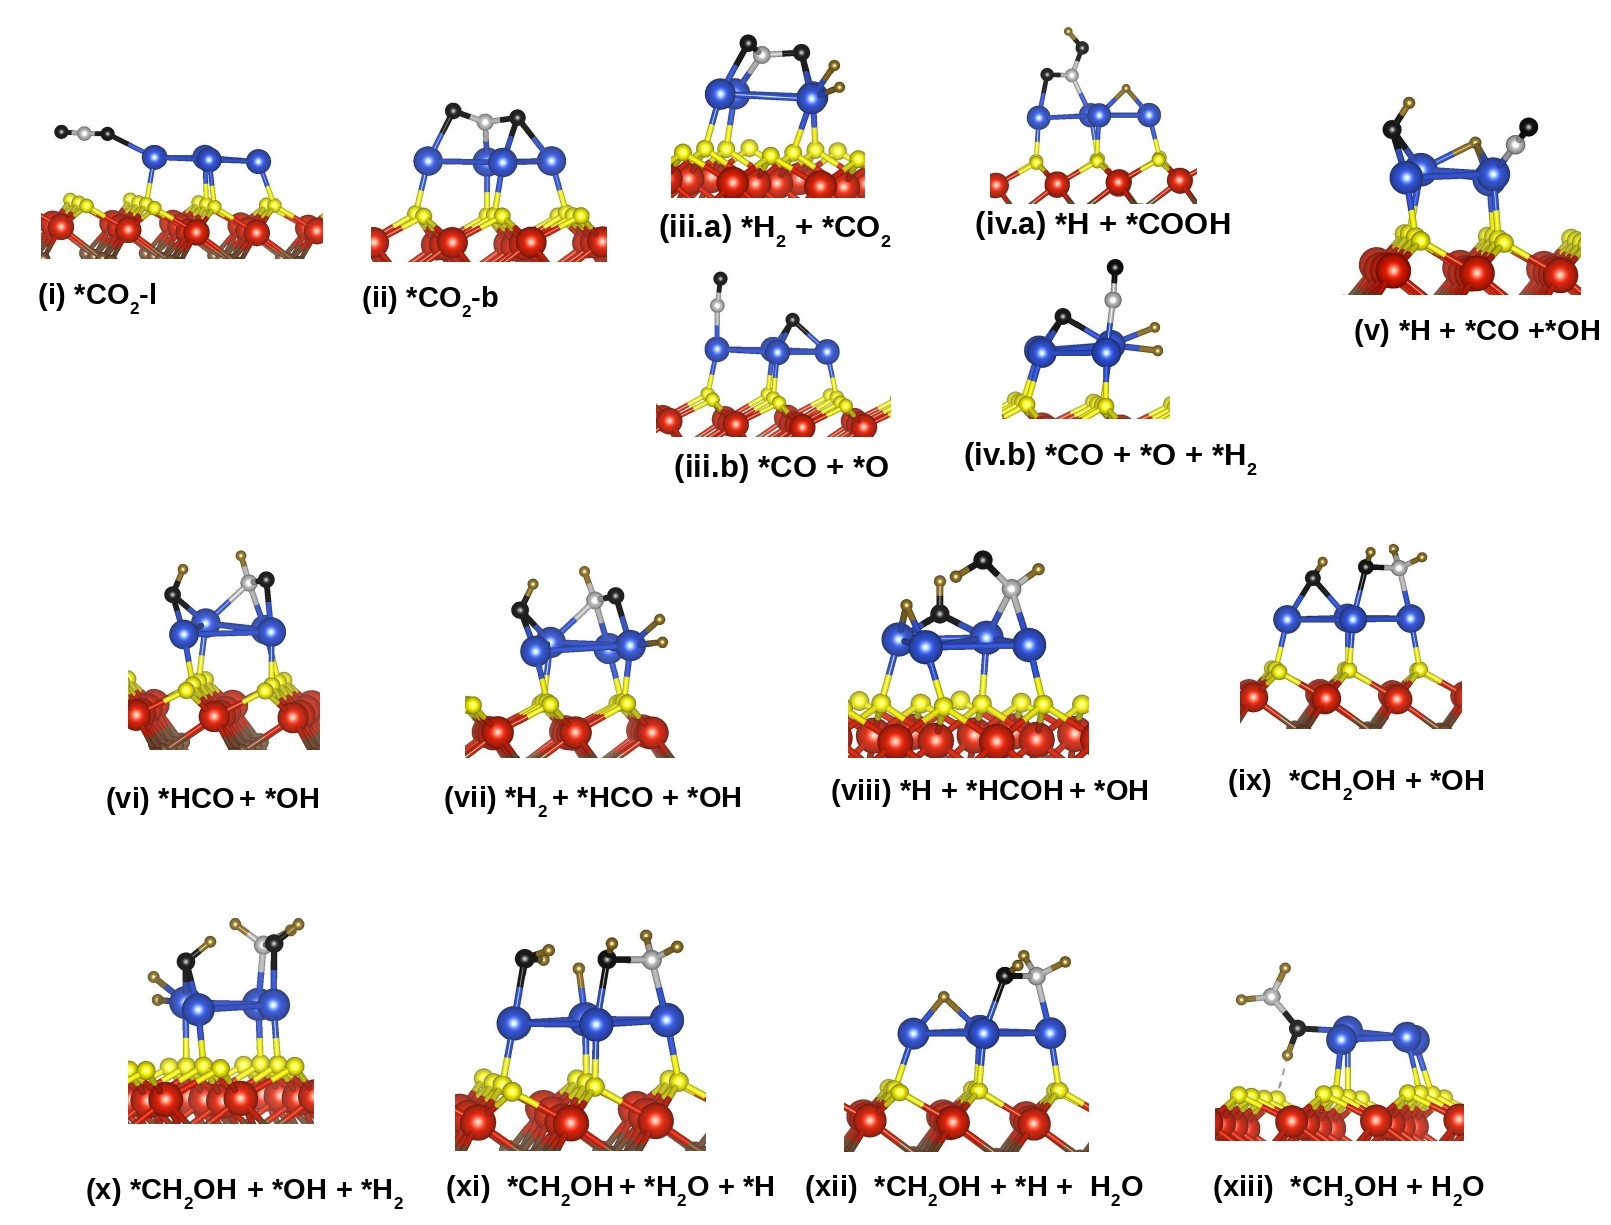
\includegraphics[width=14cm ]{./Appendix3/figures/fig02.jpg} \\[0cm]
    \end{array}$
 \end{center}
 \caption{The intermediates and products of CO$_2$ reduction formed on the rhombus-Cu$_4$/Ti$_2$CO$_2$ along the most probable (primary) route. The intermediates formed are numbered in ascending order. }
  \label{fig:02}
\end{figure}

The energetic of the complete process with respect to the E$_{ref}$ is reported in Table \ref{tab:1} (column 1 contains the name of intermediate species and column 2 shows E$_{ref}$) and Figure \ref{fig:05a}. The flowchart for the overall process is shown in Figure \ref{fig:04} (a). CO$_2$ hydrogenation (reduction) on the rhombus tetramer is an activated process and produces CO as the major product. The formation of CO requires an effective activation of 0.40 eV which corresponds to CO$_2$-bent $\rightarrow$ (*CO + *O). However, the formation of H$_2$O from adsorbed (*OH + *H) is the rate determining step (RDS) with an activation energy of 1.21 eV. Additionally, CO is also generated when COOH auto dissociates along the C-O bond (*COOH + *H $\rightarrow$ *CO + *OH + *H). The formation of methanol is possible if and only if the CO does not desorb. The overall process needs an effective activation of 1.35 eV corresponding to the reduction of CH$_2$OH to CH$_3$OH (RDS: CH$_2$OH + H $\rightarrow$ CH$_3$OH). The relatively higher energy demands for the formation of HCOO compared to COOH renders the ``FORMATE" process less probable. Also, the ``trans-COOH" intermediate is less stable compared to the (CO + OH + H) intermediate. From the above discussion, we conclude that the ``r-WGS" pathway is predominant (primary) on the rhombus and is achieved either through the direct dissociation of CO$_2$ or the dissociation of COOH. However, with an increase of CO partial pressure one might expect the ``CO-hydrogenation" pathway to generate methanol and other products via the (CO + OH + H) intermediate. 


%\begin{figure}
% \begin{center}
%  $\begin{array}{c}
%    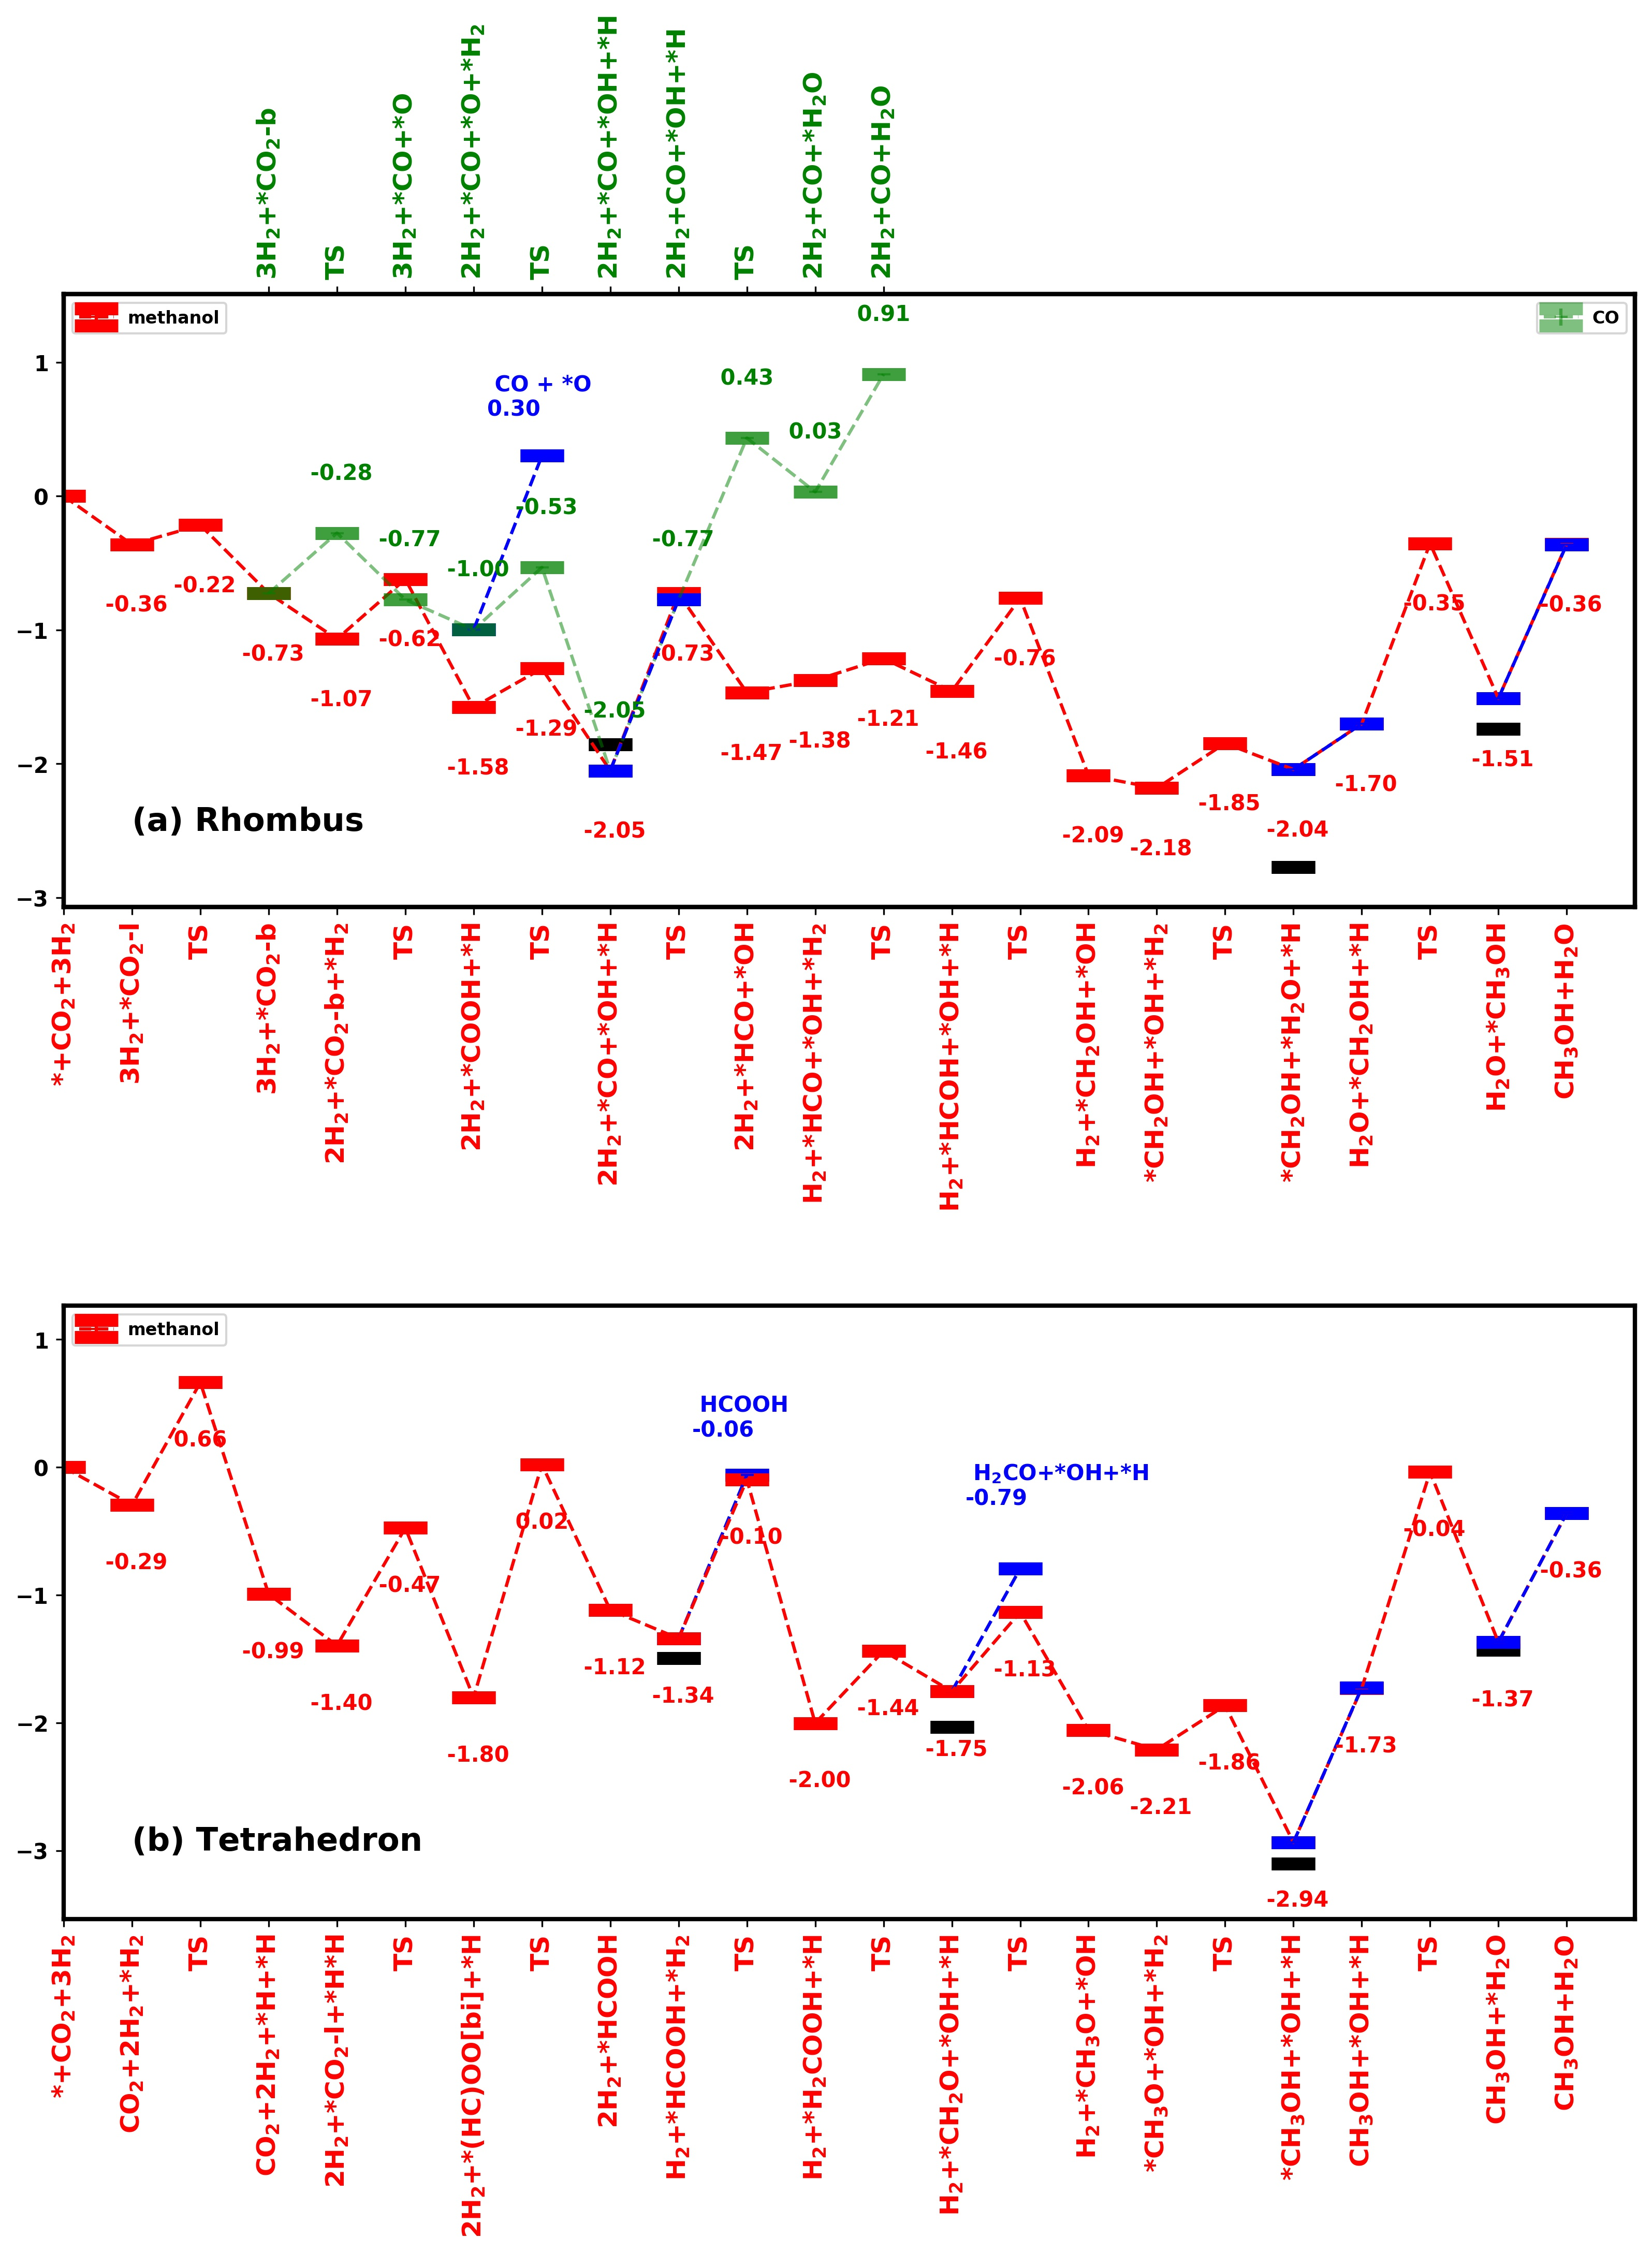
\includegraphics[width=12cm ]{./Appendix3/figures/fig05.jpg} \\[0cm]
%    \end{array}$
% \end{center}
% \caption{The most probable (primary) reaction profile for rhombus (top panel) and tetrahedral (bottom panel) tetramer supported on Ti$_2$CO$_2$. Blue level and graph shows the desorption of different gaseous molecules. Black levels represent the desorption energy of molecules with entropy corrections. }
%  \label{fig:05}
%\end{figure}

\begin{figure}
 \begin{center}
  $\begin{array}{c}
    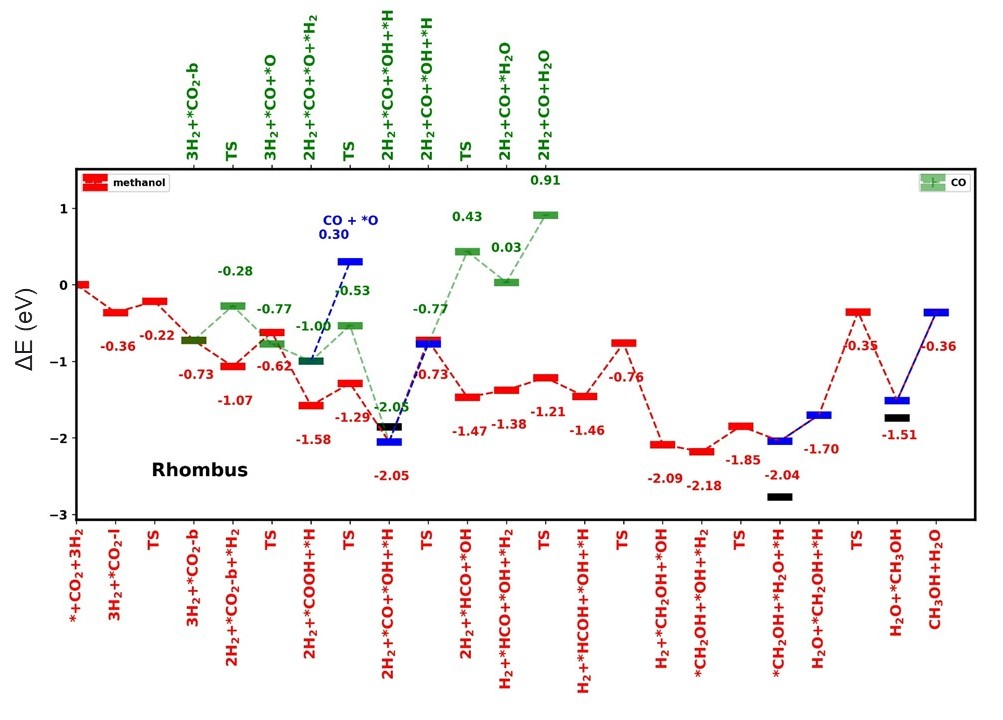
\includegraphics[width=14cm ]{./Appendix3/figures/fig05a.jpg} \\[0cm]
    \end{array}$
 \end{center}
 \caption{The most probable (primary) reaction profile for CO$_2$ reduction on rhombus-Cu$_4$/Ti$_2$CO$_2$. Blue levels show the desorption of stable molecules. Black levels correspond to the desorption energy of the stable molecules with entropy corrections. $\Delta E$ is the change in energy of the intermediates with respect to the $E_{ref}$.}
  \label{fig:05a}
\end{figure}

\subsection{CO\texorpdfstring{$_2$}{} reduction on the tetrahedral geometry of Cu\texorpdfstring{$_4$}{}/Ti\texorpdfstring{$_2$}{}CO\texorpdfstring{$_2$}{}}

\begin{figure}
 \begin{center}
  $\begin{array}{c}
    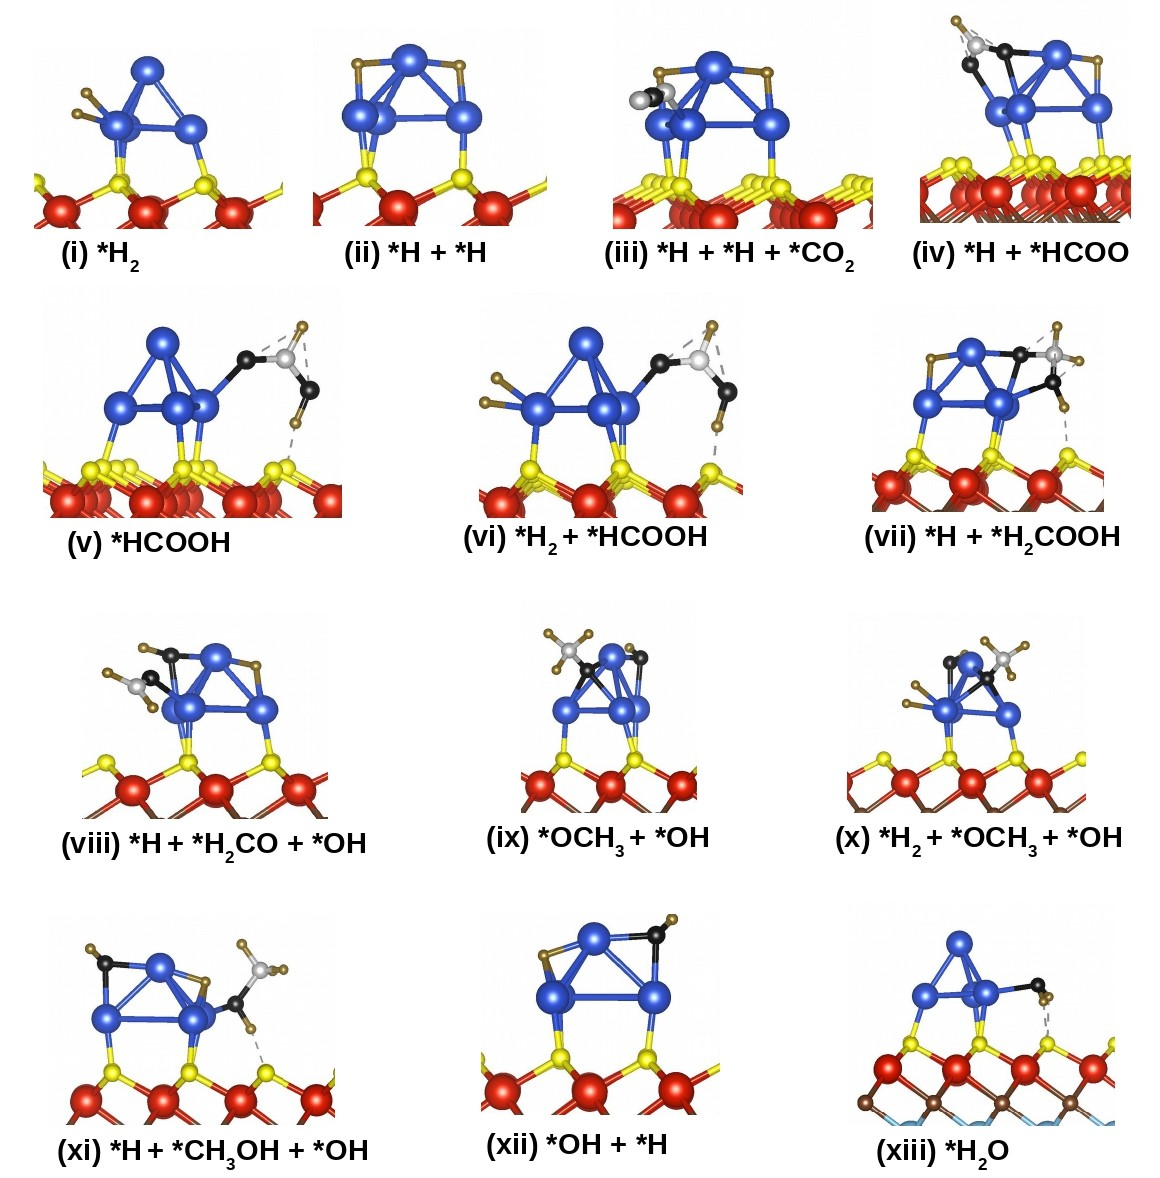
\includegraphics[width=14cm ]{./Appendix3/figures/fig03.jpg} \\[0cm]
    \end{array}$
 \end{center}
 \caption{The intermediates and products of CO$_2$ reduction formed on the tetrahedron-Cu$_4$/Ti$_2$CO$_2$ along the most probable (primary) route. The intermediates formed are numbered in ascending order.}
  \label{fig:03}
\end{figure}

\begin{figure}
 \begin{center}
  $\begin{array}{c}
    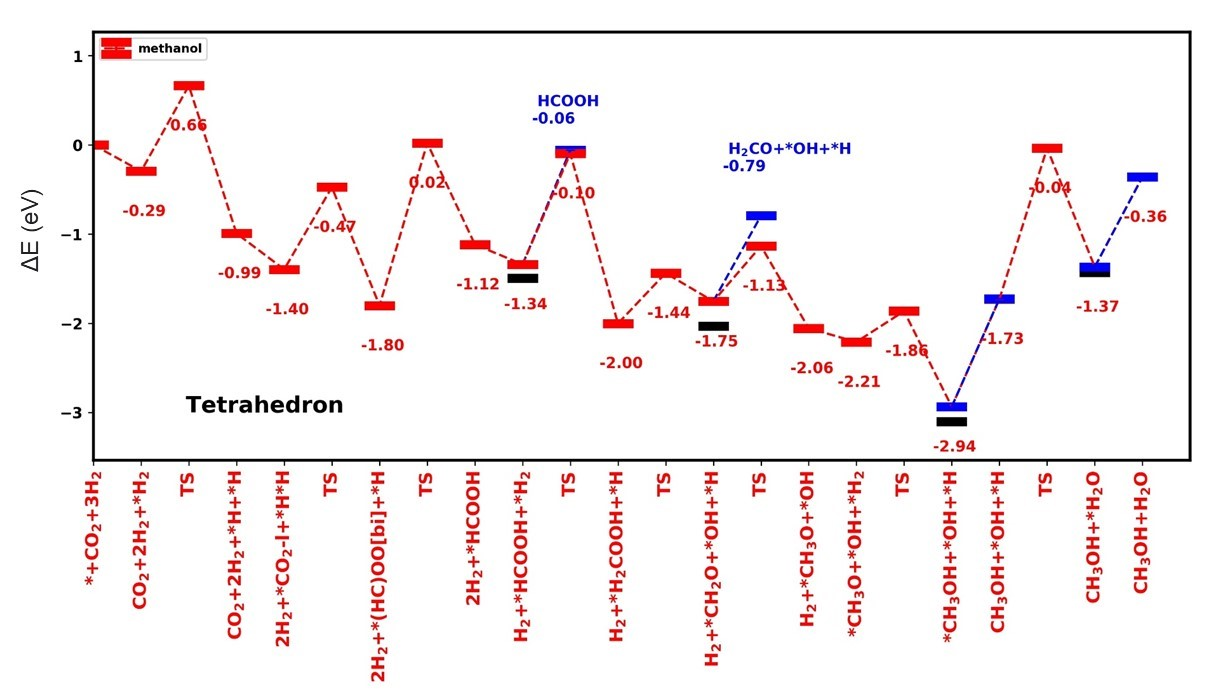
\includegraphics[width=14cm ]{./Appendix3/figures/fig05b.jpg} \\[0cm]
    \end{array}$
 \end{center}
 \caption{The most probable (primary) reaction profile for CO$_2$ reduction on tetrahedron-Cu$_4$/Ti$_2$CO$_2$. Blue levels show the desorption of stable molecules. Black levels correspond to the desorption energy of the stable molecules with entropy corrections. $\Delta E$ is the change in energy of the intermediates with respect to the $E_{ref}$..}
  \label{fig:05b}
\end{figure}

Similar to the case in rhombus, the binding strengths of CO$_2$ (-0.41 eV) and H$_2$ (-0.30 eV) are comparable on the tetrahedral tetramer. However, the entropy effects desorb them without any activation. The increase of partial pressure of the gases enhance the respective binding strengths. The tetrahedral geometry of the tetramer is the most stable configuration on the MXene. In view of the ER mechanism, the activation of CO$_2$ from linear to bent is endothermic (0.40 eV) and has an activation barrier of 0.42 eV  (Figure \ref{fig:si-102} (2c)) which suggests the backward process needs no energy. Additionally, auto dissociation of CO$_2$ to CO and O is mildly endothermic (0.14 eV) and requires an activation of 1.36 eV (Figure \ref{fig:si-103} (2b)). However, activation of H$_2$ to dissociated H atoms (Figure \ref{fig:03} (i) and (ii)) is highly exothermic (-0.70 eV) with an activation barrier of 0.96 eV (Figure \ref{fig:si-101} (3b)). On comparing the activation of CO$_2$ and H$_2$ on the tetrahedral cluster we find the dissociation of H$_2$ into atomic hydrogen atoms is the first step to start the reduction process. One of the dissociated hydrogen atoms attacks the coadsorbed CO$_2$ to form either COOH or HCOO. The formation of COOH is endothermic (0.13 eV) with an activation barrier of 2.05 eV (Figure \ref{fig:si-117} (1c)) whereas the formation of HCOO is exothermic (-0.40 eV) with a comparatively smaller activation barrier of 0.92 eV (Figure \ref{fig:si-113} (1c)).

The formation of HCOO  (Figure \ref{fig:03} (iv)) over COOH, indicates the preference of tetrahedral tetramer towards the ``FORMATE" pathway. The reduction via the ``r-WGS" and ``trans-COOH" pathway is less probable. The remaining hydrogen atom attacks the carbon (oxygen) of HCOO to form H$_2$COO (HCOOH). H$_2$COO formation is highly endothermic (1.57 eV) and needs an activation of 2.33 eV (Figure \ref{fig:si-115} (2f)). On the other hand, HCOOH (Figure \ref{fig:03} (v)) formation is comparatively less endothermic (0.68 eV) and needs 1.82 eV (Figure \ref{fig:si-108} (2b)) to overcome the energy barrier. Therefore, formation of HCOOH is more likely than H$_2$COO but the endothermic nature of the reaction introduces the possibility of backward reaction which only requires 1.27 eV. 

In the next step, we have three competing reactions. First, back reaction of HCOOH to (*HCOO + *H). Second, desorption of HCOOH which at said reaction conditions does not require any activation. Third, in the presence of coadsorbed H$_2$, hydrogen attacks the carbon atom of HCOOH to form CH$_2$OOH (Figure \ref{fig:03} (vii)). The third process is exothermic (-0.66 eV) and needs an activation of 1.24 eV (Figure \ref{fig:si-113} (2b)). Among the above possibilities, desorption of HCOOH is energetically the most favourable. However, in the case HCOOH does not desorb, further hydrogenation or dissociation of HCOOH becomes a possibility. In the absence of a new molecule of H$_2$, the backward dissociation of HCOOH to (*HCOO + *H) is most likely. However, in the presence of coadsorbed H$_2$ molecule, HCOOH gets hydrogenated to CH$_2$OOH and would require a minimum of 1.24 eV. Further, the CH$_2$OOH intermediate auto dissociates into CH$_2$O and OH (Figure \ref{fig:03} (viii)). This process is endothermic (-0.25 eV) and requires an activation of 0.56 eV (Figure \ref{fig:si-114} (1b)). 

After the formation of (*CH$_2$O + *OH + *H), we face with five competing reactions. First, back reaction with a small activation of 0.32 eV due to the endothermic nature of CH$_2$O formation. Second, desorption of CH$_2$O with no activation. Third, attack of coadsorbed hydrogen on OH to form H$_2$O. Fourth (Fifth), attack of hydrogen on carbon (oxygen) of CH$_2$O to form CH$_3$O (CH$_2$OH). The third process is endothermic (0.28 eV) and would need 1.83 eV to cross the energy barrier. However, fourth and fifth are exothermic (-0.30 eV and -0.03 eV). The activation barrier for the fourth path (CH$_3$O formation) is 0.62 eV (Figure \ref{fig:si-114} (2d)). As CH$_2$O binds to the Cu atom through the oxygen atom, the attack of hydrogen on the oxygen atom of CH$_2$O to form CH$_2$OH is sterically hindered. Hence, the overall process first requires the molecule to desorb and then the attack of hydrogen is facilitated. As CH$_2$O gets desorbed, the possibility of CH$_2$OH formation becomes less probable. Out of the five, desorption of H$_2$CO is the most favourable. If the OH or H attacks the H$_2$CO before its desorption, the backward process of CH$_2$OOH formation or CH$_3$O formation becomes feasible. The lower energy requirement of the backward process makes it second most probable. However, the formation of CH$_3$O with an activation of 0.62 eV is also a possibility. If (*CH$_3$O + *OH) is formed, we find two competing reactions. First (Second), in the presence of H$_2$ molecule, hydrogenation of OH (CH$_3$O) to form H$_2$O (CH$_3$OH). The unavailability of H$_2$ coadsorption site near the OH reduces our search to CH$_3$OH formation which is an exothermic process (0.73 eV) and needs an activation of 0.34 eV. The last elementary reaction is the recombination of *H and *OH to form H$_2$O (Figure \ref{fig:03} (xii) and (xiii)) followed by its desorption. The recombination is endothermic (0.36 eV) and requires an activation of 1.69 eV (Figure \ref{fig:si-105} (2b)). 




The energetic of the complete process with respect to the E$_{ref}$ are reported in Table \ref{tab:1} (column 3 for intermediate species and 4 for the E$_{ref}$) and Figure \ref{fig:05b}. The flowchart for the overall process is shown in Figure \ref{fig:04} (b). Similar to the rhombus tetramer, CO$_2$ reduction on the tetrahedral geometry is also an activated process. The main product of the reaction is HCOOH which needs an effective activation of 1.82 eV corresponding to the hydrogenation of HCOO to HCOOH (RDS: *HCOO + *H $\rightarrow$ *HCOOH). Provided that the HCOOH does not desorb, further reduction generates CH$_2$O at first and finally reduces to CH$_3$OH. Both the products share the same RDS as HCOOH. Since the formation of COOH needs more energy compared to HCOO, the ``r-WGS" and ``trans-COOH" pathways are less accessible. As a result, the higher probability of HCOO formation drives the overall reduction reaction to the ``FORMATE" pathway on the tetrahedral cluster. 


\begin{table}[htbp!]

 \caption{Relative energies of the intermediates for the supported rhombus and tetrahedron tetramers. $\Delta E = E_{A+B}^{ZPE} - E_{ref}$ where $\Delta E$ is the relative energy of the intermediate with respect to the reference energy ($E_{ref}$).  }
 \label{tab:1}
  \begin{center}
\resizebox{\textwidth}{!}{   
    \begin{tabular}{|* {4}{c|}}
  
    \hline
      Rhombus & \multicolumn{1}{c|}{$\Delta E$}
		     		& \multicolumn{1}{c|}{Tetrahedron}
		      			& \multicolumn{1}{c|}{$\Delta E$}\\ \hline
			  
3H$_2$ + CO$_2$ + *                      &0.00        &  3H$_2$ + CO$_2$ + *                           &0.00            \\ \hline 
 *CO$_2$-l                             &-0.36& *H$_2$                                      &-0.29    \\ \hline
TS(*CO$_2$-b)                         &-0.22&  TS(*H + *H)                                &0.66      \\ \hline
 *CO$_2$-b                             &-0.73& *H + *H                                      &-0.99    \\ \hline
 *CO$_2$-b + *H$_2$ \quad / \quad TS(*CO + *O)       &-1.07 \quad / \quad -0.28& *CO$_2$-l+ *H + *H            &-1.40    \\ \hline 
TS(*COOH + *H)     \quad / \quad *CO + *O           &-0.62 \quad / \quad -0.77&  TS(*HCOO + *H)               &-0.47    \\ \hline
 *COOH + *H         \quad / \quad *CO + *O+ *H$_2$   &-1.58 \quad / \quad -1.00& *HCOO + *H                    &-1.80    \\ \hline
TS(*CO + *OH + *H)   \quad / \quad TS(*CO + *OH + *H)  &-1.29 \quad / \quad -0.53&  TS(*HCOOH)                   &0.02     \\ \hline
*CO + *OH + *H                           &-2.05 &*HCOOH                                &-1.12    \\ \hline    
TS(*HCO + *OH)      \quad / \quad (CO+ *OH+ *H)     &-0.73 \quad / \quad -0.77   &*HCOOH + *H$_2$               &-1.34    \\ \hline          
 *HCO + *OH         \quad / \quad TS(CO + *H$_2$O)   &-1.47 \quad / \quad 0.43   &TS(*H$_2$COOH + *H)          &-0.10    \\ \hline 
 *HCO + *OH + *H$_2$ \quad / \quad CO + *H$_2$O       &-1.38 \quad / \quad 0.03   &*H$_2$COOH + *H               &-2.00    \\ \hline     
TS(*HCOH + *OH + *H) \quad / \quad CO + H$_2$O       &-1.21 \quad / \quad 0.91   &TS(*H$_2$CO + *OH + *H)       &-1.44    \\ \hline       
 *HCHO + *OH + *H                        &-1.46&    *H$_2$CO + *OH + *H                      &-1.75    \\ \hline       
TS(*CH$_2$OH + *OH)                    &-0.76&      TS(*CH$_3$O + *OH)                      &-1.13    \\ \hline       
 *CH$_2$OH + *OH                        &-2.09&    *CH$_3$O + *OH                          &-2.06    \\ \hline     
 *CH$_2$OH + *OH + *H$_2$                &-2.18&    *CH$_3$O + *OH + *H$_2$                  &-2.21    \\ \hline      
TS(*CH$_2$OH + *H$_2$O + *H)            &-1.85&      TS(*CH$_3$OH + *OH + *H)                 &-1.86    \\ \hline      
 *CH$_2$OH + *H$_2$O + *H                &-2.04&    *CH$_3$OH + *OH+ *H                     &-2.94    \\ \hline      
H$_2$O + *CH$_2$OH + *H                  &-1.70&      CH$_3$OH + *OH+ *H                       &-1.73    \\ \hline      
TS(H$_2$O + *CH$_3$OH)                  &-0.35&      TS(CH$_3$OH + *H$_2$O)                   &-0.04    \\ \hline
H$_2$O + *CH$_3$OH                      &-1.51&      CH$_3$OH + *H$_2$O                       &-1.37    \\ \hline
CH$_3$OH + H$_2$O                        &-0.36&      CH$_3$OH + H$_2$O                         &-0.36    \\ \hline


  \end{tabular}
}  
  \end{center}
\end{table} 


\begin{figure}[htbp!]
 \begin{center}
  $\begin{array}{c}
    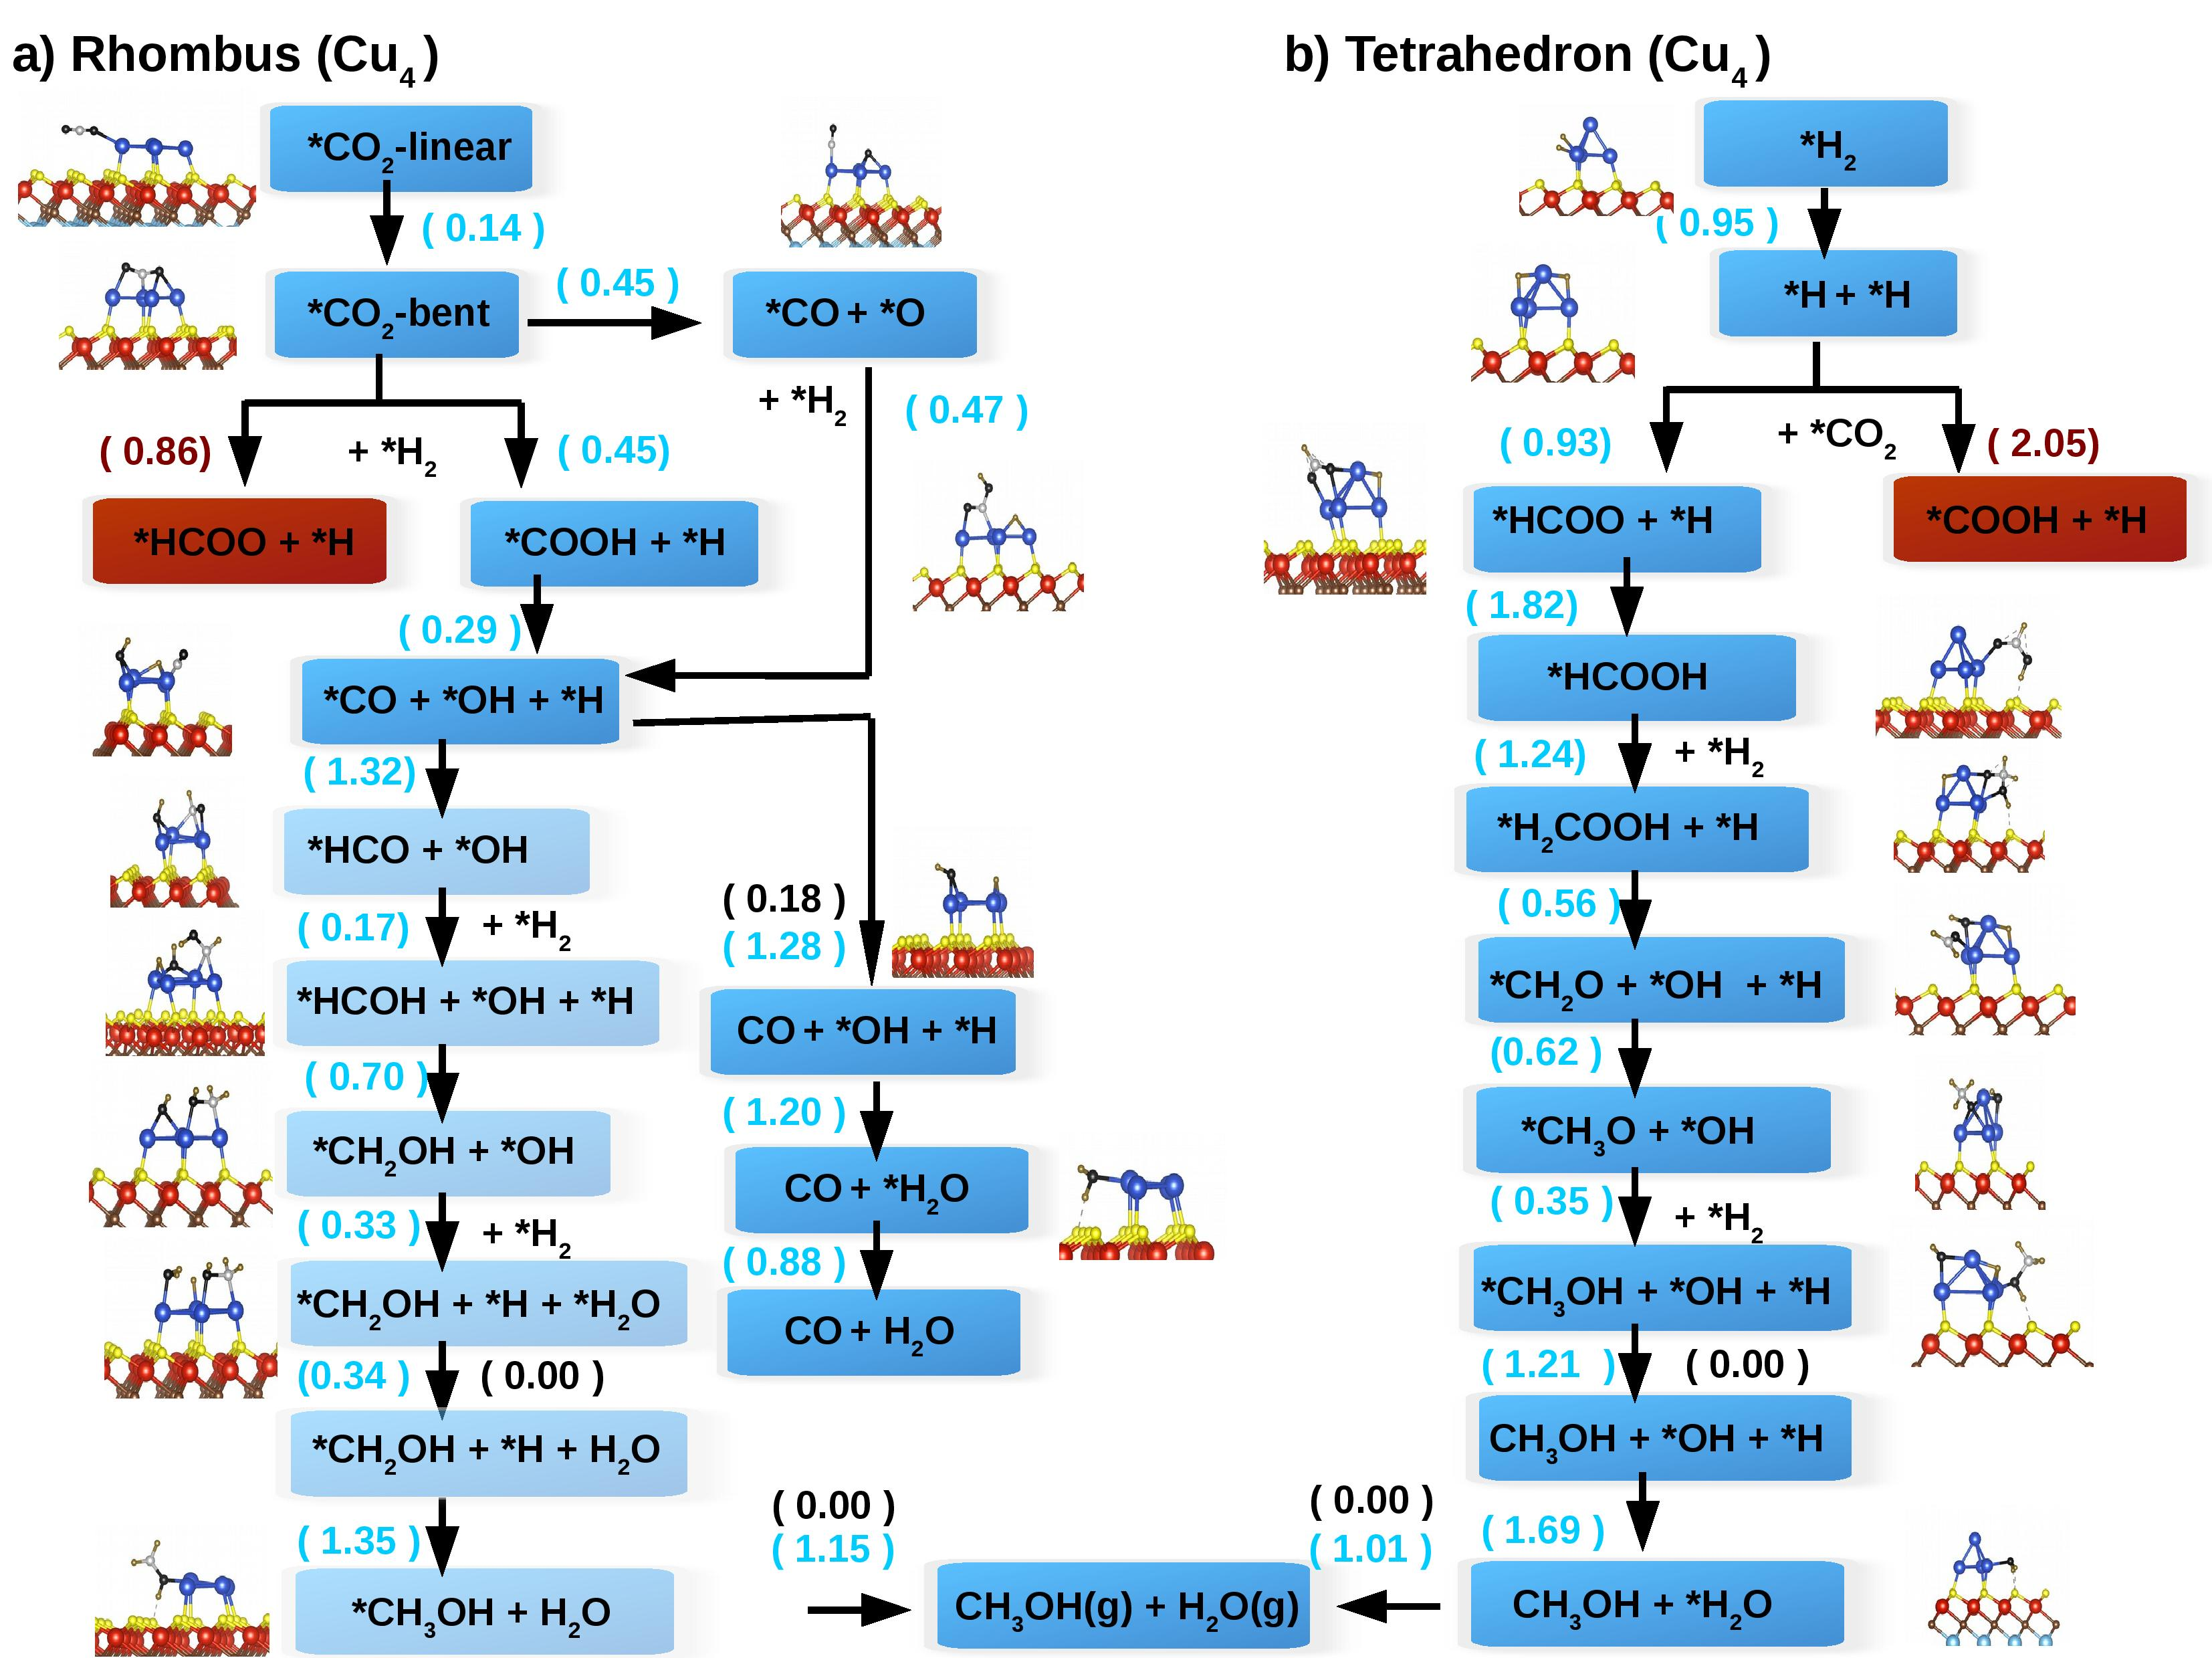
\includegraphics[width=14cm]{./Appendix3/figures/fig04.jpg} \\[0cm]
    \end{array}$
 \end{center}
 \caption{Flowchart for the conversion of CO$_2$ to CH$_3$OH for (a) rhombus (b) tetrahedron Cu$_4$/Ti$_2$CO$_2$. The blue boxes with blue arrows represent the intermediates for the most probable (primary) route. The red boxes, on the other hand, are the intermediates which need higher activation energy compared to the intermediates in the blue boxes. Therefore, the formation probability of the intermediates in red boxes is comparatively lower and are thereof discontinued. The structure of the intermediates corresponding to the blue boxes are also provided. Values in blue and red colours denote the activation energies in eV. Values in black text are entropy corrected desorption energy of stable molecules in eV where a value of 0.00 signifies barrier less desorption.}
  \label{fig:04}
\end{figure}


\subsection{Comparing CO\texorpdfstring{$_2$}) reduction on rhombus and tetrahedral geometries of the copper tetramer}

From our results, we observe that the full hydrogenation of CO$_2$ is possible on both the tetramer geometries. However, each geometry selectively generates its product. In the case of rhombus tetramer, CO formation via the ``r-WGS" pathway is the most abundant product whereas on the tetrahedron, HCOOH formation via the ``FORMATE" pathway becomes the major product. . Therefore, a correlation between the shape/morphology of the cluster influences the the primary product and the underlying pathway. Moreover, we looked into previous literature reports on CO$_2$ reduction over copper tetramers supported on different substrates.   

Al$_2$O$_3$ supported Cu$_4$ cluster\cite{liu2015carbon} has a rhombus geometry and remains vertical on the surface such that only two coppers atoms (positively charged) are bound to the support oxygen atoms and the other two (neutral) are away from the support. The formation of HCOO and COOH is facilitated when H attacks CO$_2$ directly from the support. Both the processes are exothermic but needs an activation of 0.18 eV for HCOO and 1.05 eV for COOH. The relative ease of formation of HCOO makes the CO$_2$ reduction to primarily follow the ``FORMATE" pathway. TiO$_2$(110) supported Cu$_4$ cluster\cite{tao2019best} has a similar geometry to the tetrahedral cluster in our study as three positively charged Cu atoms are bound to the surface oxygen atoms (each Cu atom to two oxygen atoms) and a neutral (fourth) Cu atom away from the surface. The CO$_2$ is activated (bent configuration) on the cluster and binds strongly (-0.85 eV) at the interface of the cluster and support. However, the direct dissociation of CO$_2$ to (CO + O) needs 1.63 eV of activation energy. Hydrogen atom (H) from the surface attacks the activated CO$_2$ to form HCOO and COOH. HCOO formation is exothermic (-0.48 eV) with an activation energy of 0.11 eV whereas COOH formation is endothermic (0.19 eV) and needs 0.61 eV of activation energy. Therefore, ``FORMATE" pathway is also the preferred route for CO$_2$ reduction on Cu$_4$/TiO$_2$(110). $\beta$-Mo$_2$C(001) supported Cu$_4$\cite{posada2016conversion} is flat and has rhombus shape on the support similar to our rhombus tetramer. The activated CO$_2$ has a binding energy of -0.14 eV on the tetramer. The reaction of activated CO$_2$ with H to form COOH needs less activation energy (0.36 eV) than HCOO (0.46 eV) but the formation of COOH is found to be endothermic. The endothermic nature leads to the back dissociation of COOH to (*CO$_2$ + *H). The direct dissociation of CO$_2$ to form  (*CO + *O) needs approximately 0.80 eV which is more than the energy needed for COOH and HCOO formation. Therefore, HCOO formation is more favourable and the ``FORMATE" pathway becomes the most probable. However, on the clean  $\beta$-Mo$_2$C(001) surface, ``r-WGS" pathway is favoured as CO$_2$ dissociation is highly exothermic and needs a smaller activation of 0.21 eV. In Table \ref{tab:01}, we report some of the copper based catalysts studied for CO$_2$ reduction.

\begin{table}[htbp!]

 \caption{Comparison of methanol synthesis on some relevant Cu based catalysts for the ``FORMATE" and ``r-WGS" pathway. rh and th correspond to the rhombus and tetrahedron geometry. }
 \label{tab:01}
 
  \begin{center}
\resizebox{\textwidth}{!}{   
    \begin{tabular}{| *{7}{c|}}
  
    \hline
      Catalysts & \multicolumn{1}{c|}{$E_{a}$ (eV)} & \multicolumn{1}{c|}{RDS} & \multicolumn{1}{c|}{T (K)} & \multicolumn{1}{c|}{P$_{CO_2}$ (bar)} & \multicolumn{1}{c|}{P$_{H_2}$ (bar)} & \multicolumn{1}{c|}{Ref}\\ \hline


Cu$_4$-rh/Ti$_2$CO$_2$ &&&&&& \\
``r-WGS" & 1.35 eV & *CO + *OH + *H $\rightarrow$ *HCO + *OH & ... & ... & ... & this work   \\ \hline
Cu$_4$-th/Ti$_2$CO$_2$ &&&&&& \\
``FORMATE" & 1.82 eV & *HCOO + *H  $\rightarrow$ *HCOOH   & ... & ... & ... & this work   \\ \hline


Cu$_4$/Al$_2$O$_3$ &&&&&& \\ 
``FORMATE" & 1.14 & *HCOO + *H $\rightarrow$ *HCOOH & 498 & 0.038 & 0.013 &\cite{liu2015carbon} \\
``r-WGS"  & 1.05 & *CO$_2$ + *H $\rightarrow$ *COOH &&&& \\ \hline

Cu$_4$/TiO$_2$(110) &&&&&& \\
``FORMATE" & 0.91 & *H$_2$CO + *OH + *H $\rightarrow$ *H$_3$CO + *OH & 400-700 & 0.25 & 0.75 &\cite{tao2019best} \\
``r-WGS"  & 0.61 & *CO$_2$ + *H $\rightarrow$ *COOH &&&&\\ \hline

Cu$_4$/$\beta$-Mo$_2$C(001) &&&&&& \\
``FORMATE" & 1.23 & *CH$_3$O + *H $\rightarrow$ *CH$_3$OH  & 500  & 40&10 &\cite{posada2016conversion} \\
 ``r-WGS"   & 0.36 &  *CO$_2$ + *H $\rightarrow$ *COOH   &&&&\\ \hline

Cu$_{29}$/ZnO(0001) &&&&&& \\
``FORMATE"  & 1.41 & *H$_2$COO + *H $\rightarrow$ *H$_2$CO + *OH & 500-600  & 0.51&4.56 &\cite{yang2010fundamental} \\
 ``r-WGS"  & 1.14 & *CO + *H + *OH $\rightarrow$ *CO + *H$_2$O &&&& \\ \hline

Cu(111) &&&&&& \\
 ``FORMATE"   & 1.23 & *HCOOH + *H $\rightarrow$ *H$_2$COO & 500  &... &... &\cite{zhao2011insight} \\
  ``r-WGS"     & 1.17 & *CO$_2$ + *H + *H $\rightarrow$ *COOH + *H &  & & & \\ \hline

%Cu(211)    & 1.32 &  HCOO +  H $\rightarrow$ HCOOH & 500  & 40 & 10 &\cite{behrens2012active} \\ \hline
%Cu(111)    & 0.99 & CH$_3$OH +  H +  OH $\rightarrow$ CH$_3$OH +  H$_2$O  & 500  & 40&10 &\cite{behrens2012active} \\ \hline
%Cu(111)    & 1.60 &  H$_2$COO +  H $\rightarrow$  H$_2$CO +  OH  & 500-600(E)  & 0.51(E)&4.56(E) &\cite{yang2010fundamental} \\ \hline
%CuZn(211)    & 1.37 &  HCOO +  H $\rightarrow$ HCOOH & 500  & 40 &10 &\cite{behrens2012active} \\ \hline
%Zn$_3$OH/Cu(111) & 1.28 &  HCOO +  H $\rightarrow$ HCOOH & 500  & 40&10 &\cite{reichenbach2018ab} \\ \hline
%Ni/Cu(001)    & 1.39 &  HCOO + (1/2)H$_2$ $\rightarrow$ CH$_2$OO  & ...  & ... & ... &\cite{yang2012theoretical} \\ \hline
%CuZn(211)    & 1.49 &  CH$_3$O +  H + H$_2$O $\rightarrow$  CH$_3$OH + H$_2$O & 525  & 4.6 & 0.5 &\cite{kattel2017active} \\ \hline
%ZnO/Cu(111)    & 0.90 &  HCOOH +  H $\rightarrow$  CH$_2$OOH  & 525  & 4.6 & 0.5 &\cite{kattel2017active} \\ \hline
%Pd(111)    & 1.09 &  CO +  H $\rightarrow$  HCO  & ... & ... & ... &\cite{brix2020tuning} \\ \hline
%PdZn(111)    & 0.90 &  H$_2$COOH $\rightarrow$  H$_2$CO +  OH & ... & ... & ... &\cite{brix2020tuning} \\ \hline

  \end{tabular}
} 
  \end{center}
\end{table} 

From the above discussion on Cu based catalysts, we conclude the choice of pathway is mostly dependent on the the extent of CO$_2$ activation and the ease with which C-O bond can be dissociated. The vertically positioned rhombus cluster from Liu et al.\cite{liu2015carbon} and tetrahedral cluster in this work do not facilitate exothermic CO$_2$ activation and follows the ``FORMATE" pathway. Although the tetramer clusters from Tao et al.\cite{tao2019best} (tetrahedral) and Posada et al.\cite{posada2016conversion} (rhombus) find favourable CO$_2$ activation, the dissociation of CO$_2$ to (*CO + *O) needs more energy than COOH and HCOO formation. Similar to the clean $\beta$-Mo$_2$C(001) surface, the rhombus cluster in our work find CO$_2$ dissociation exothermic with an activation barrier of 0.40 eV which is comparatively lower than that needed for hydrogenated products. Therefore, an ideal descriptor to understand the mechanism of CO$_2$ reduction is CO$_2$ activation and then its subsequent dissociation. A copper based catalyst not able to activate CO$_2$ but H$_2$ will follow the ``FORMATE" pathway. Catalysts which can favourably activate CO$_2$ needs to have a low C-O dissociation barrier (*CO + *O) compared to its hydrogenation in order to follow the ``r-WGS" pathway.   

\section{Conclusions}
\label{concle}
This study is an extension to our previous work in Appendix \ref{appendix2} where we investigated the role of geometry of supported copper tetramers on the activation of CO$_2$. Here, we explored the complete reaction profile for CO$_2$ hydrogenation to methanol on the two geometries (rhombus and tetrahedron) of Cu tetramers supported on O-terminated Ti$_2$C. The rhombus geometry is the most stable form in the gas phase whereas in the adsorbed state the tetrahedral geometry is the most stable. However, the energy needed to convert the less stable rhombus to more stable tetrahedron is higher than the CO$_2$ activation on the rhombus which ensures the availability of either forms on the Ti$_2$CO$_2$ support. It is observed that the more stable tetrahedral geometry due to its inability to activate the CO$_2$ follows the ``Formate" pathway for CO$_2$ reduction. On the other other hand, the rhombus geometry owing to its favourable CO$_2$ activation and dissociation, a consequence of lower stability, follows the ``r-WGS" pathway. Hence, in addition to temperature and cluster size effects, the morphology of the cluster also influences the product formation as formic acid becomes the major product from the tetrahedral tetramer whereas it is carbon monoxide from the rhombus geometry. 

\section{Supporting Information}

The following section contains the different reactions involved in the reduction of CO$_2$ on the supported tetramers (rhombus and tetrahedron). IS, TS, MS and FS in the figures refer to the initial state, transition state, metastable state and final state respectively. Relative energy values of the TS, MS and FS states, reported in the figures of this section are without ZPE corrections.

\begin{figure}[ht!]
  \begin{center}
    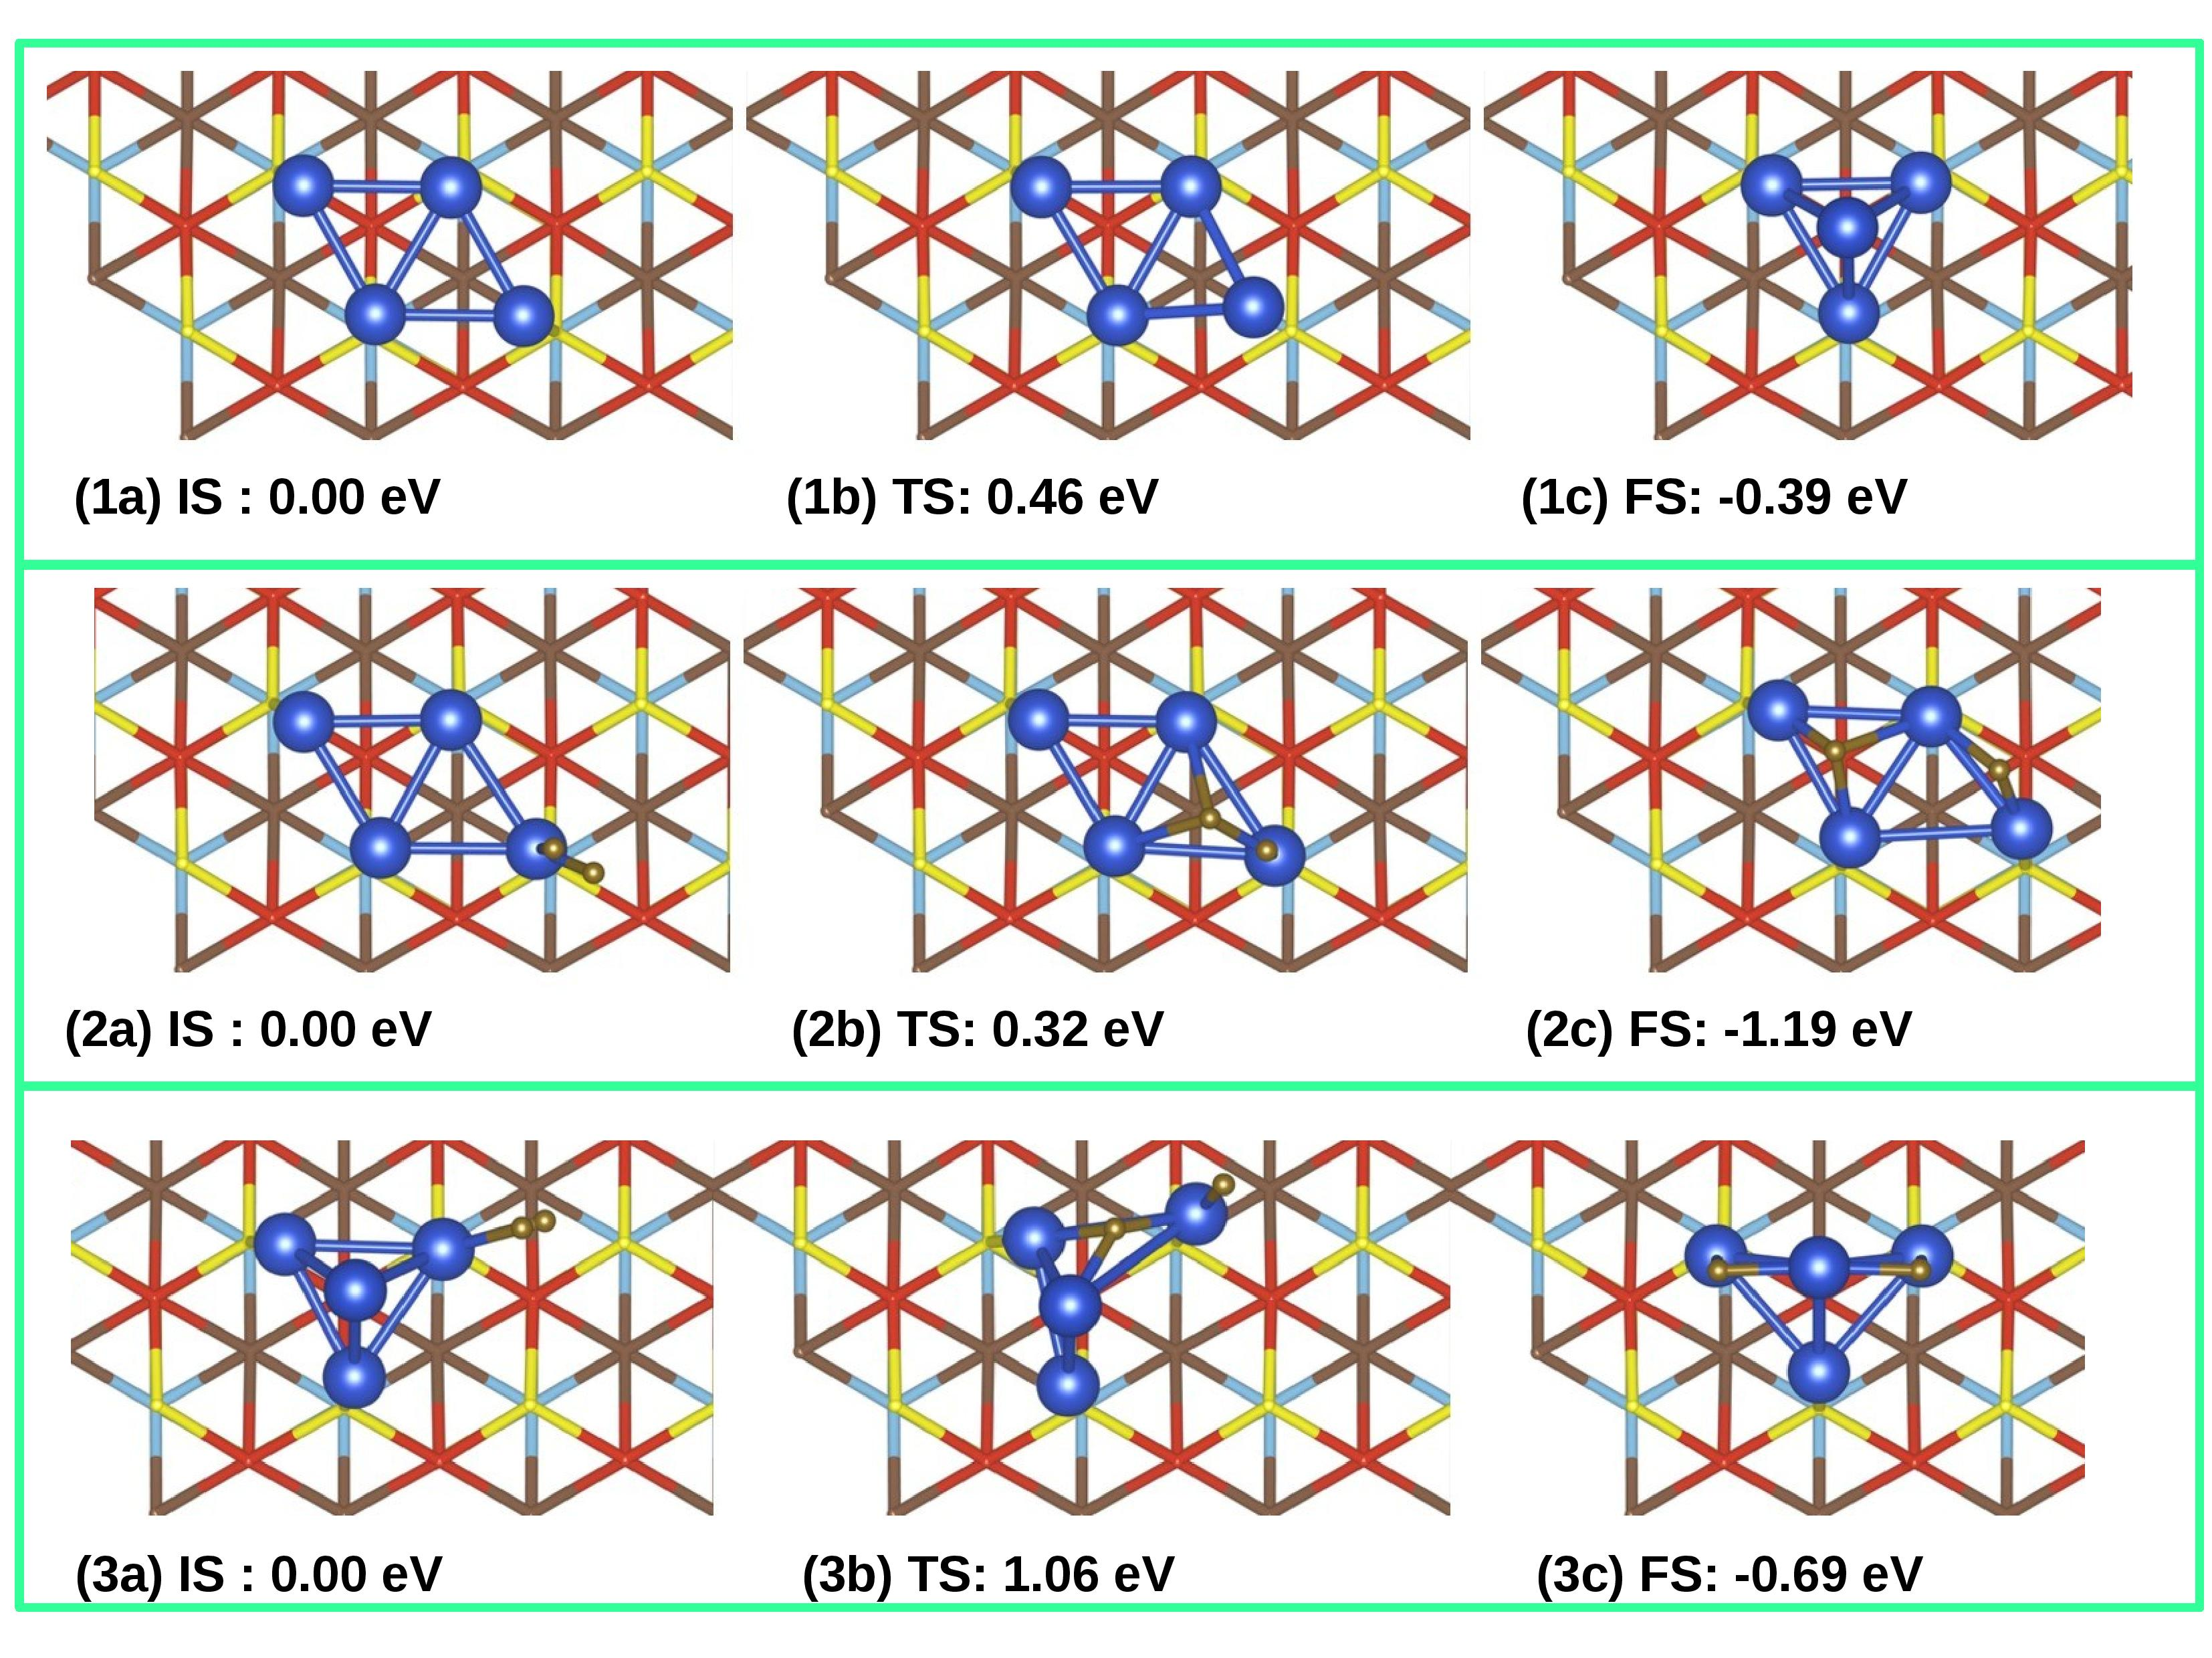
\includegraphics[width=0.9\textwidth]{./Appendix3/figures_si/p_101.jpg}
  \end{center}
    \caption{Reaction in top panel (1a-1c): Cu$_4$ (rhombus)/Ti$_2$CO$_2$ $\rightarrow$ Cu$_4$ (tetrahedron)/Ti$_2$CO$_2$. Reaction in middle (rhombus tetramer, 2a-2c) and bottom (tetrahedron tetramer, 3a-3c) panel: *H$_2$ $\rightarrow$ *H + *H. }
  \label{fig:si-101}
\end{figure}

\begin{figure}
  \begin{center}
    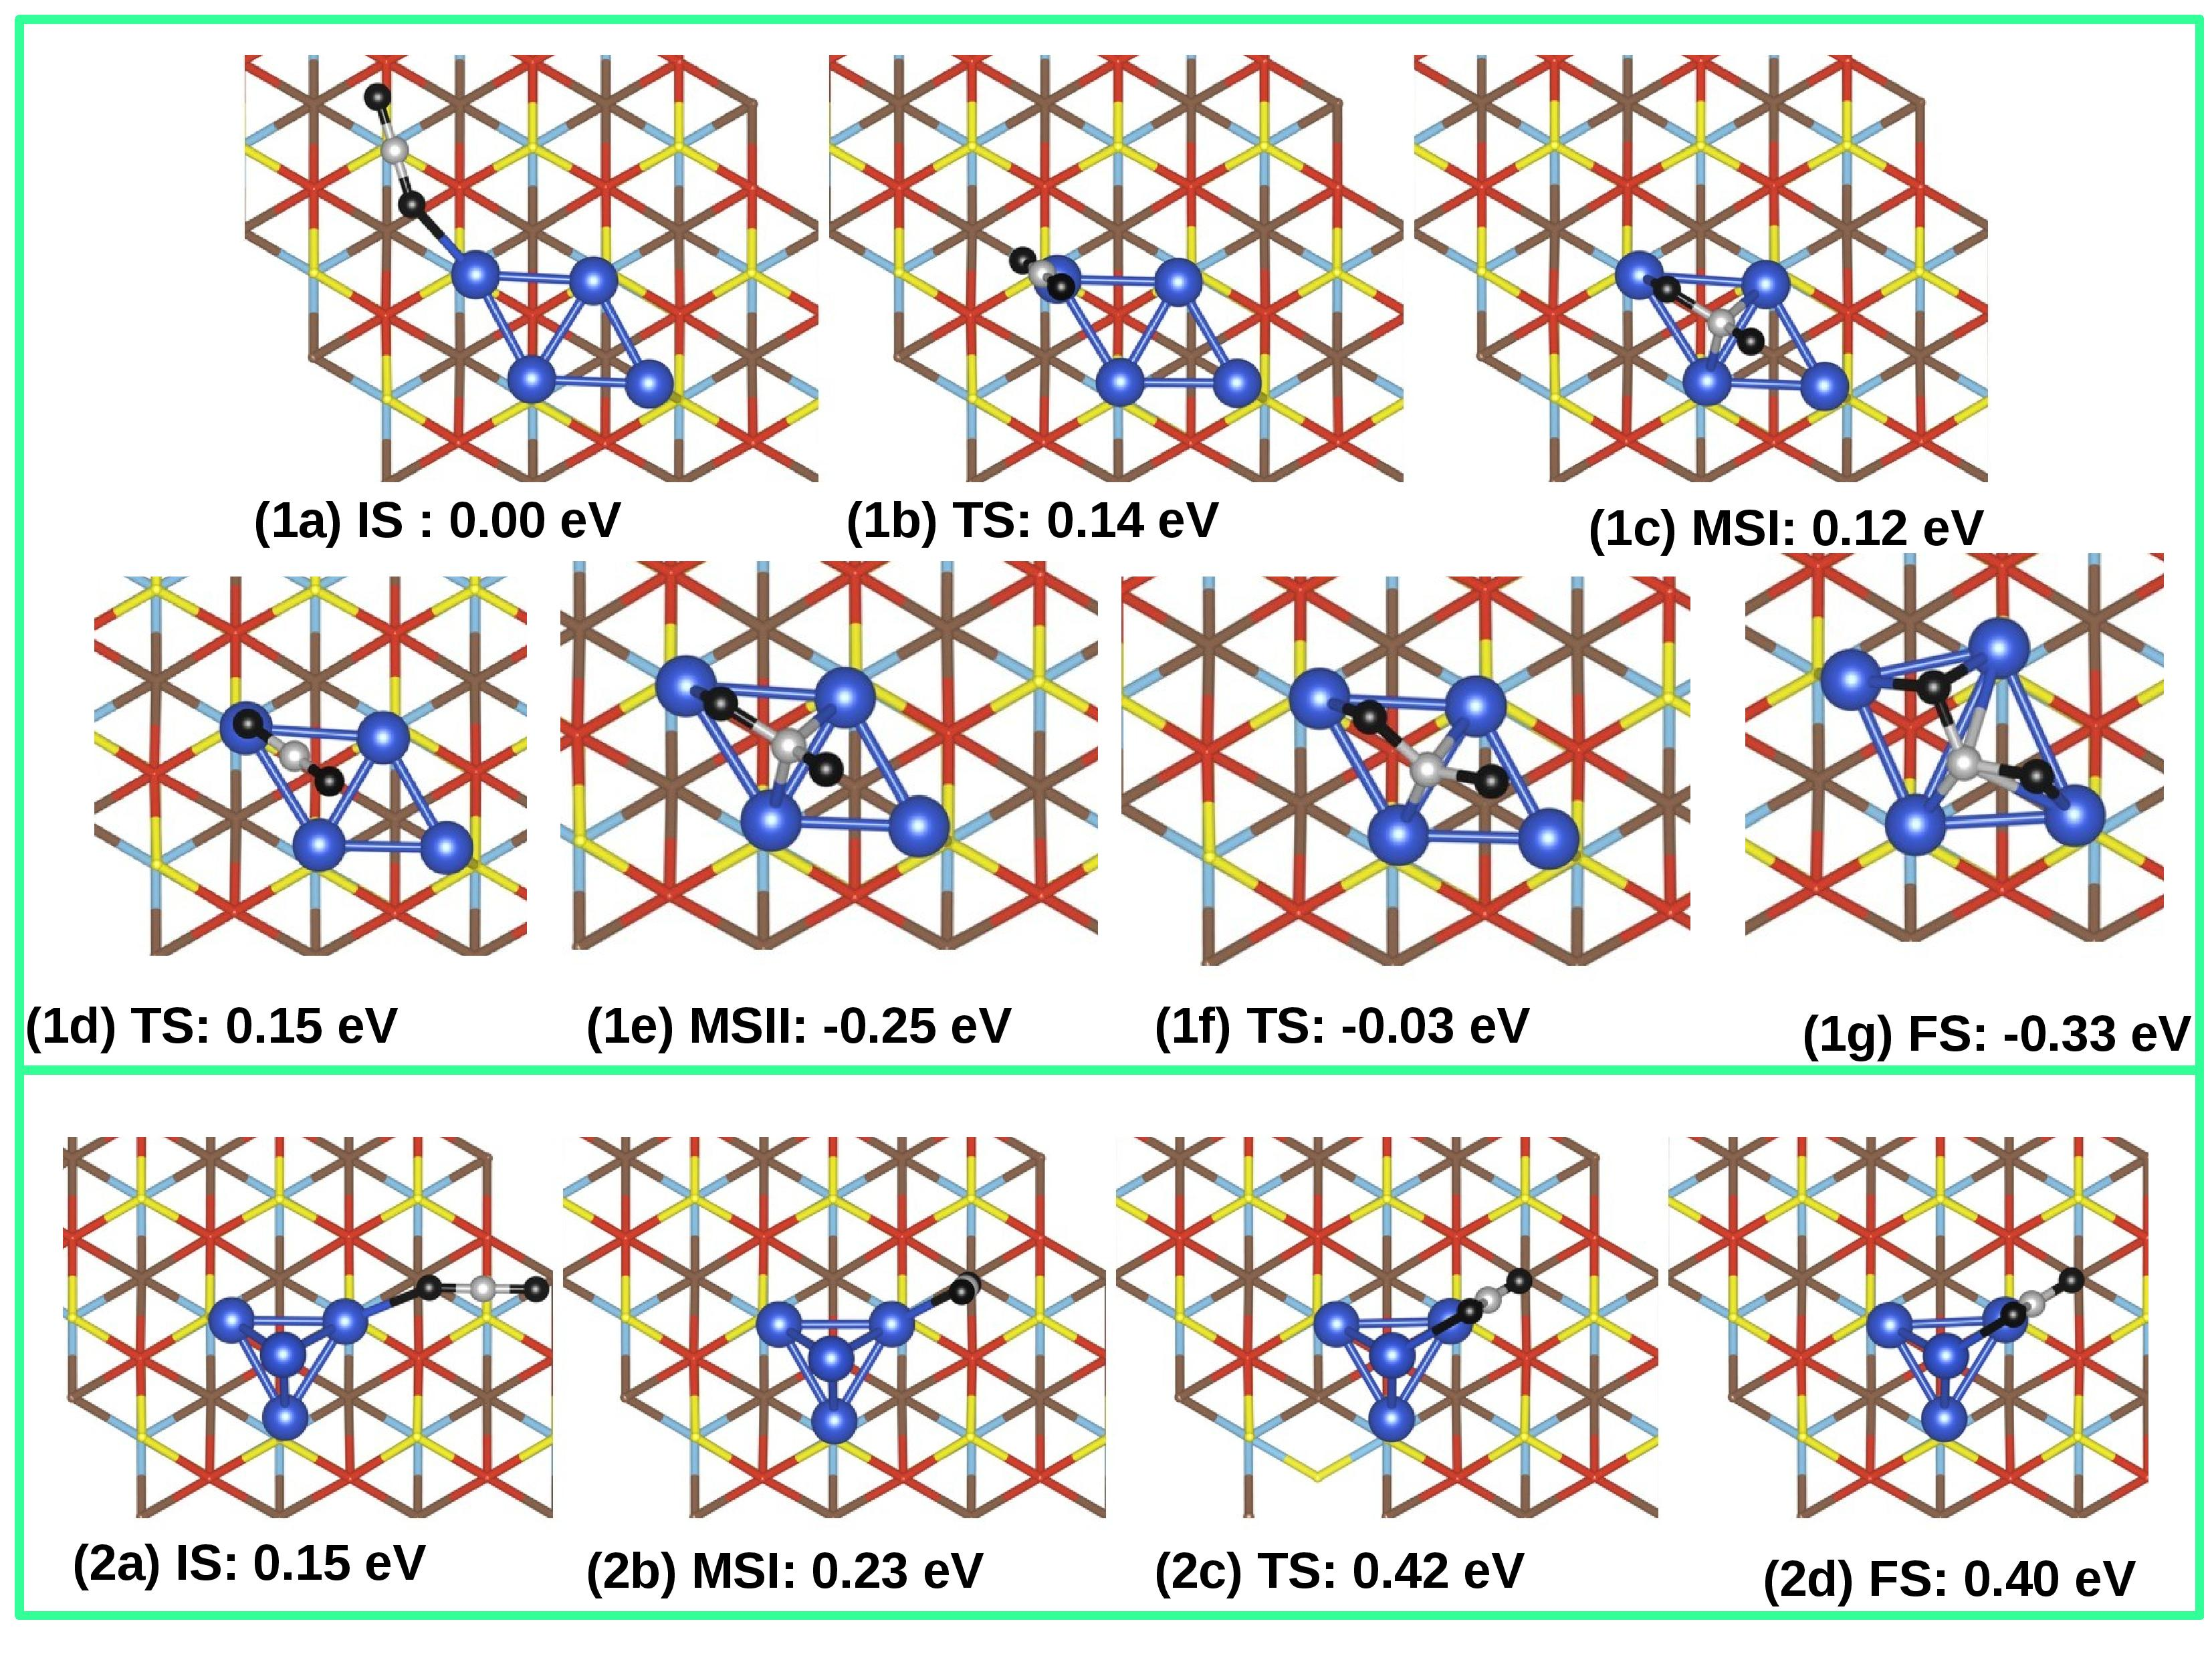
\includegraphics[width=0.9\textwidth]{./Appendix3/figures_si/p_102.jpg}
  \end{center}
    \caption{Reaction in top (rhombus tetramer, 1a-1g) and bottom (tetrahedron tetramer, 2a-2d) panel: *CO$_2$-linear $\rightarrow$ *CO$_2$-bent.   }
  \label{fig:si-102}
\end{figure}

\begin{figure}
  \begin{center}
    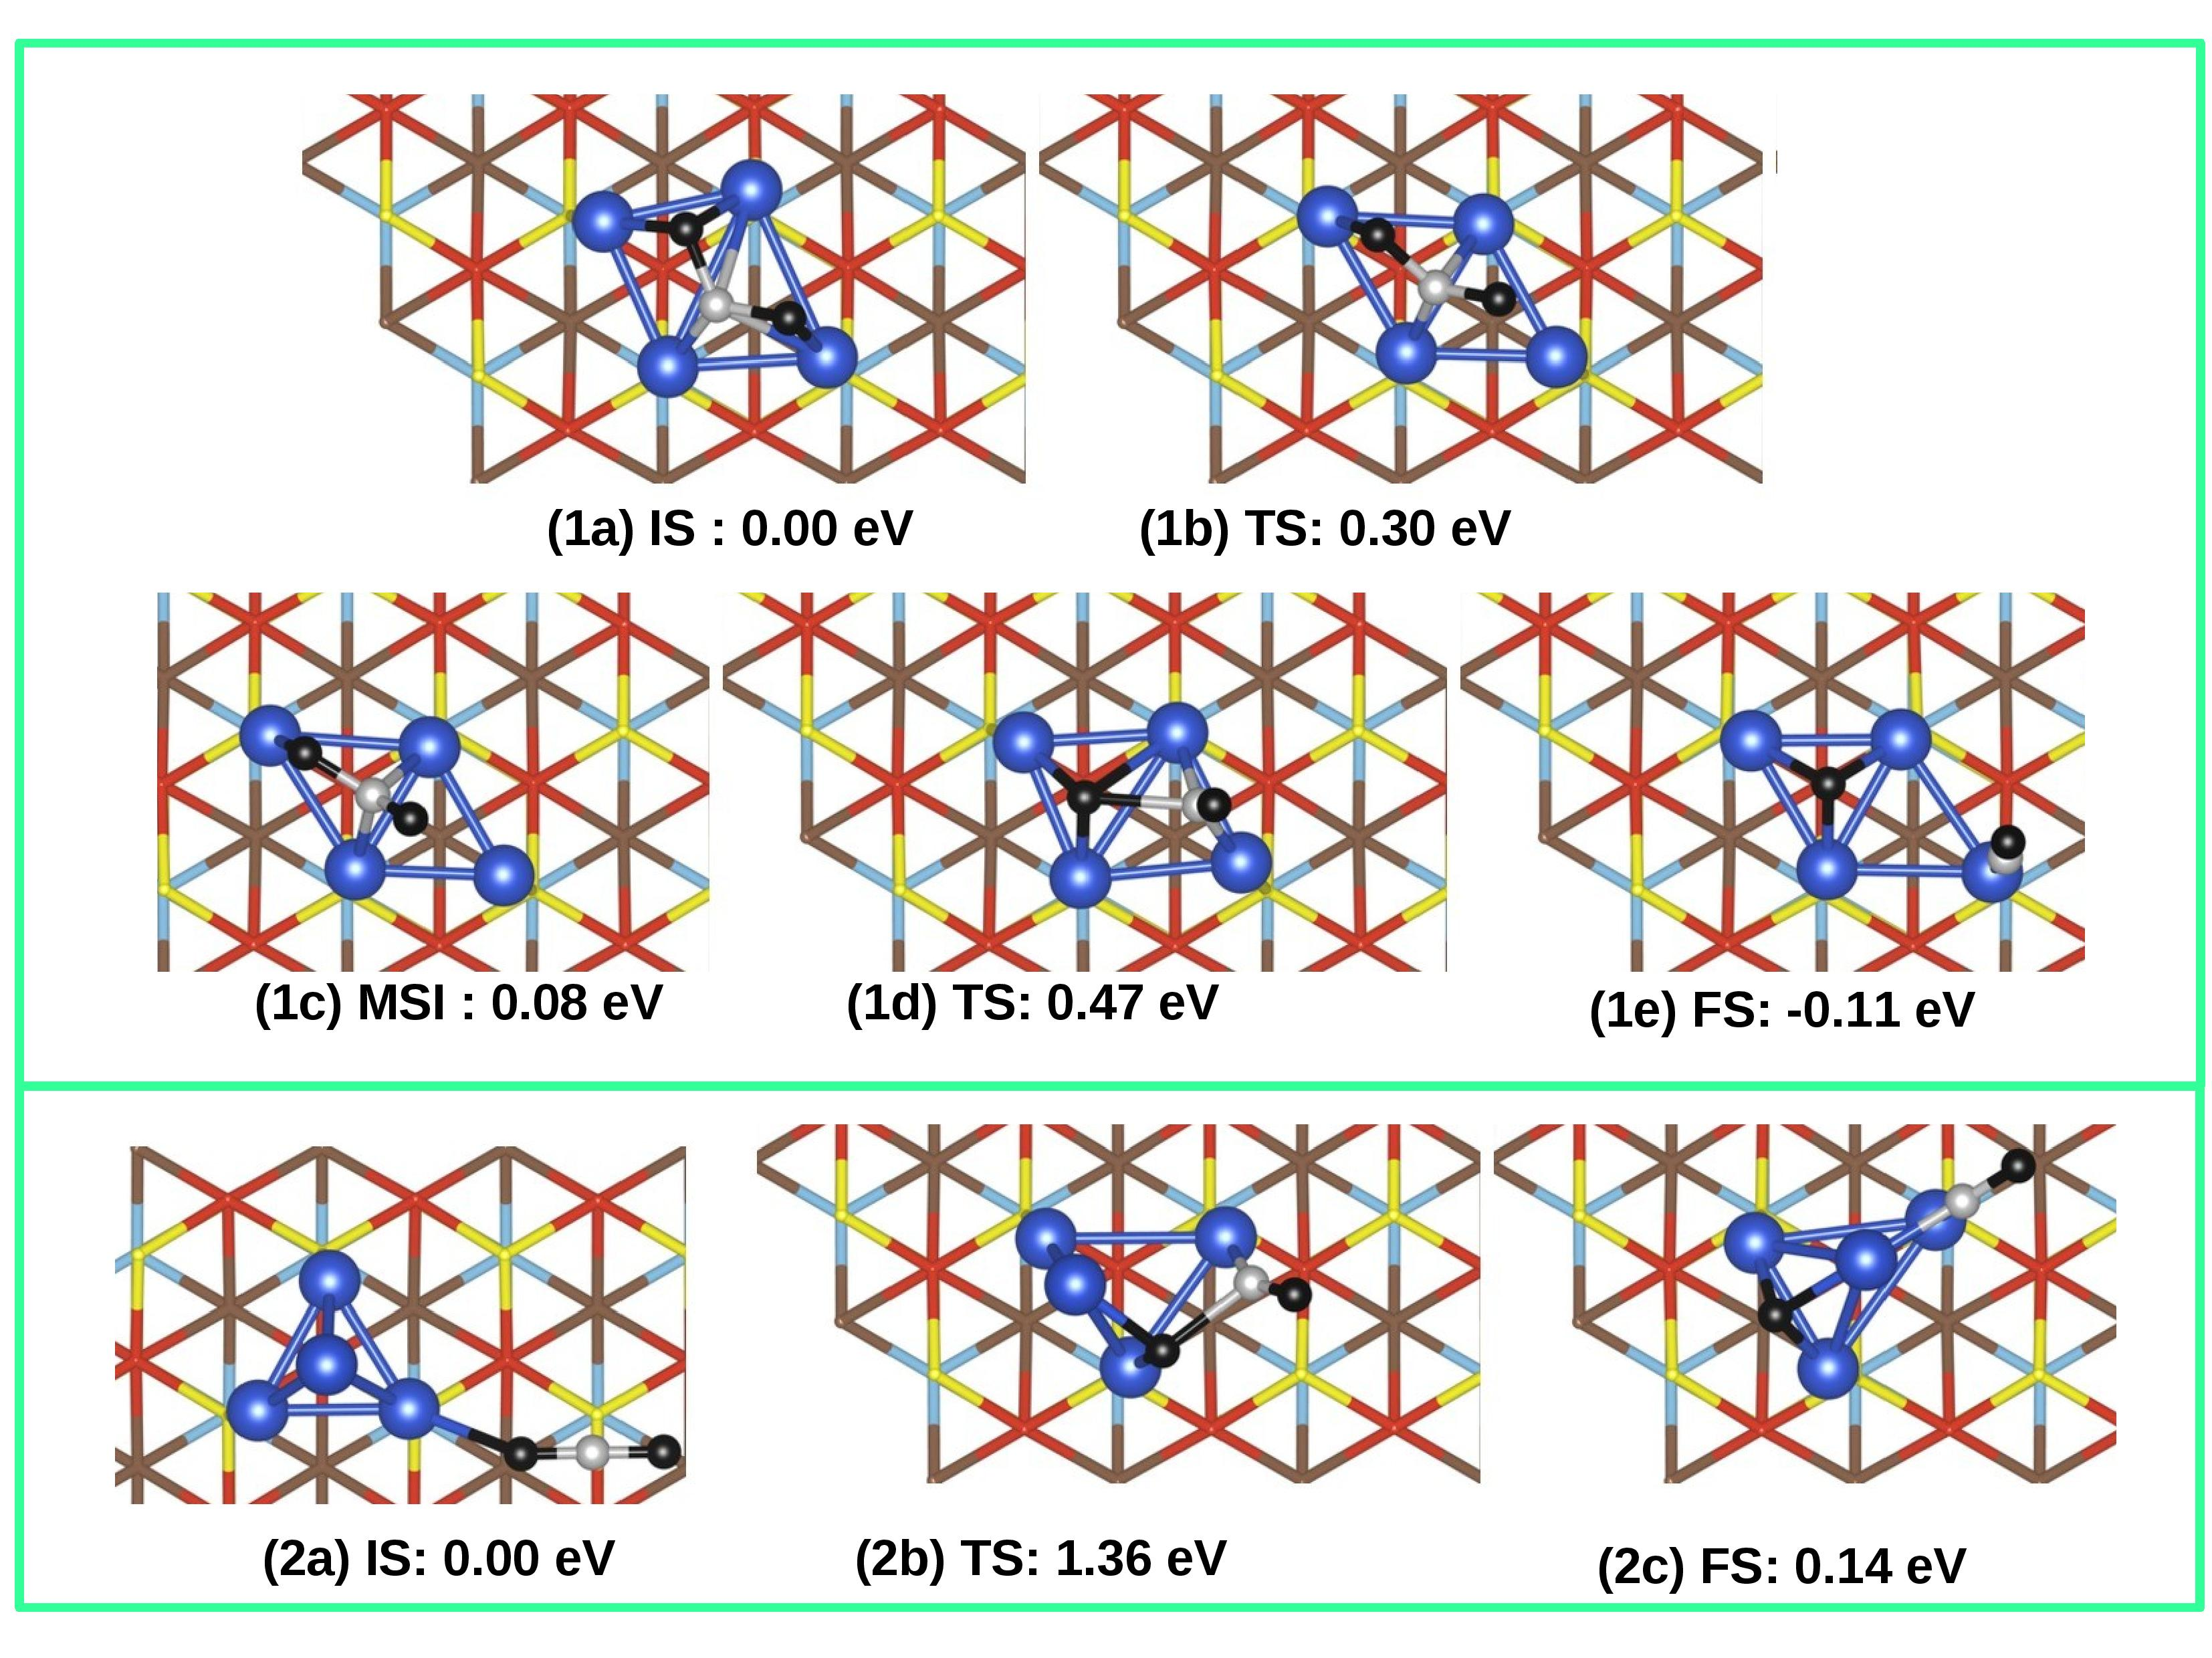
\includegraphics[width=0.9\textwidth]{./Appendix3/figures_si/p_103.jpg}
  \end{center}
    \caption{Reaction in top (rhombus tetramer, 1a-1e) and bottom (tetrahedron tetramer, 2a-2c) panel: *CO$_2$-bent $\rightarrow$ *CO + *O.   }
  \label{fig:si-103}
\end{figure}

\begin{figure}
  \begin{center}
    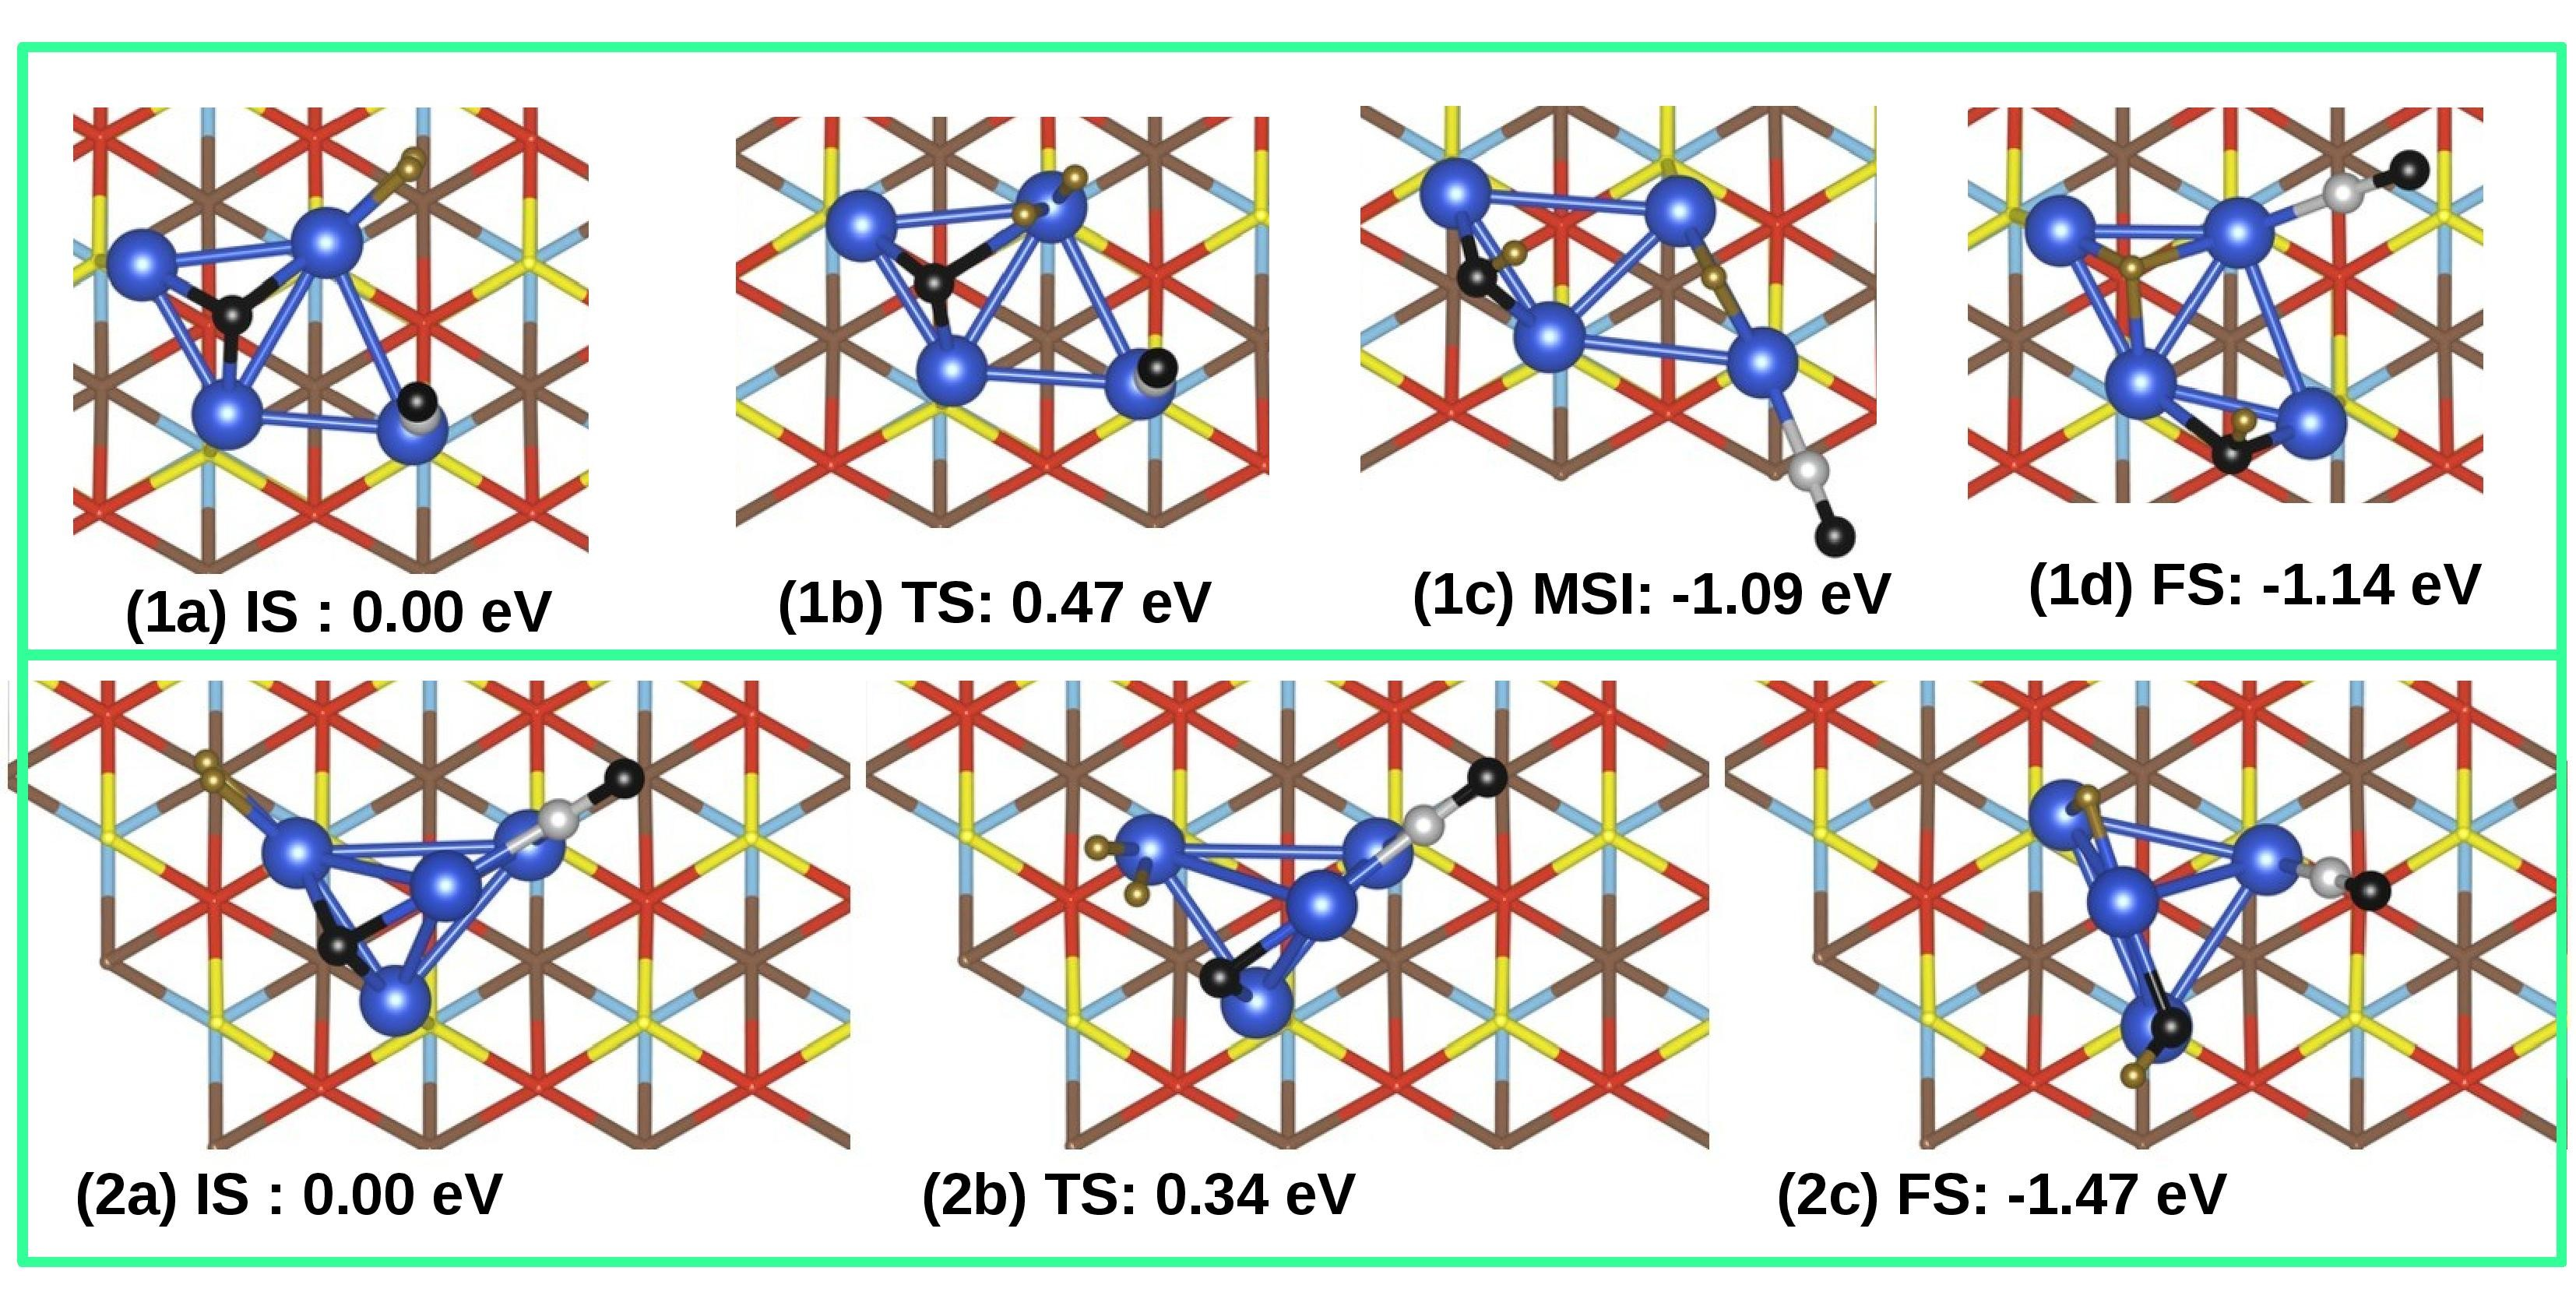
\includegraphics[width=0.9\textwidth]{./Appendix3/figures_si/p_104.jpg}
  \end{center}
    \caption{Reaction in top (rhombus tetramer, 1a-1d) and bottom (tetrahedron tetramer, 2a-2c) panel: *CO + *O + *H$_2$ $\rightarrow$ *CO + *OH + *H.   }
  \label{fig:si-104}
\end{figure}

\begin{figure}
  \begin{center}
    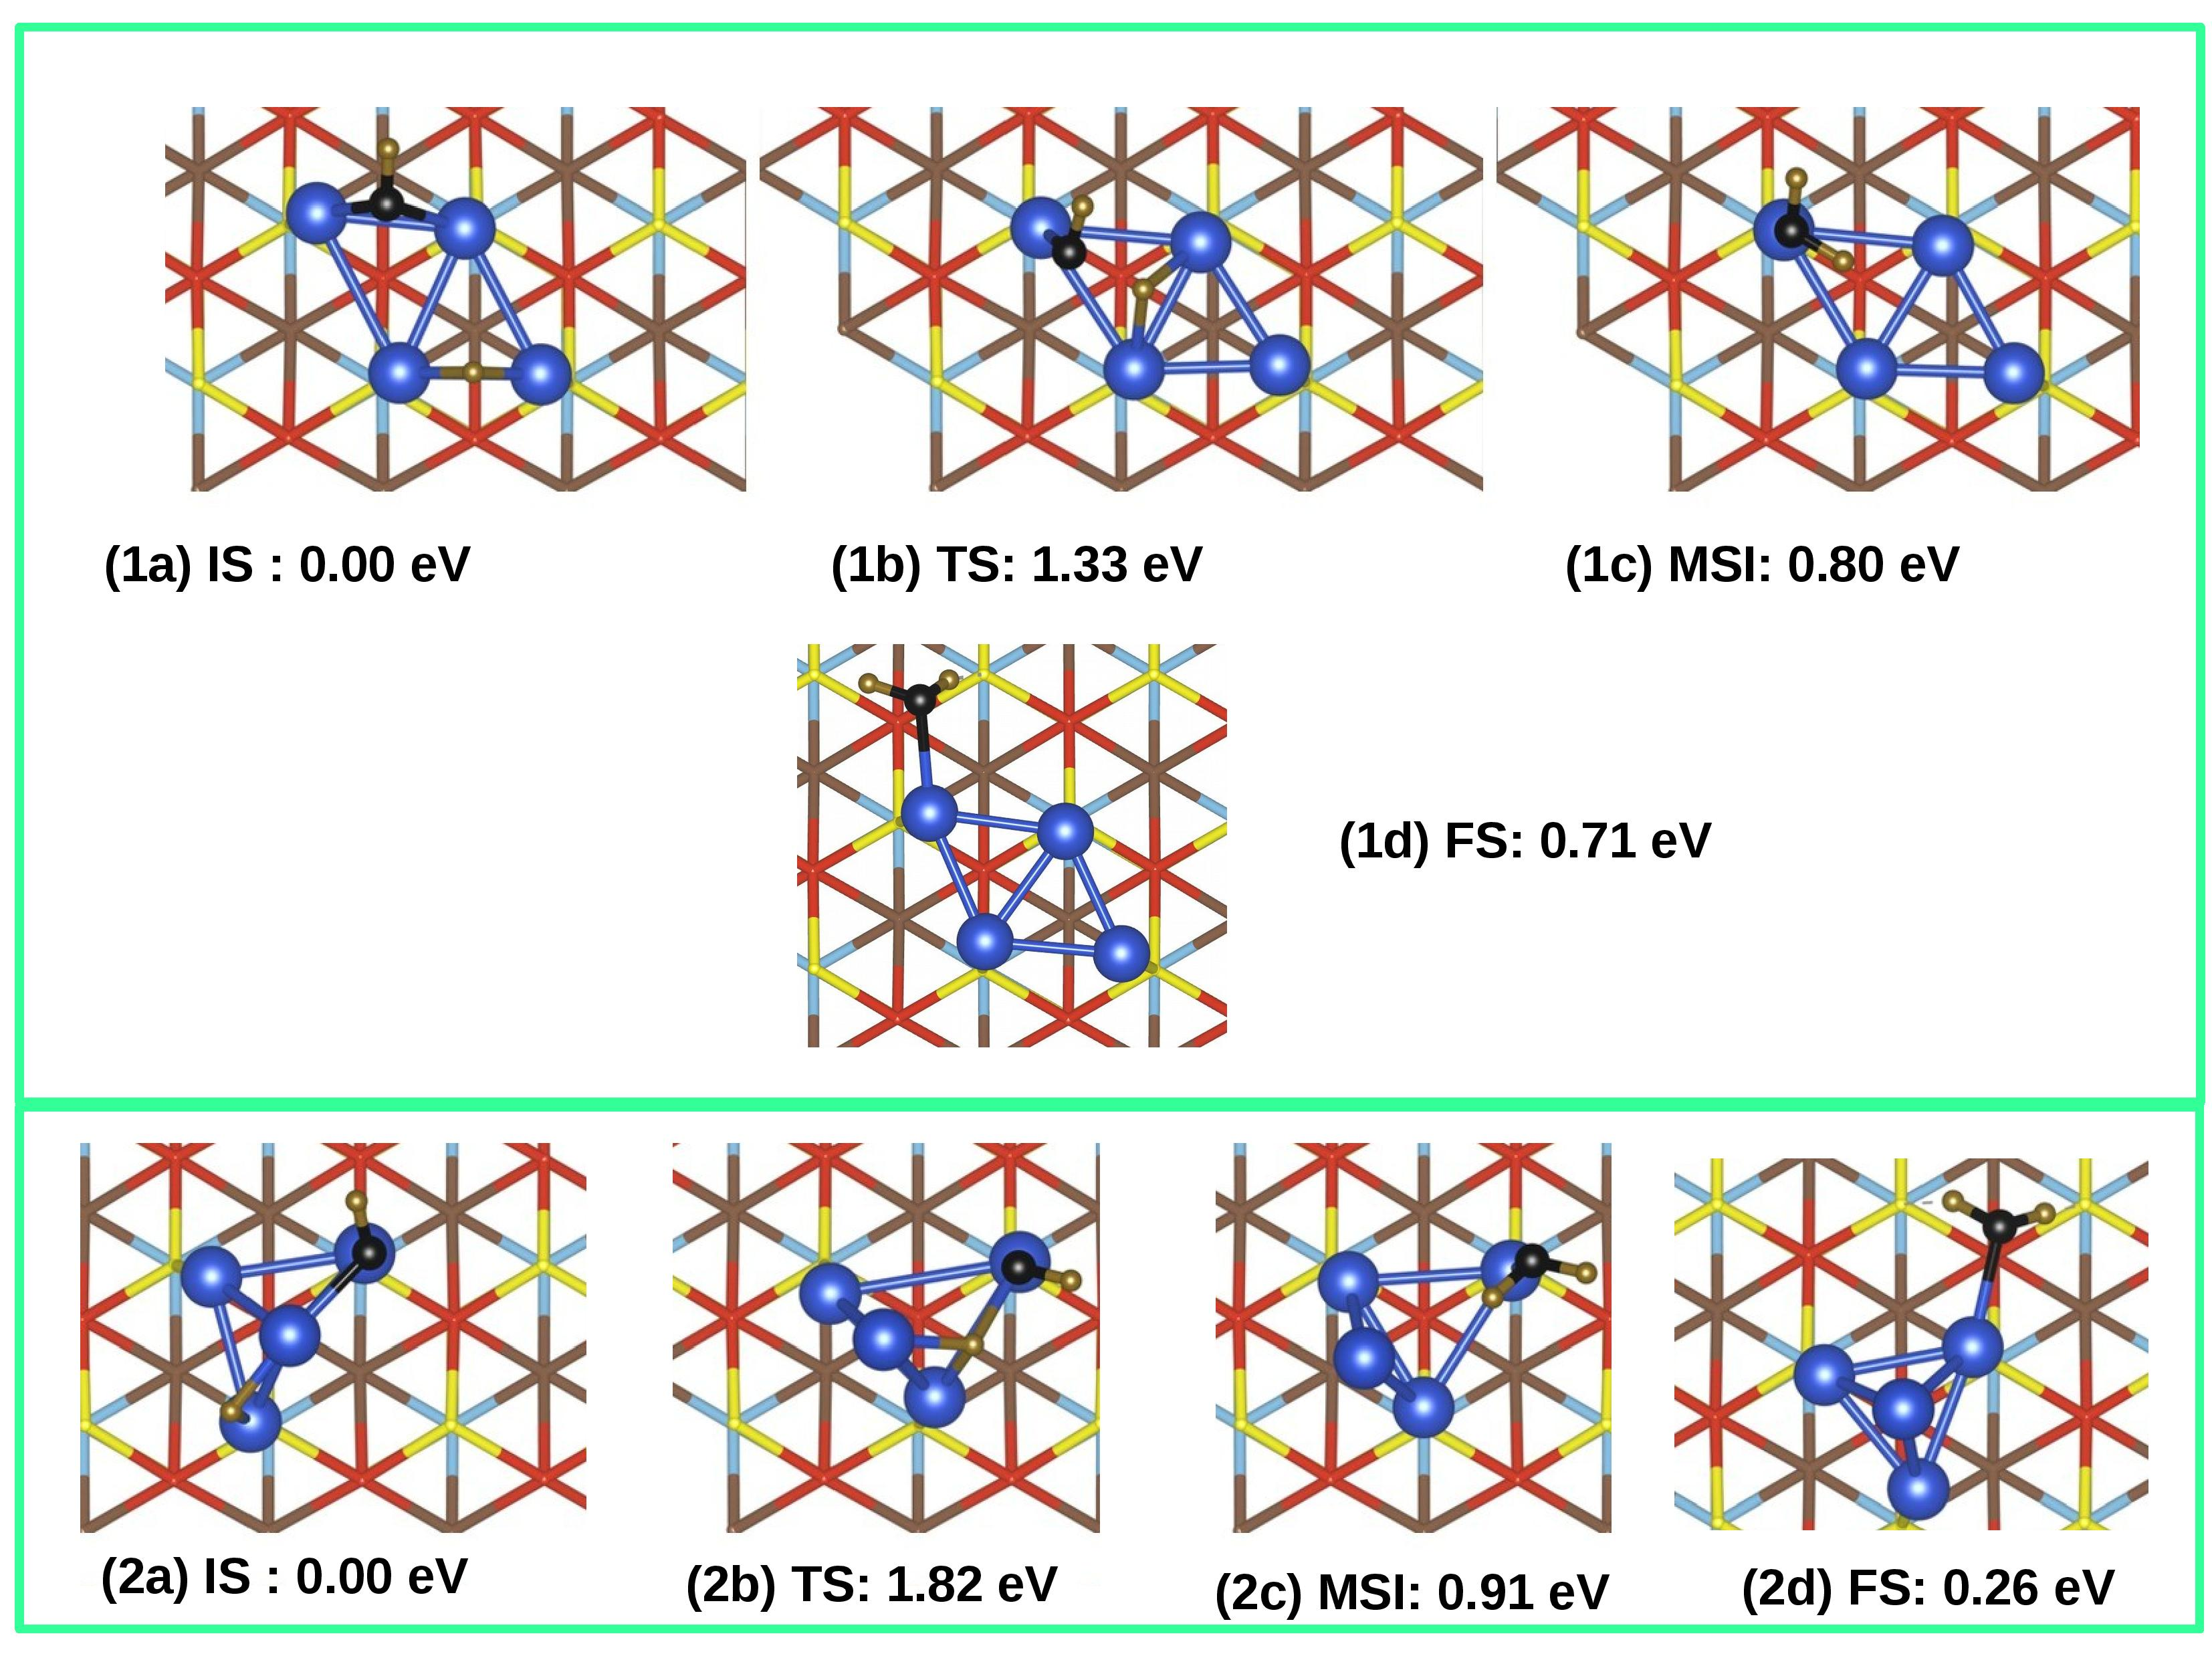
\includegraphics[width=0.9\textwidth]{./Appendix3/figures_si/p_105.jpg}
  \end{center}
    \caption{Reaction in top (rhombus tetramer, 1a-1d) and bottom (tetrahedron tetramer, 2a-2d) panel: *OH + *H $\rightarrow$ *H$_2$O.   }
  \label{fig:si-105}
\end{figure}

\begin{figure}
  \begin{center}
    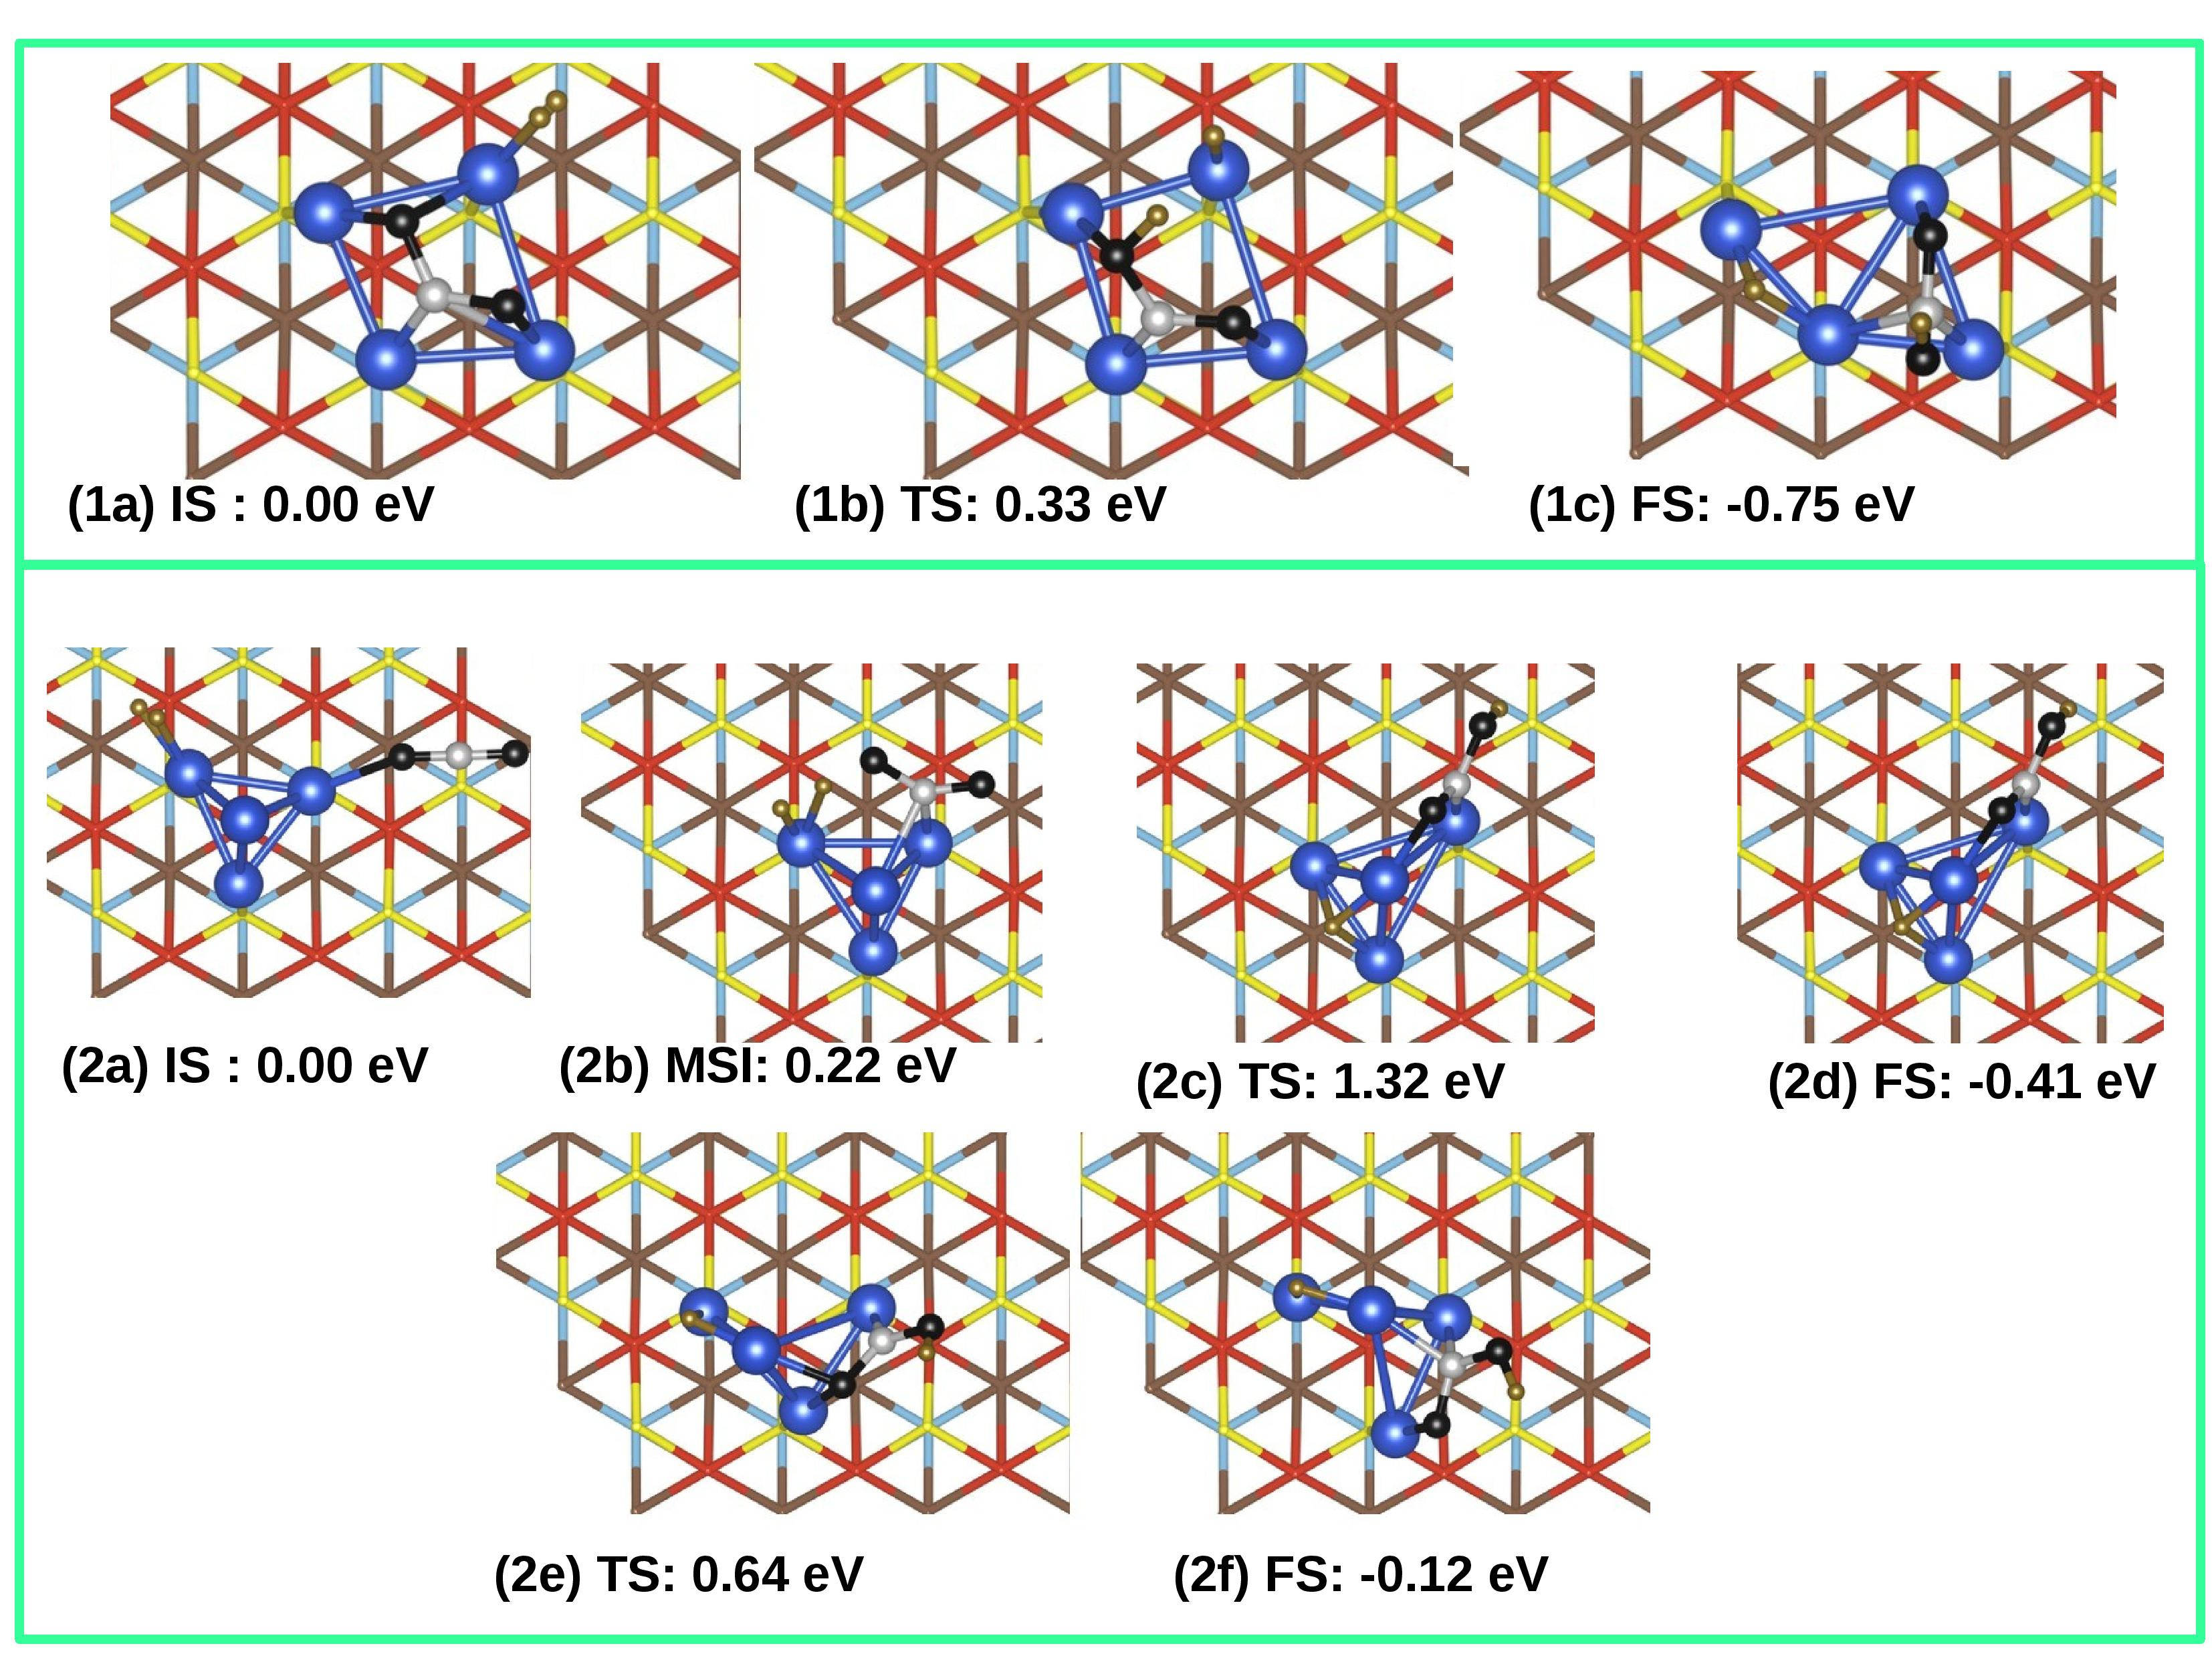
\includegraphics[width=0.9\textwidth]{./Appendix3/figures_si/p_106.jpg}
  \end{center}
    \caption{Reaction in top (rhombus tetramer, 1a-1c) and bottom (tetrahedron tetramer, 2a-2f) panel: *CO$_2$ + *H$_2$ $\rightarrow$ *COOH + *H.   }
  \label{fig:si-106}
\end{figure}

\begin{figure}
  \begin{center}
    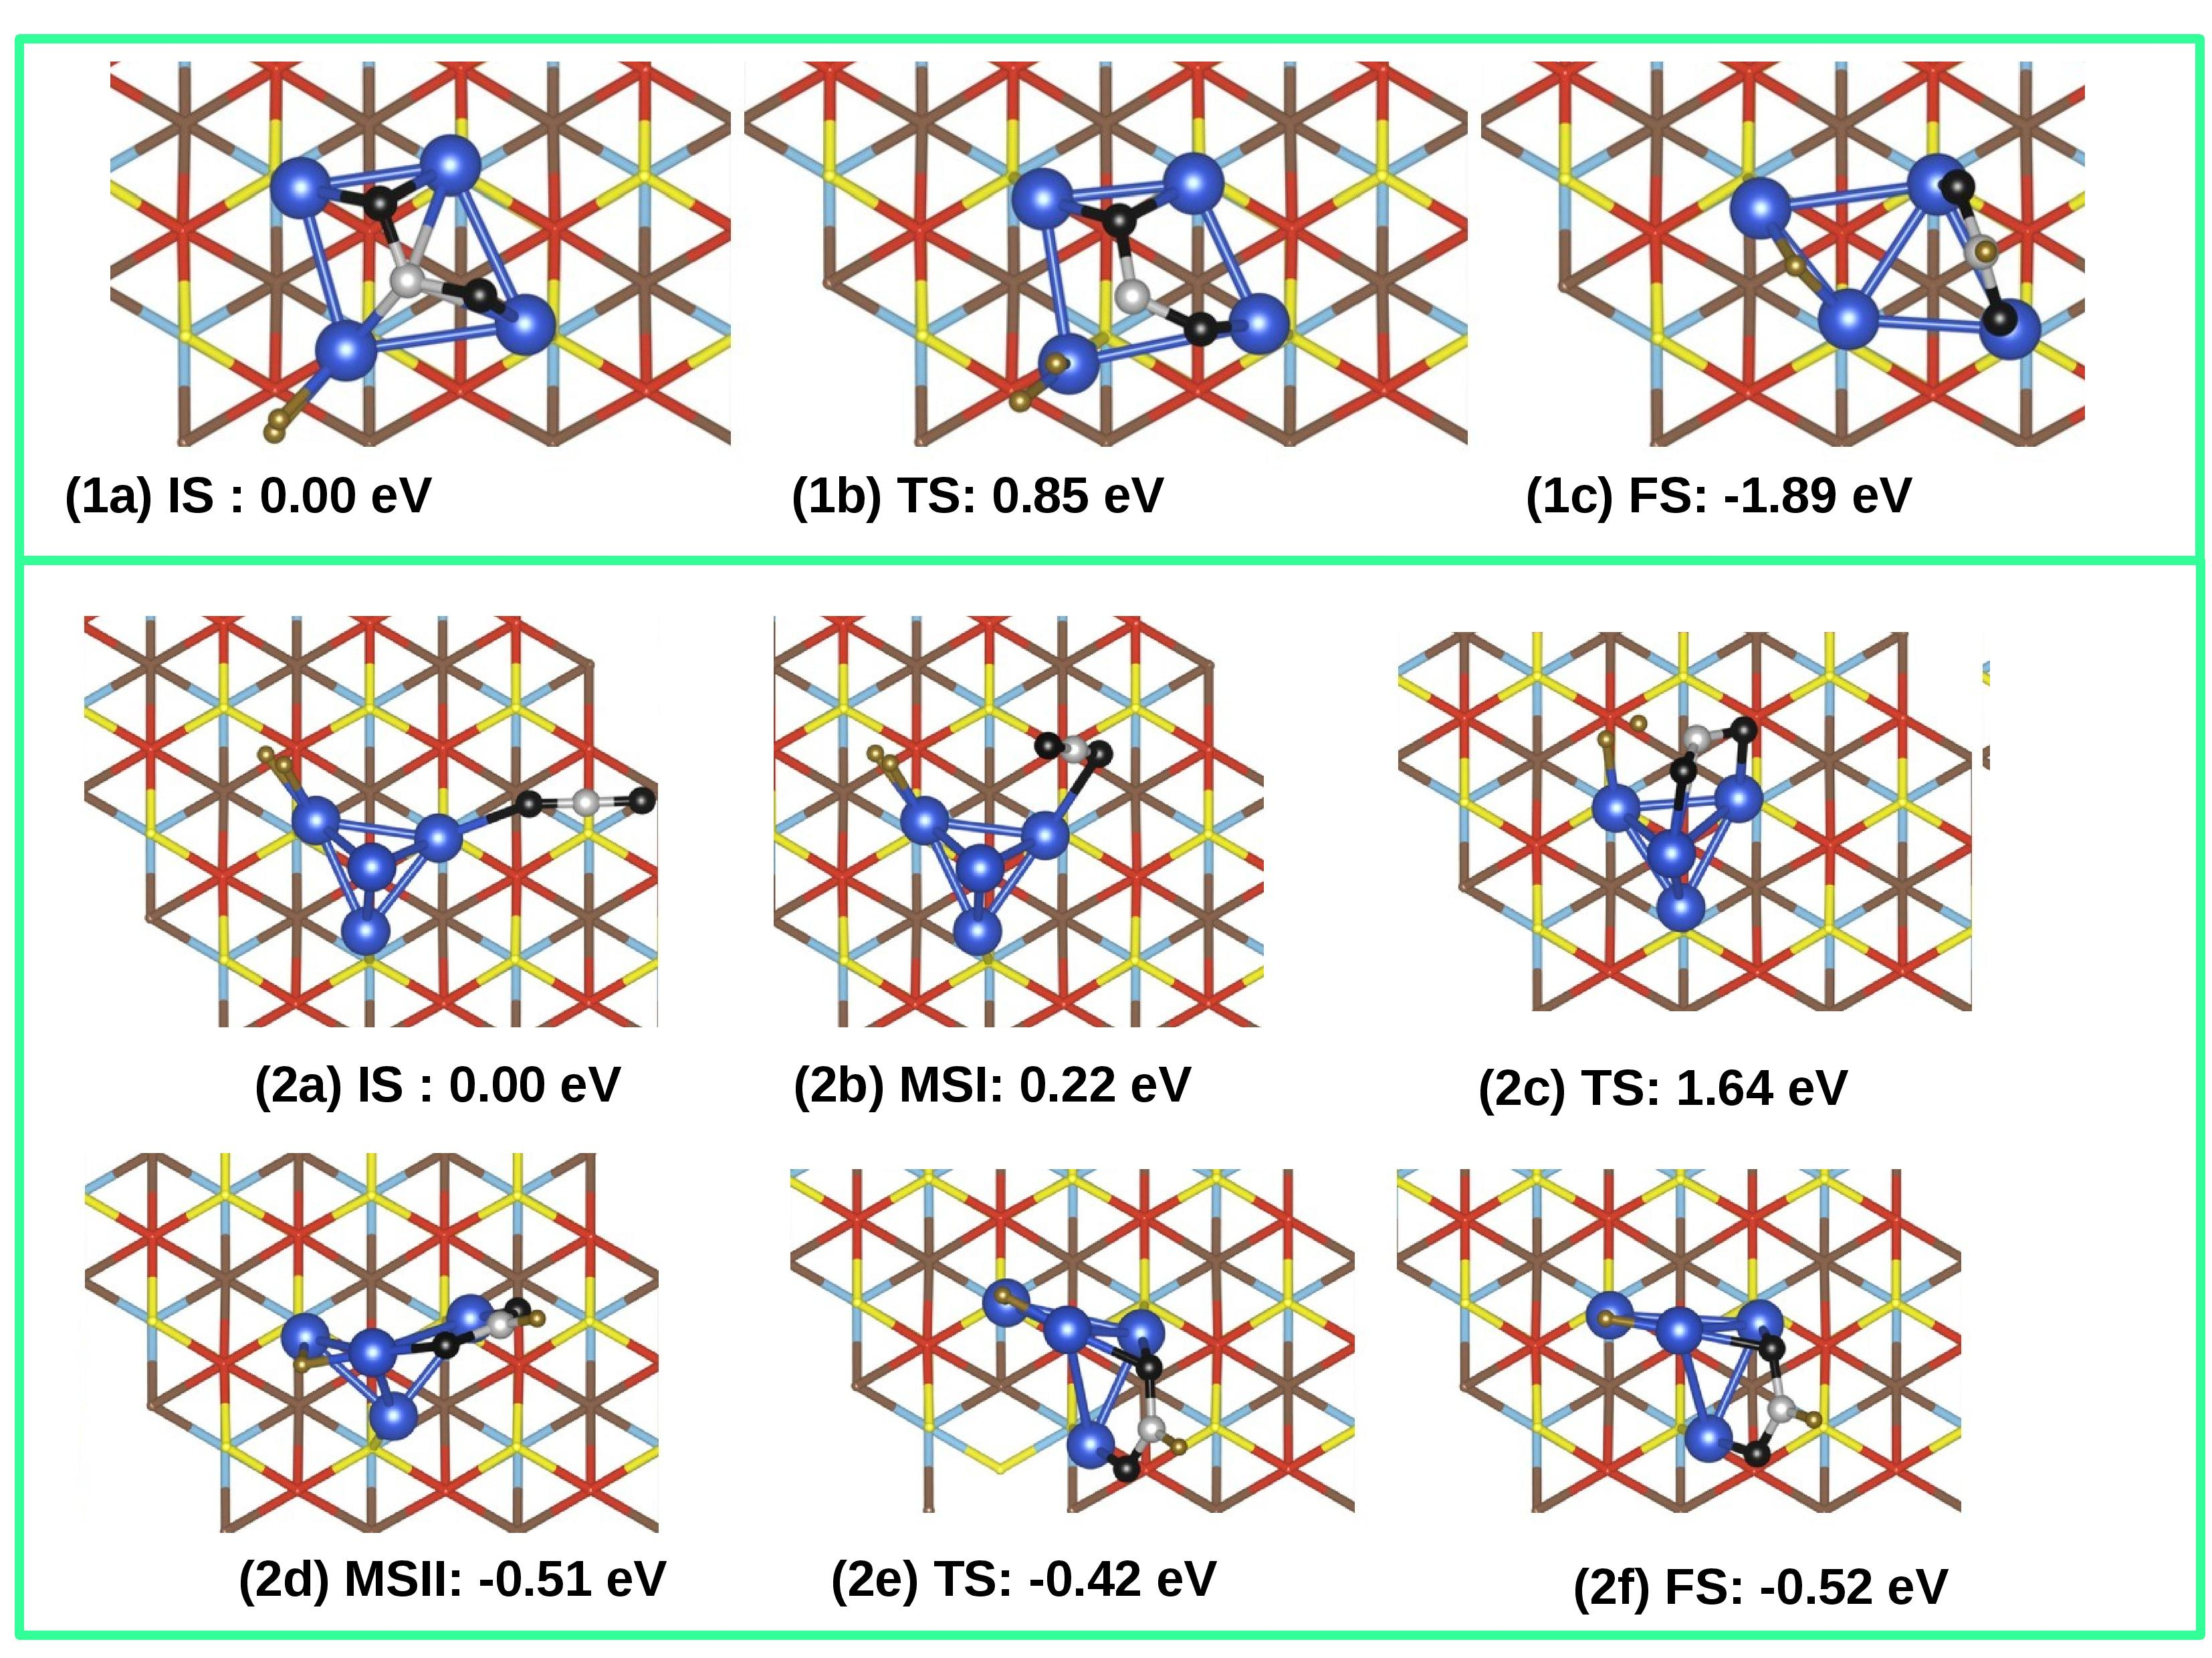
\includegraphics[width=0.9\textwidth]{./Appendix3/figures_si/p_107.jpg}
  \end{center}
    \caption{ Reaction in top (rhombus tetramer, 1a-1c) and bottom (tetrahedron tetramer, 2a-2f) panel: *CO$_2$ + *H$_2$ $\rightarrow$ *HCOO + *H.  }
  \label{fig:si-107}
\end{figure}

\begin{figure}
  \begin{center}
    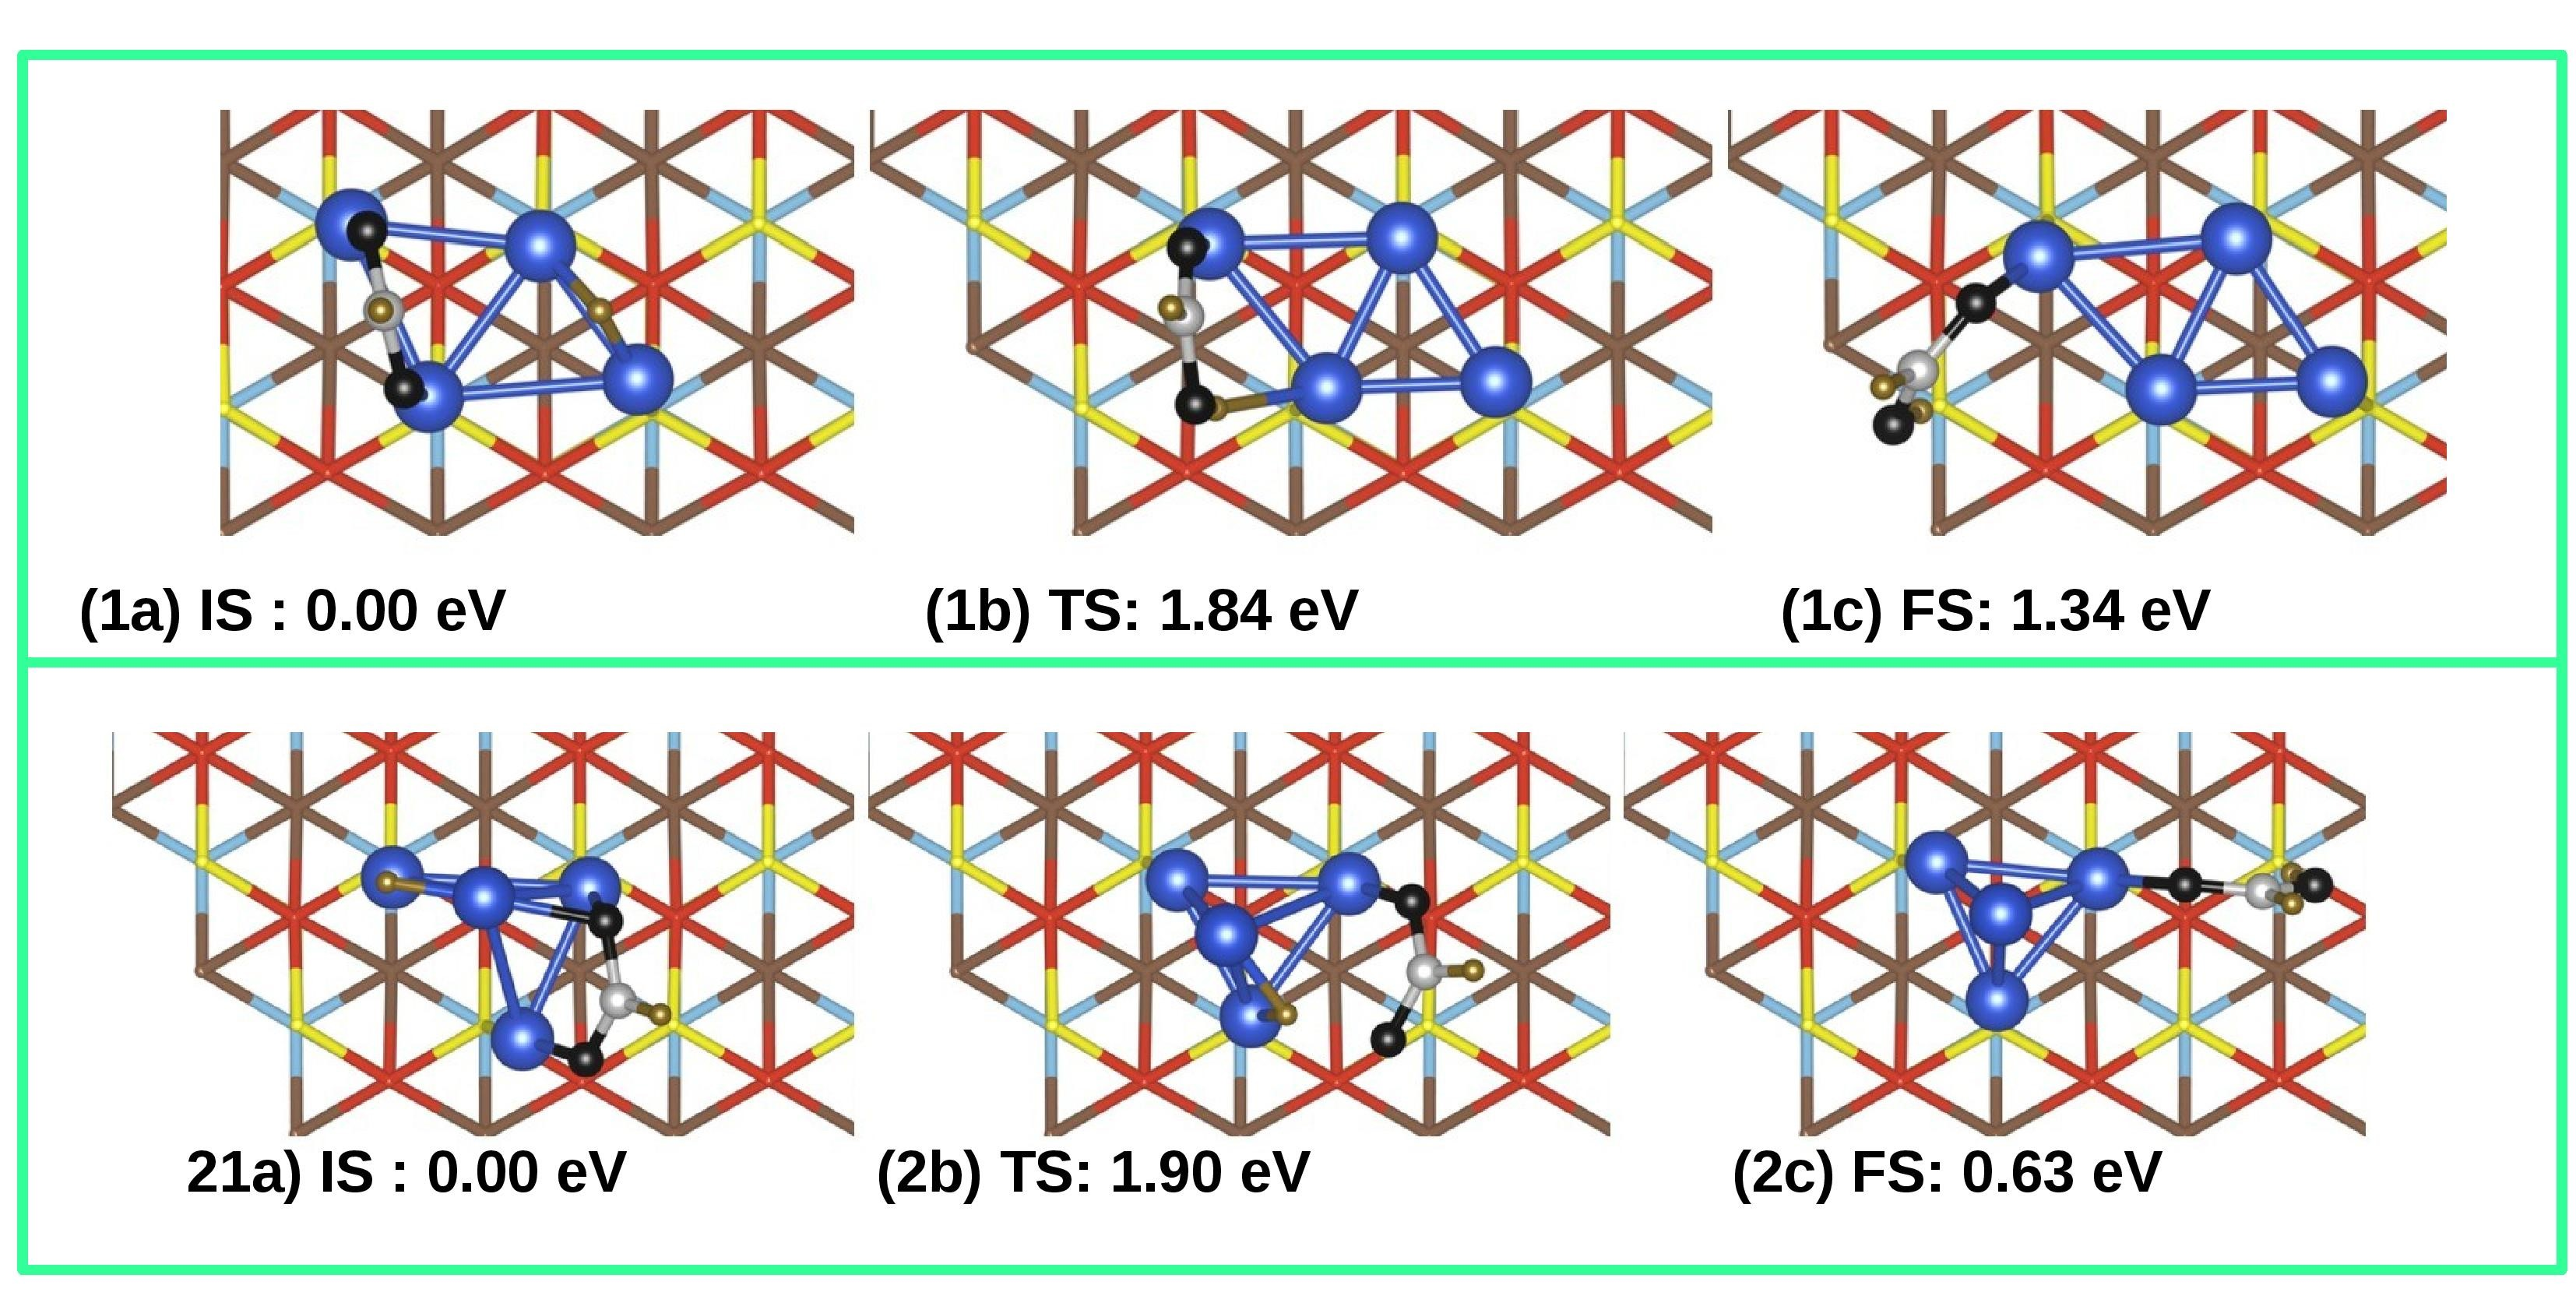
\includegraphics[width=0.9\textwidth]{./Appendix3/figures_si/p_108.jpg}
  \end{center}
    \caption{Reaction in top (rhombus tetramer, 1a-1c) and bottom (tetrahedron tetramer, 2a-2c) panel: *HCOOH + *H $\rightarrow$ *HCOOH.   }
  \label{fig:si-108}
\end{figure}

\begin{figure}
  \begin{center}
    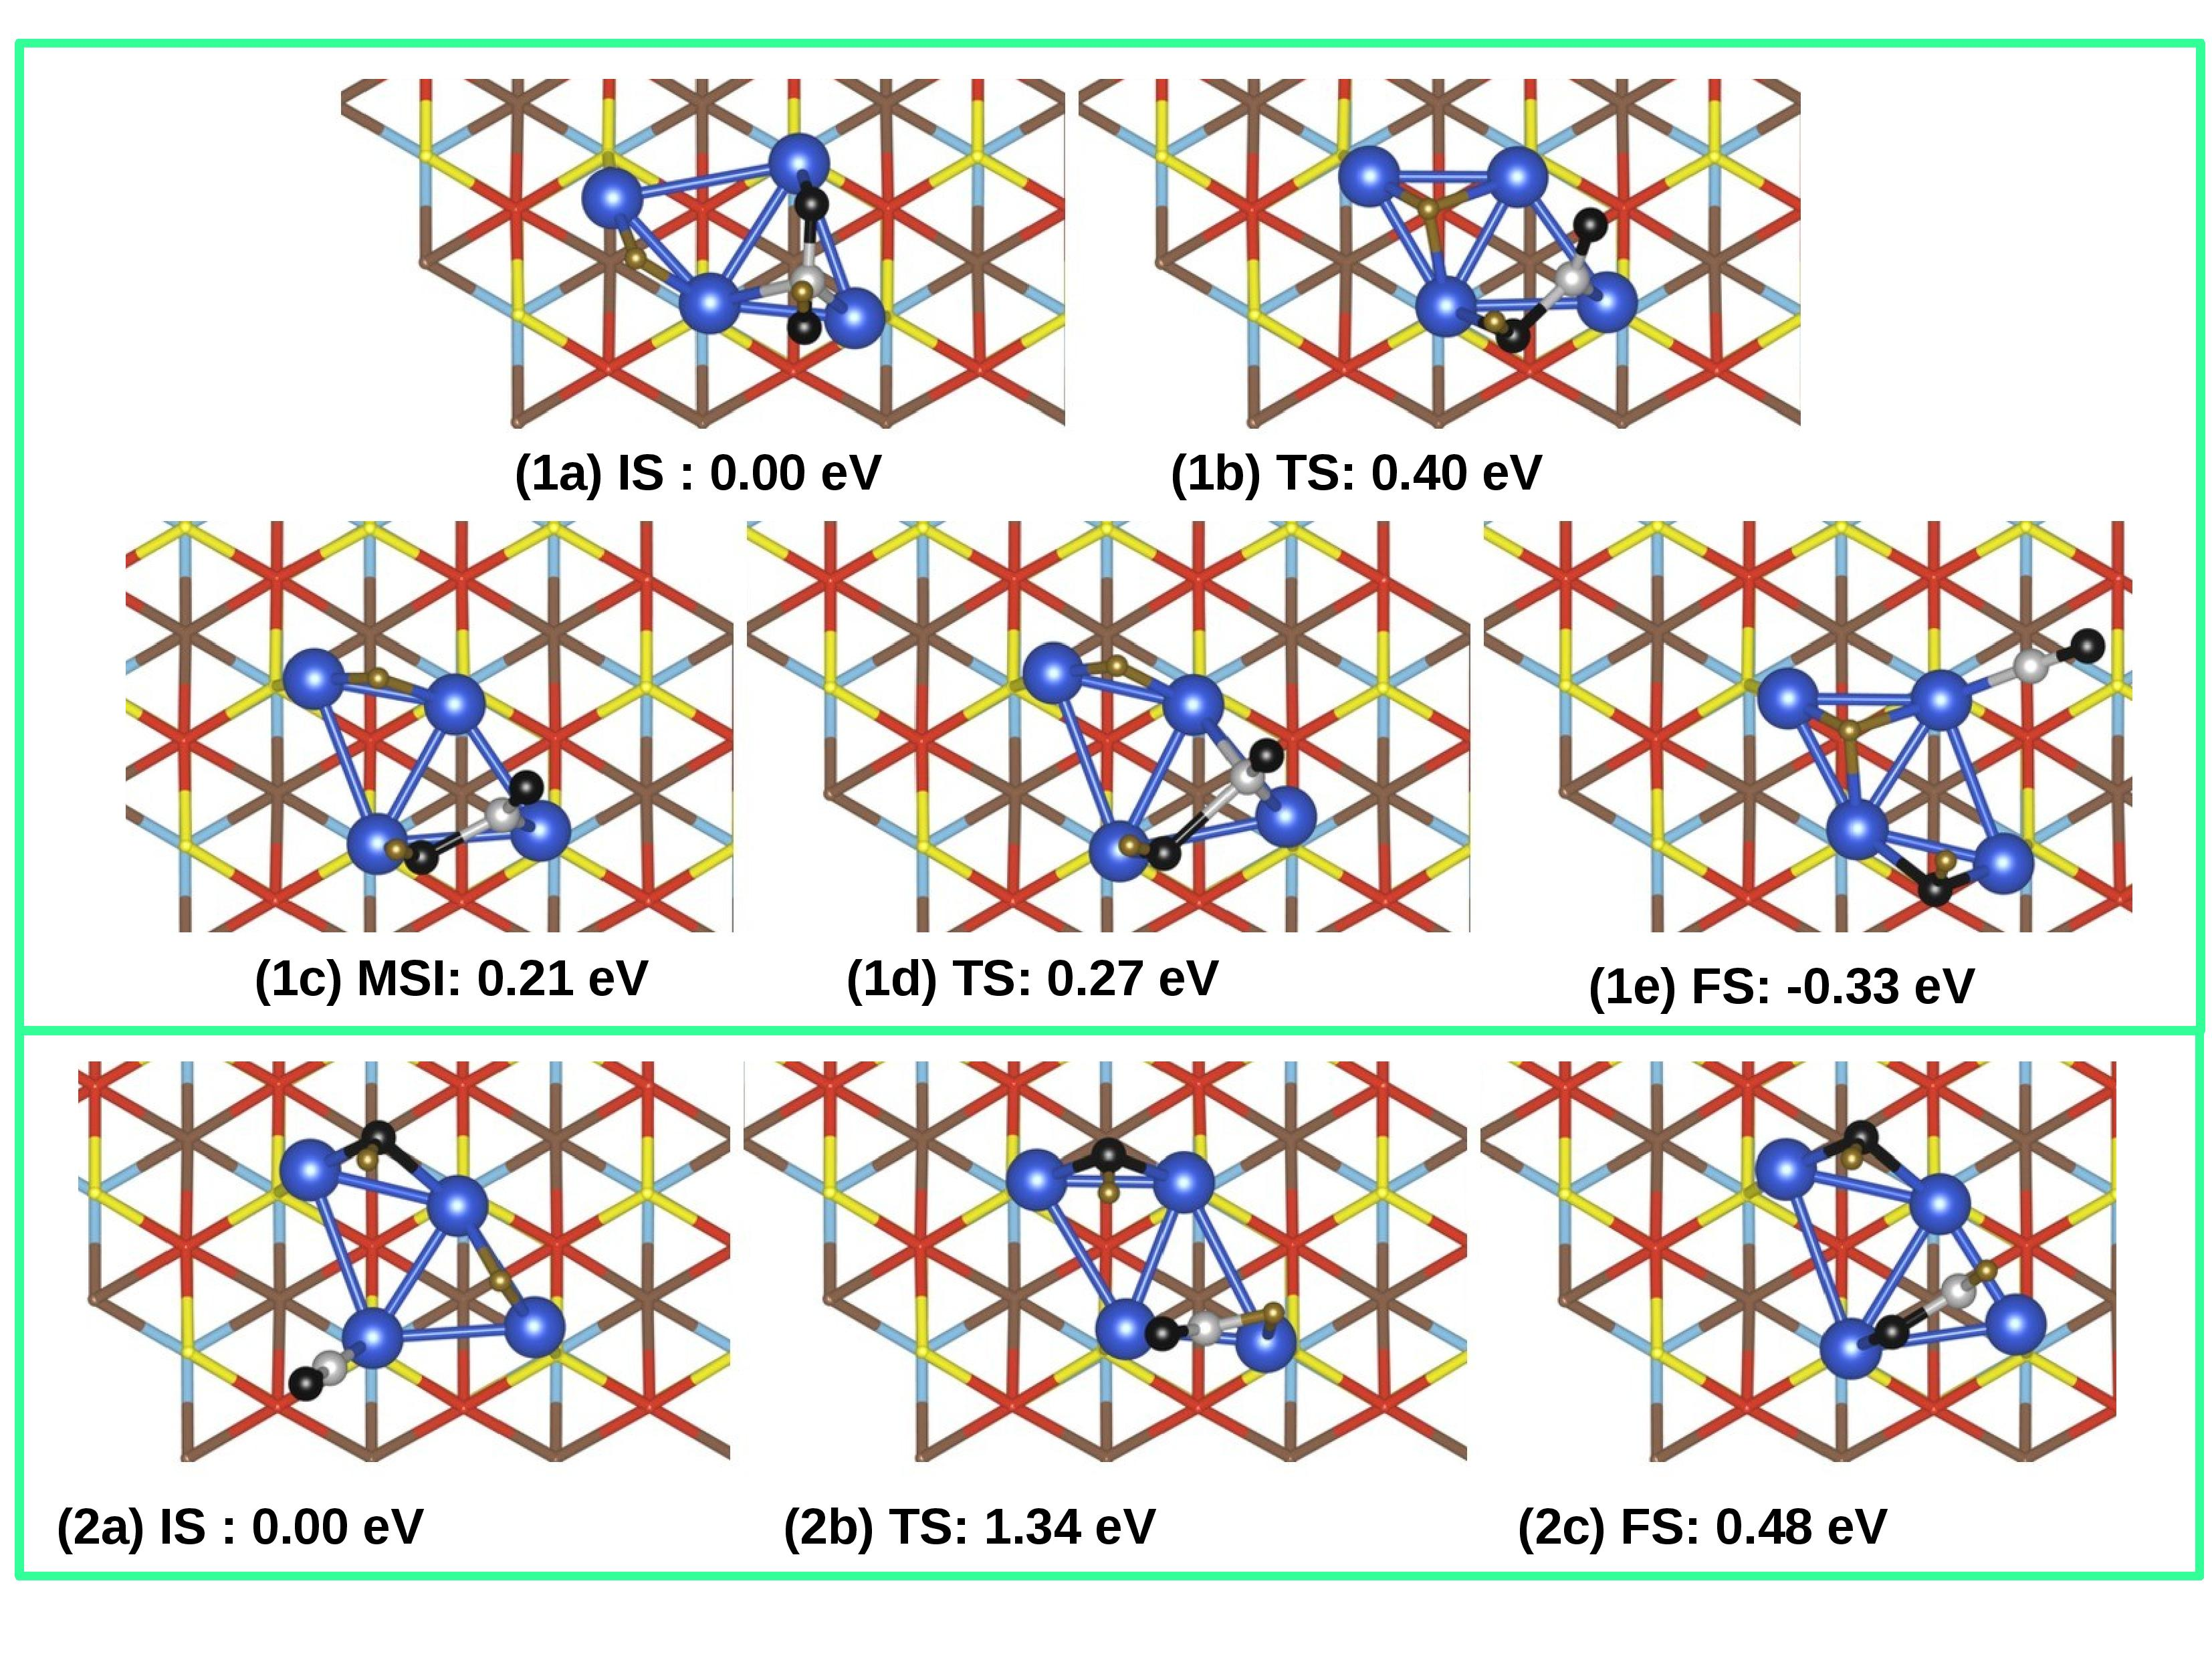
\includegraphics[width=0.9\textwidth]{./Appendix3/figures_si/p_109.jpg}
  \end{center}
    \caption{Reaction in top (rhombus tetramer, 1a-1e) and bottom (tetrahedron tetramer, 2a-2c) panel: *COOH + *H $\rightarrow$ *CO + *OH + *H.   }
  \label{fig:si-109}
\end{figure}

\begin{figure}
  \begin{center}
    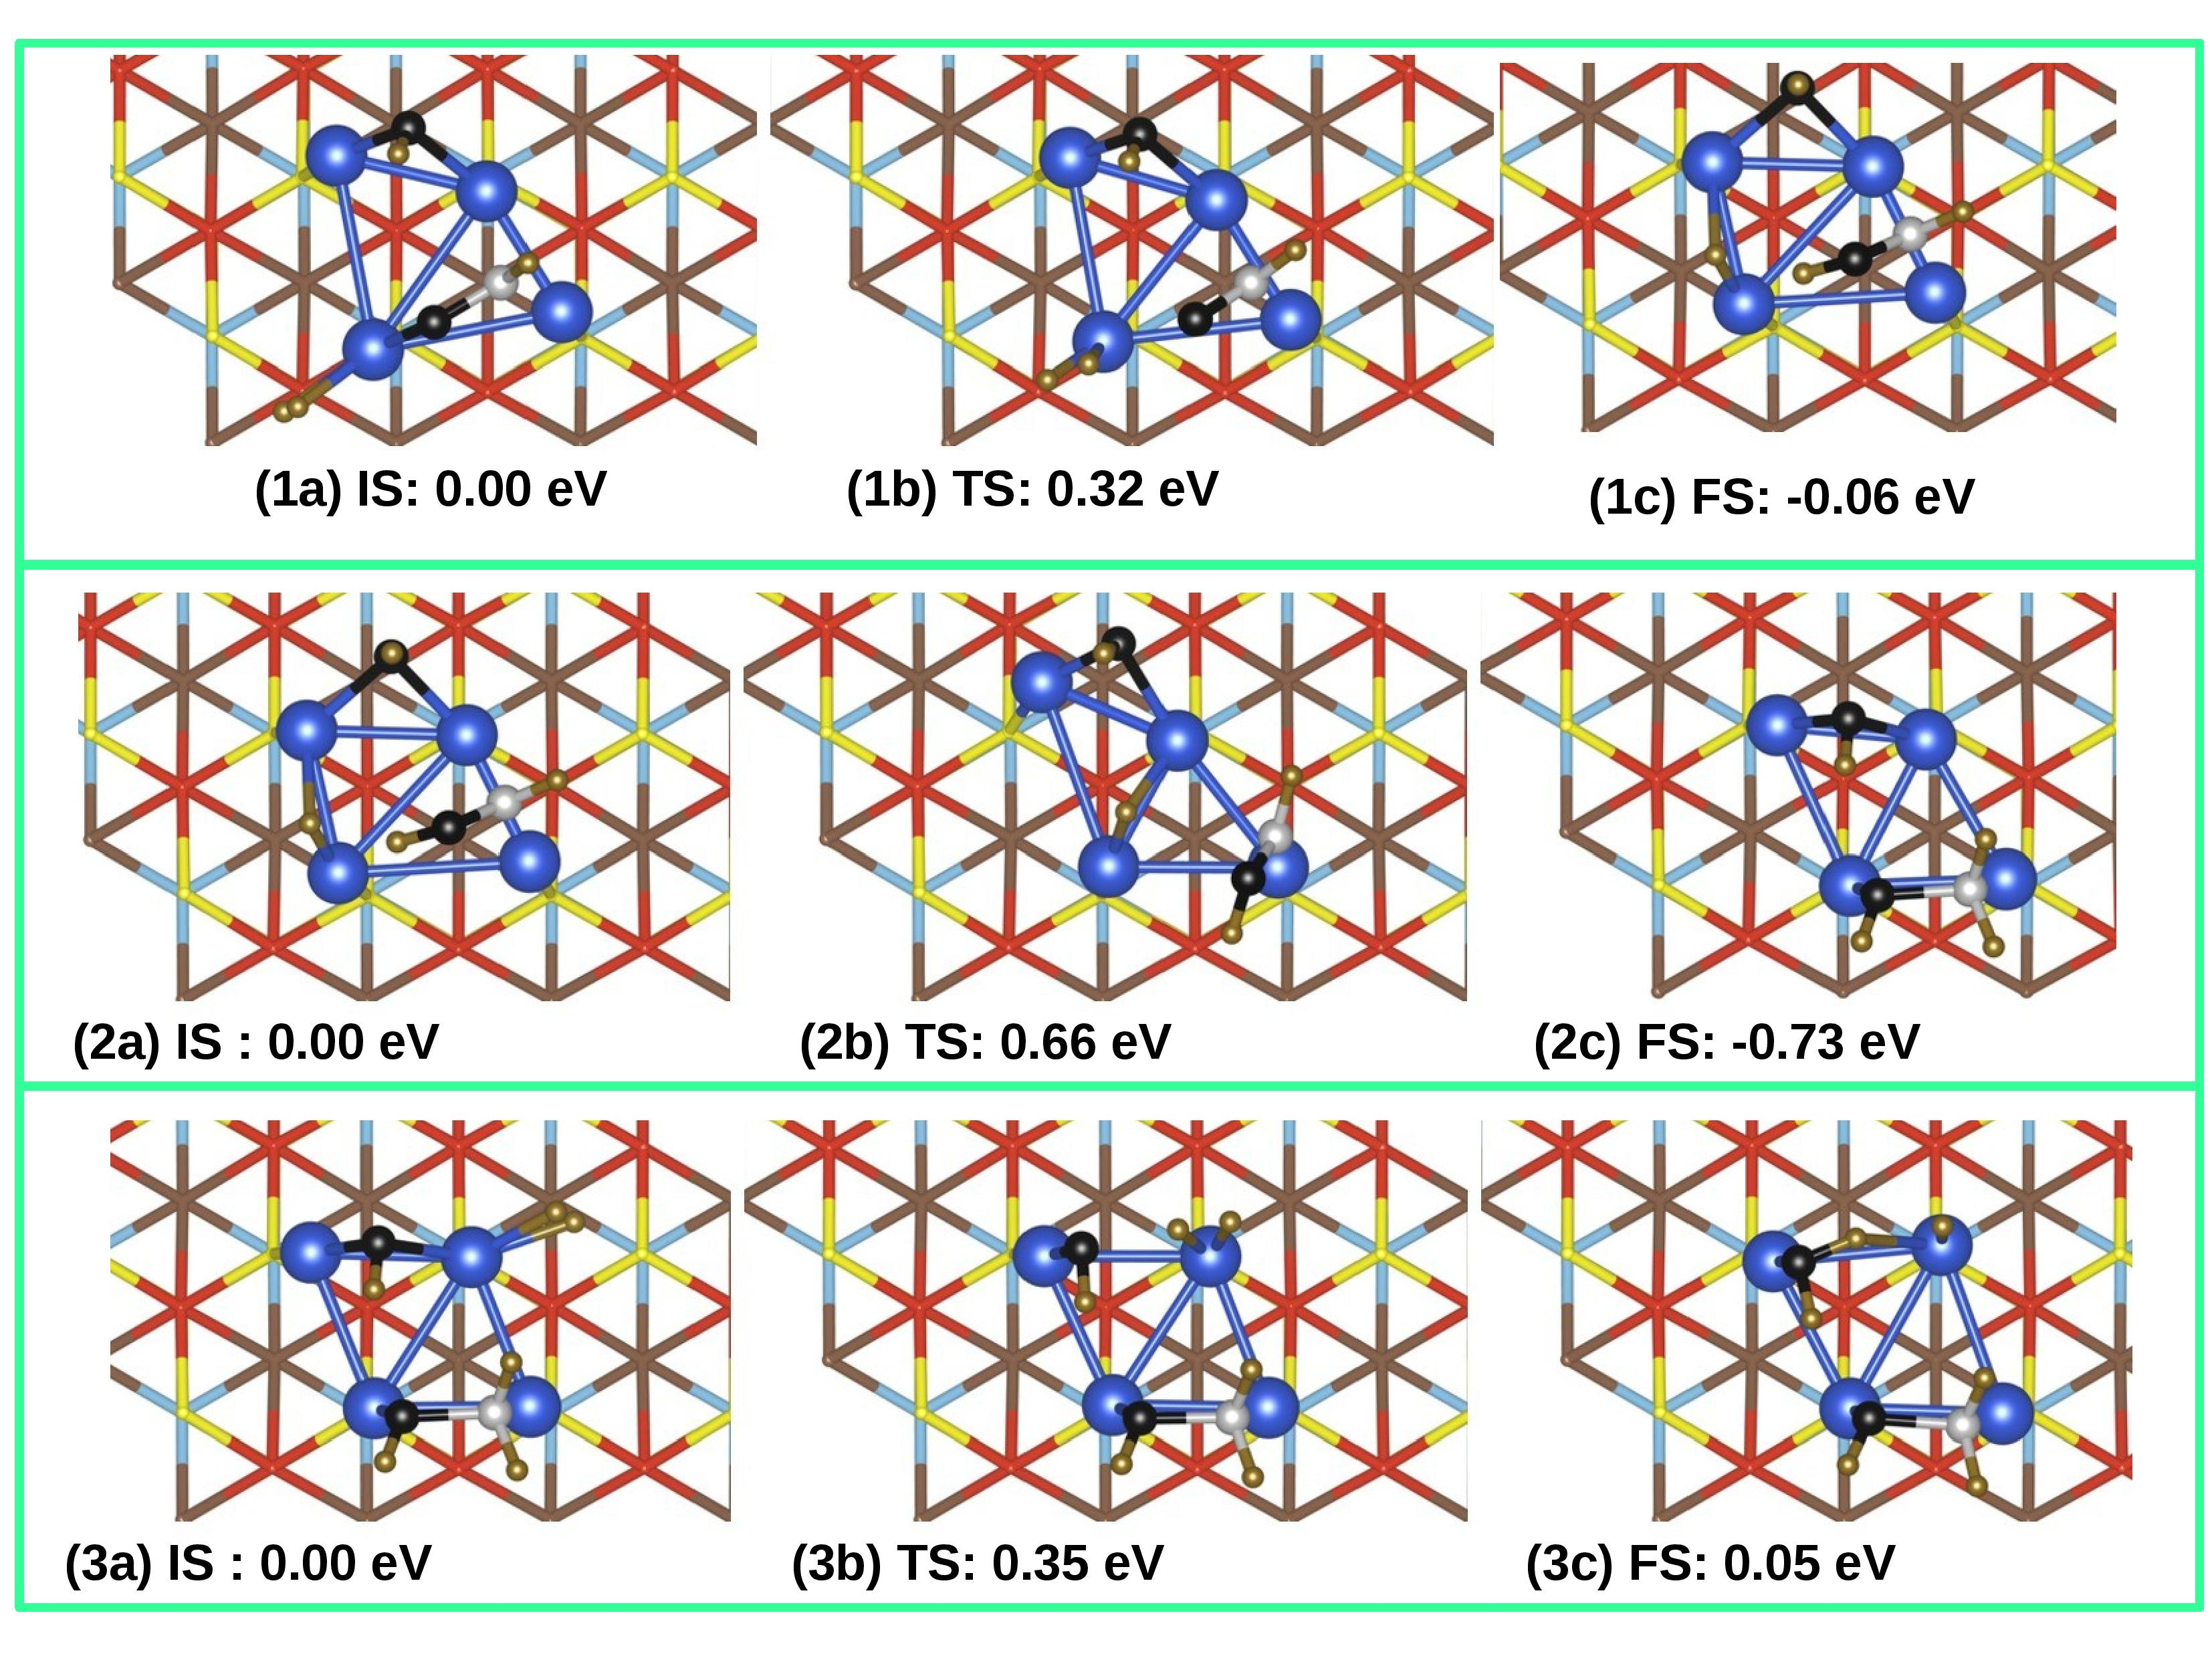
\includegraphics[width=0.9\textwidth]{./Appendix3/figures_si/p_110.jpg}
  \end{center}
    \caption{Reaction in top (rhombus tetramer, 1a-1c) panel: *HCO + *OH + *H$_2$ $\rightarrow$ *CHOH + *OH + *H. Reaction in middle (rhombus tetramer, 2a-2c) panel: : *CHOH  + *OH + *H $\rightarrow$ *CH$_2$OH + *OH. Reaction in bottom (rhombus tetramer, 3a-3c) panel: *CH$_2$OH  + *OH + *H$_2$ $\rightarrow$ *CH$_2$OH + *H$_2$O + *H. }
  \label{fig:si-110}
\end{figure}

\begin{figure}
  \begin{center}
    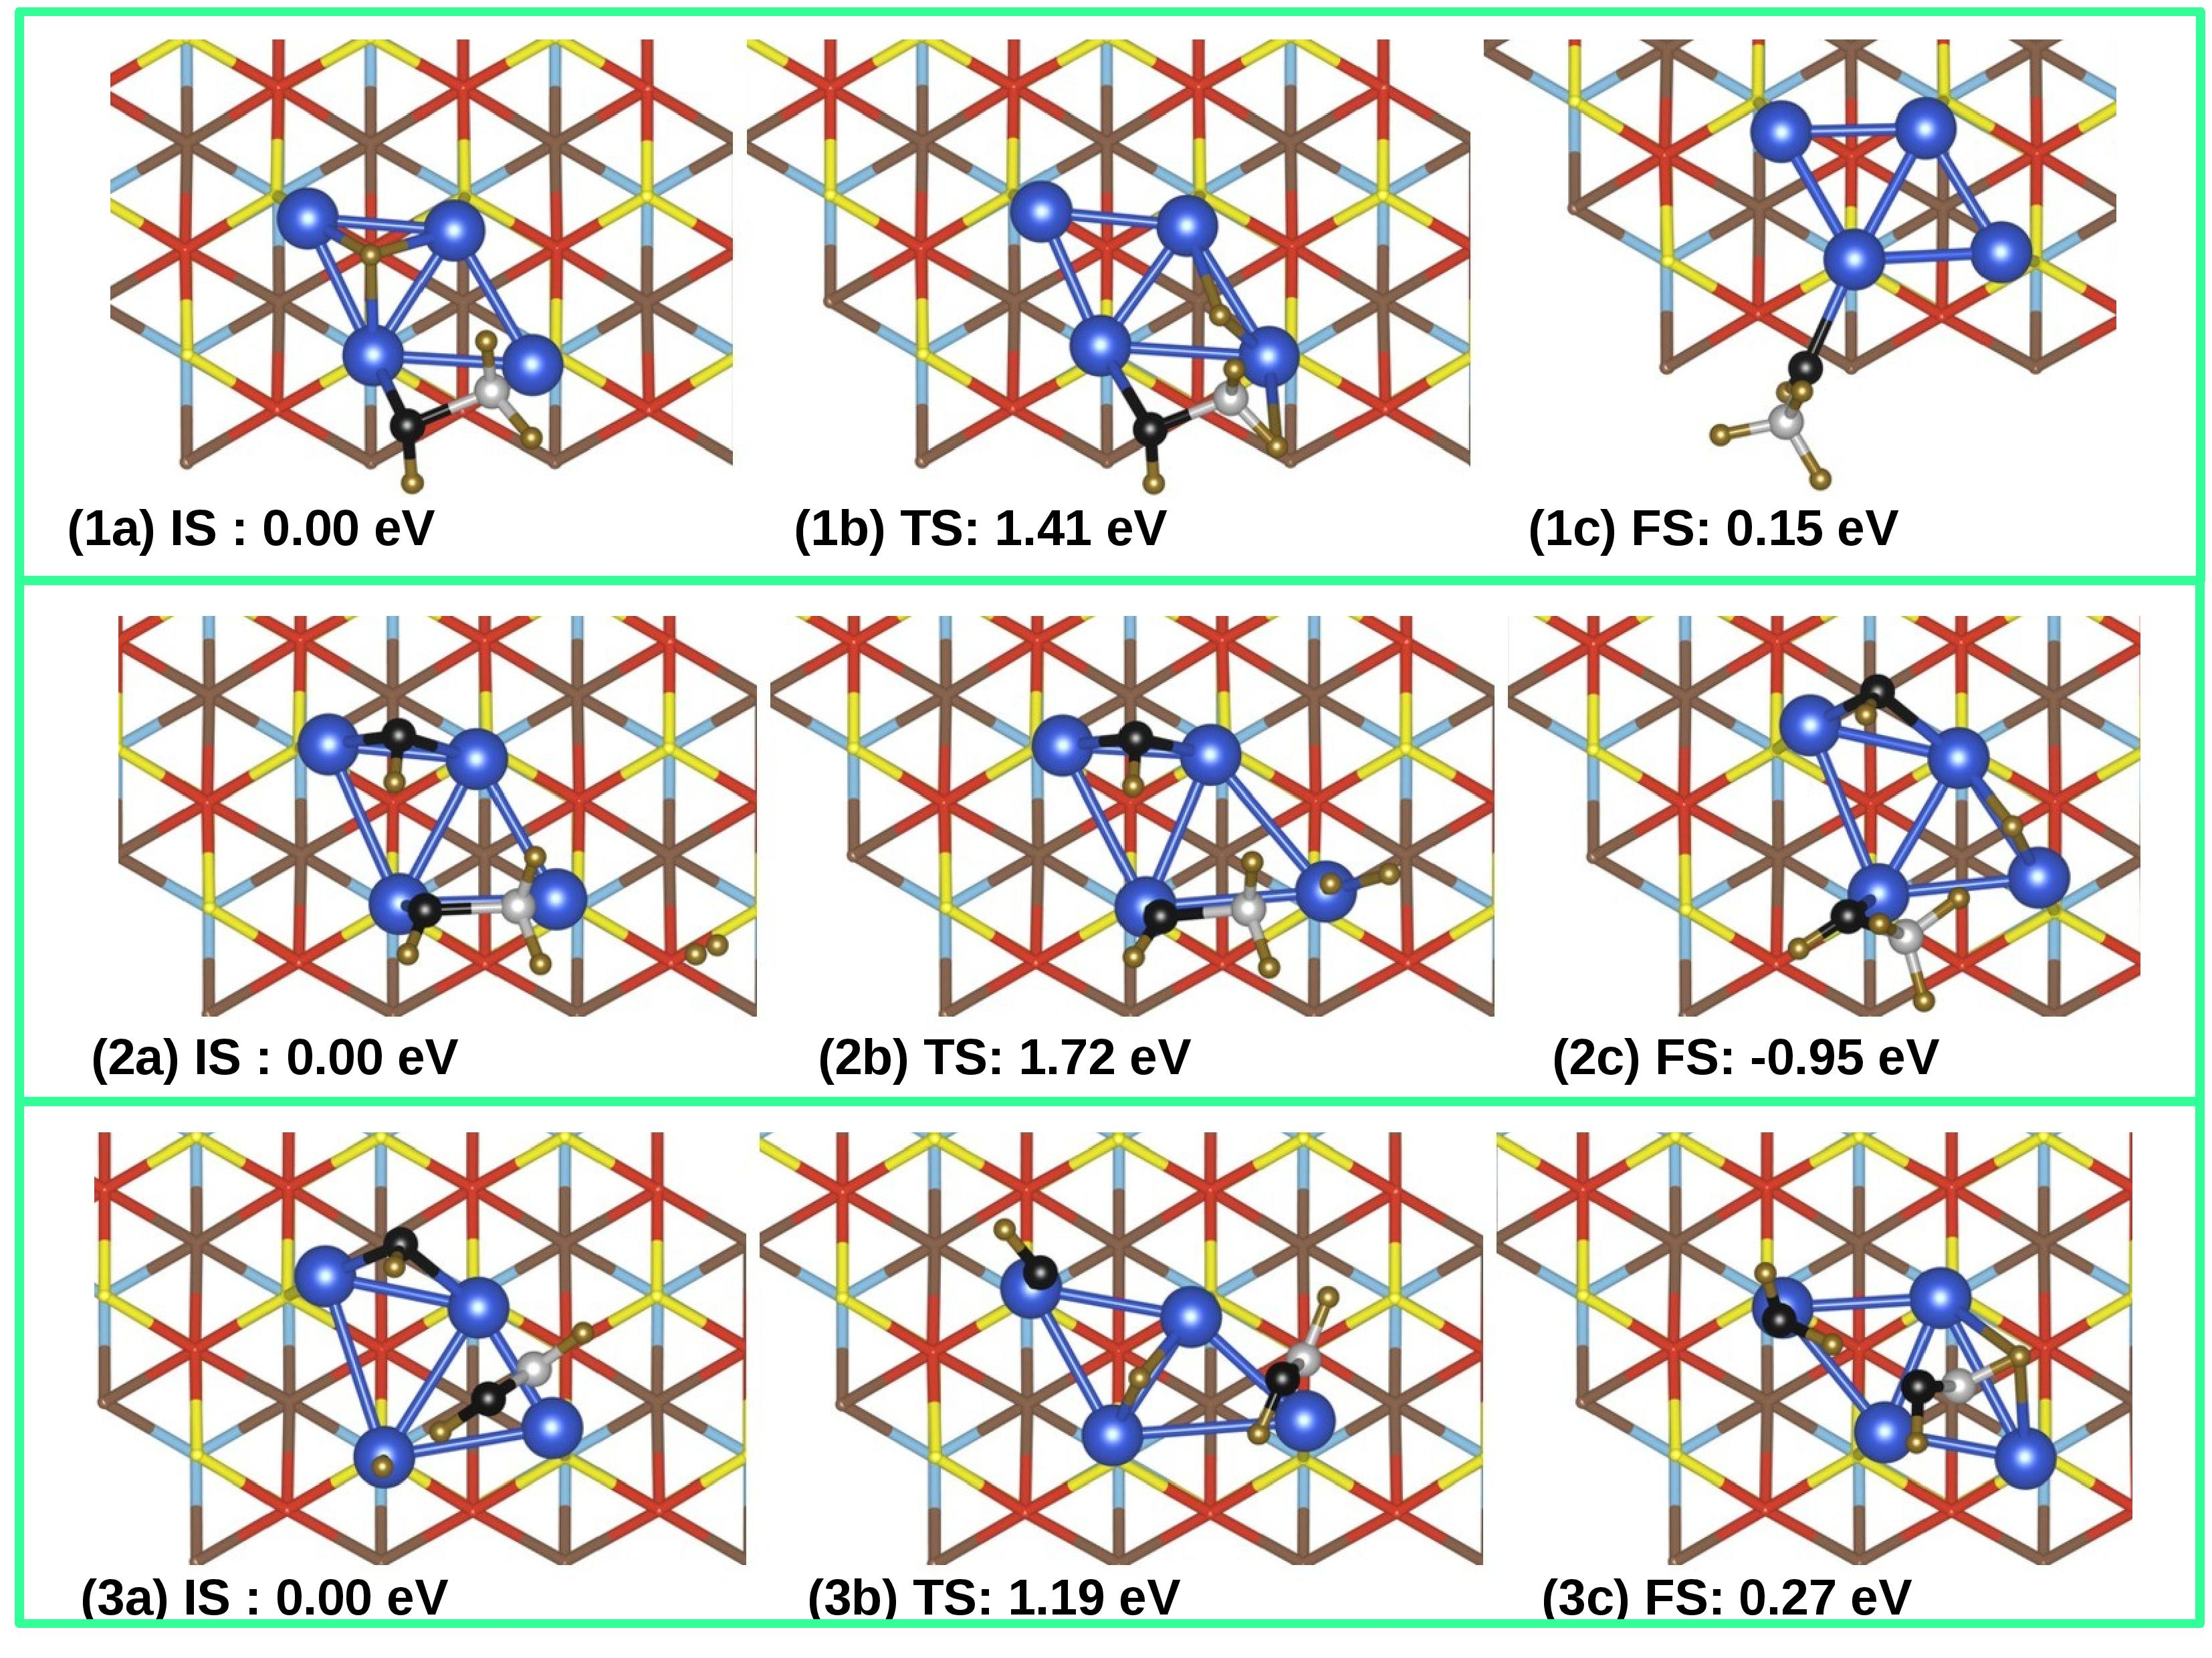
\includegraphics[width=0.9\textwidth]{./Appendix3/figures_si/p_111.jpg}
  \end{center}
    \caption{ Reaction in top (rhombus tetramer, 1a-1c) panel: *CH$_2$OH + *H $\rightarrow$ *CH$_3$OH. Reaction in middle (rhombus tetramer, 2a-2c) panel: *CH$_2$OH + *OH + *H$_2$ $\rightarrow$ *CH$_3$OH + *OH + *H. Reaction in bottom (rhombus tetramer, 3a-3c) panel: *CHOH + *OH + *H $\rightarrow$ *CHOH + *H$_2$O.   }
  \label{fig:si-111}
\end{figure}

\begin{figure}
  \begin{center}
    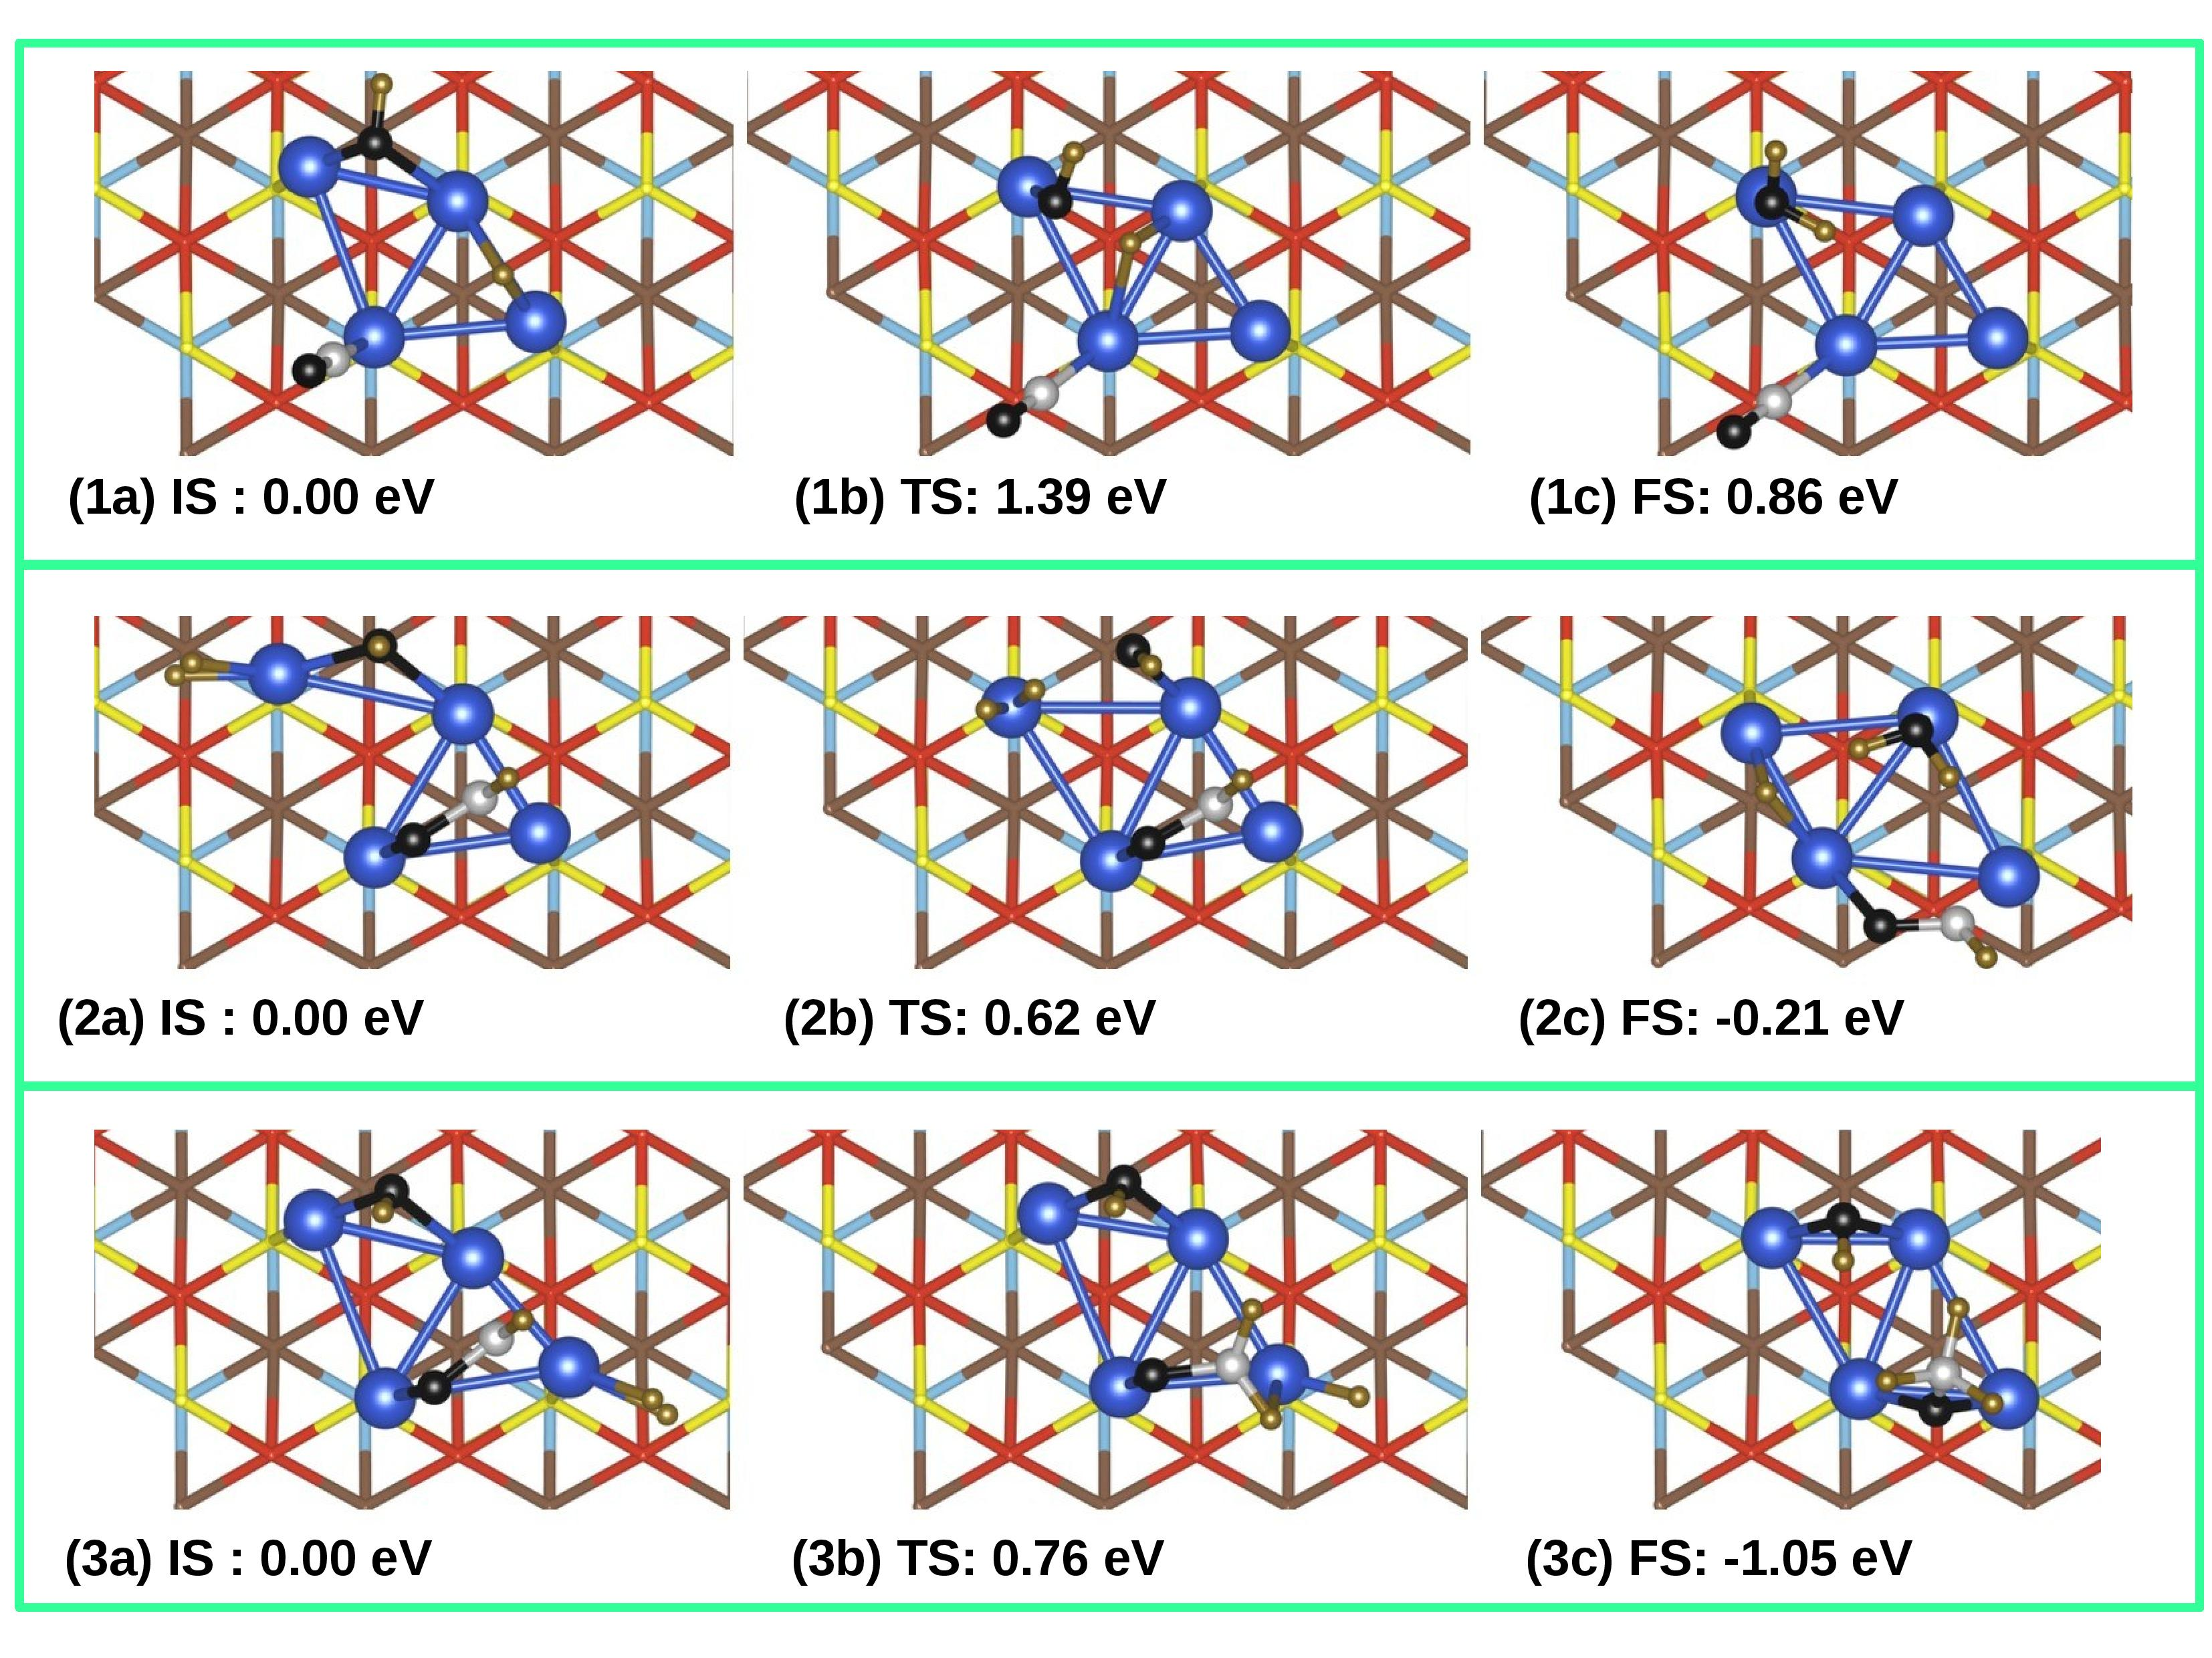
\includegraphics[width=0.9\textwidth]{./Appendix3/figures_si/p_112.jpg}
  \end{center}
    \caption{ Reaction in top (rhombus tetramer, 1a-1c) panel: *CO + *OH + *H $\rightarrow$ *CO + *H$_2$O. Reaction in middle (rhombus tetramer, 2a-2c) panel: *HCO + *OH + *H$_2$ $\rightarrow$ *HCO + *H$_2$O + *H. Reaction in bottom (rhombus tetramer, 3a-3c) panel: *HCO + *OH + *H$_2$ $\rightarrow$ *CH$_3$O + *OH.  }
  \label{fig:si-112}
\end{figure}

\begin{figure}
  \begin{center}
    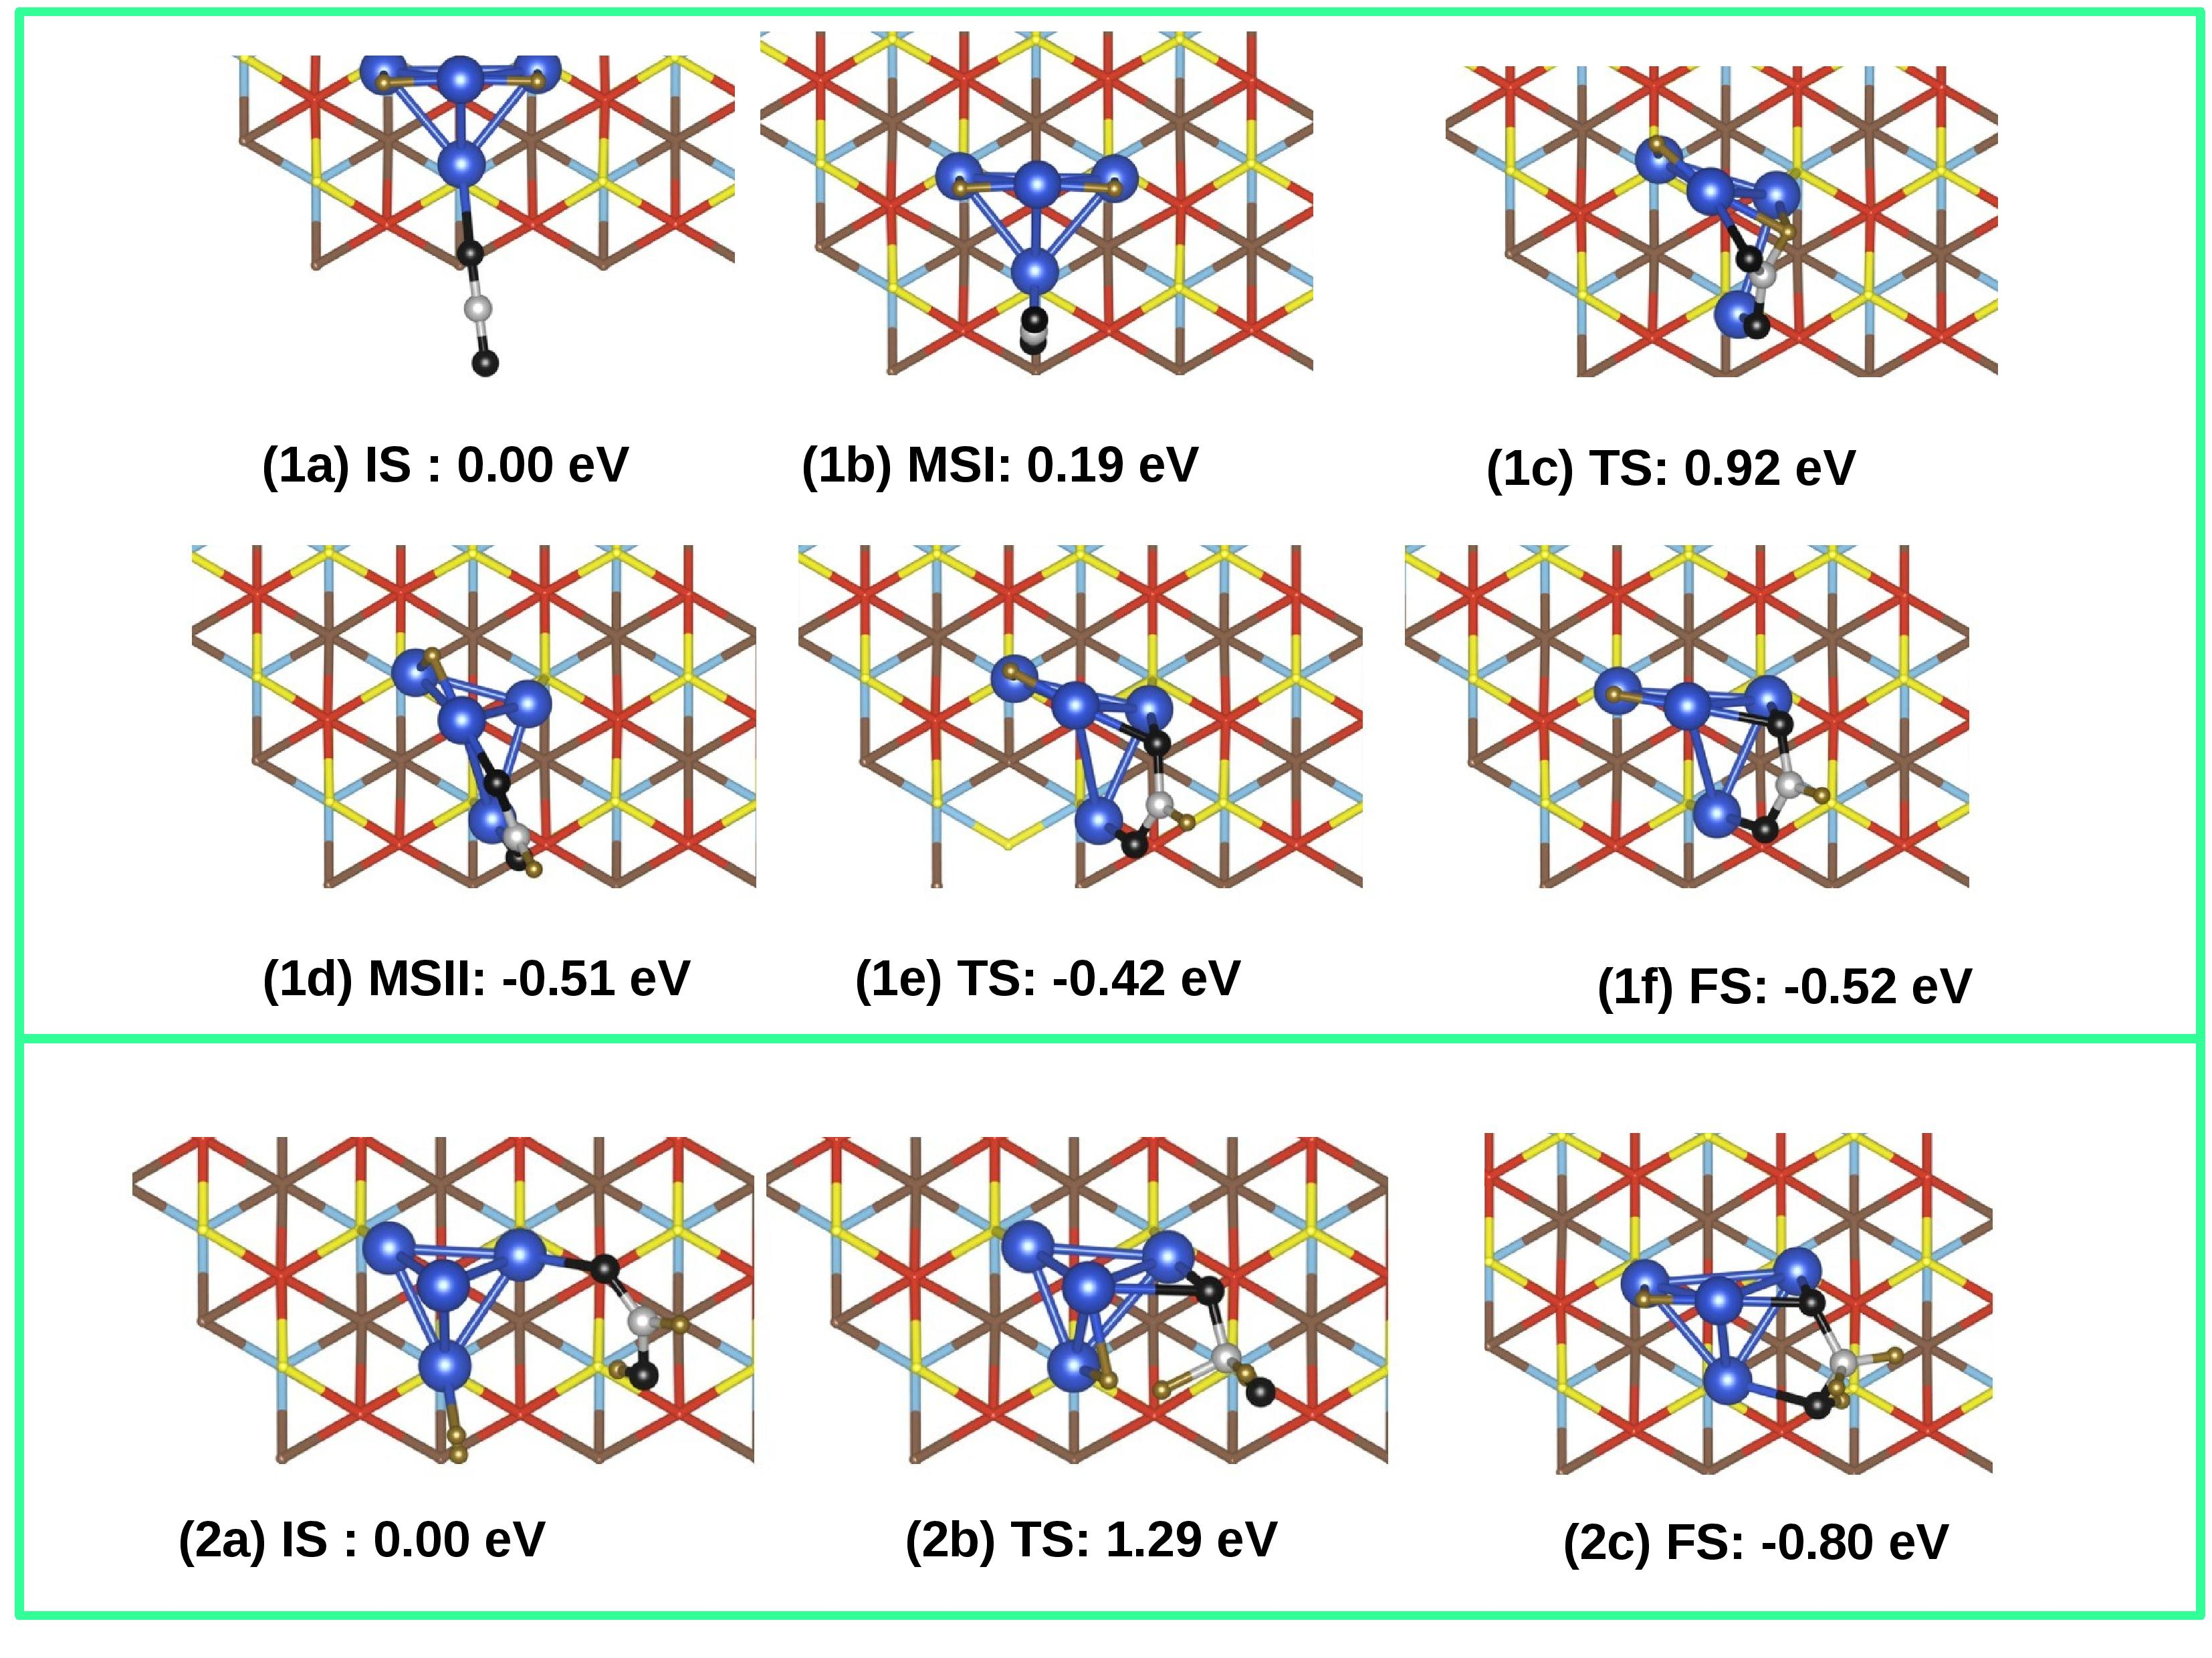
\includegraphics[width=0.9\textwidth]{./Appendix3/figures_si/p_113.jpg}
  \end{center}
    \caption{ Reaction in top (tetrahedron tetramer, 1a-1f) panel: *CO$_2$ + *H + *H $\rightarrow$ *HCOO + *H. Reaction in bottom (tetrahedron tetramer, 2a-2c) panel: *HCOOH + *H$_2$ $\rightarrow$ *CH$_2$OOH + *H.  }
  \label{fig:si-113}
\end{figure}

\begin{figure}
  \begin{center}
    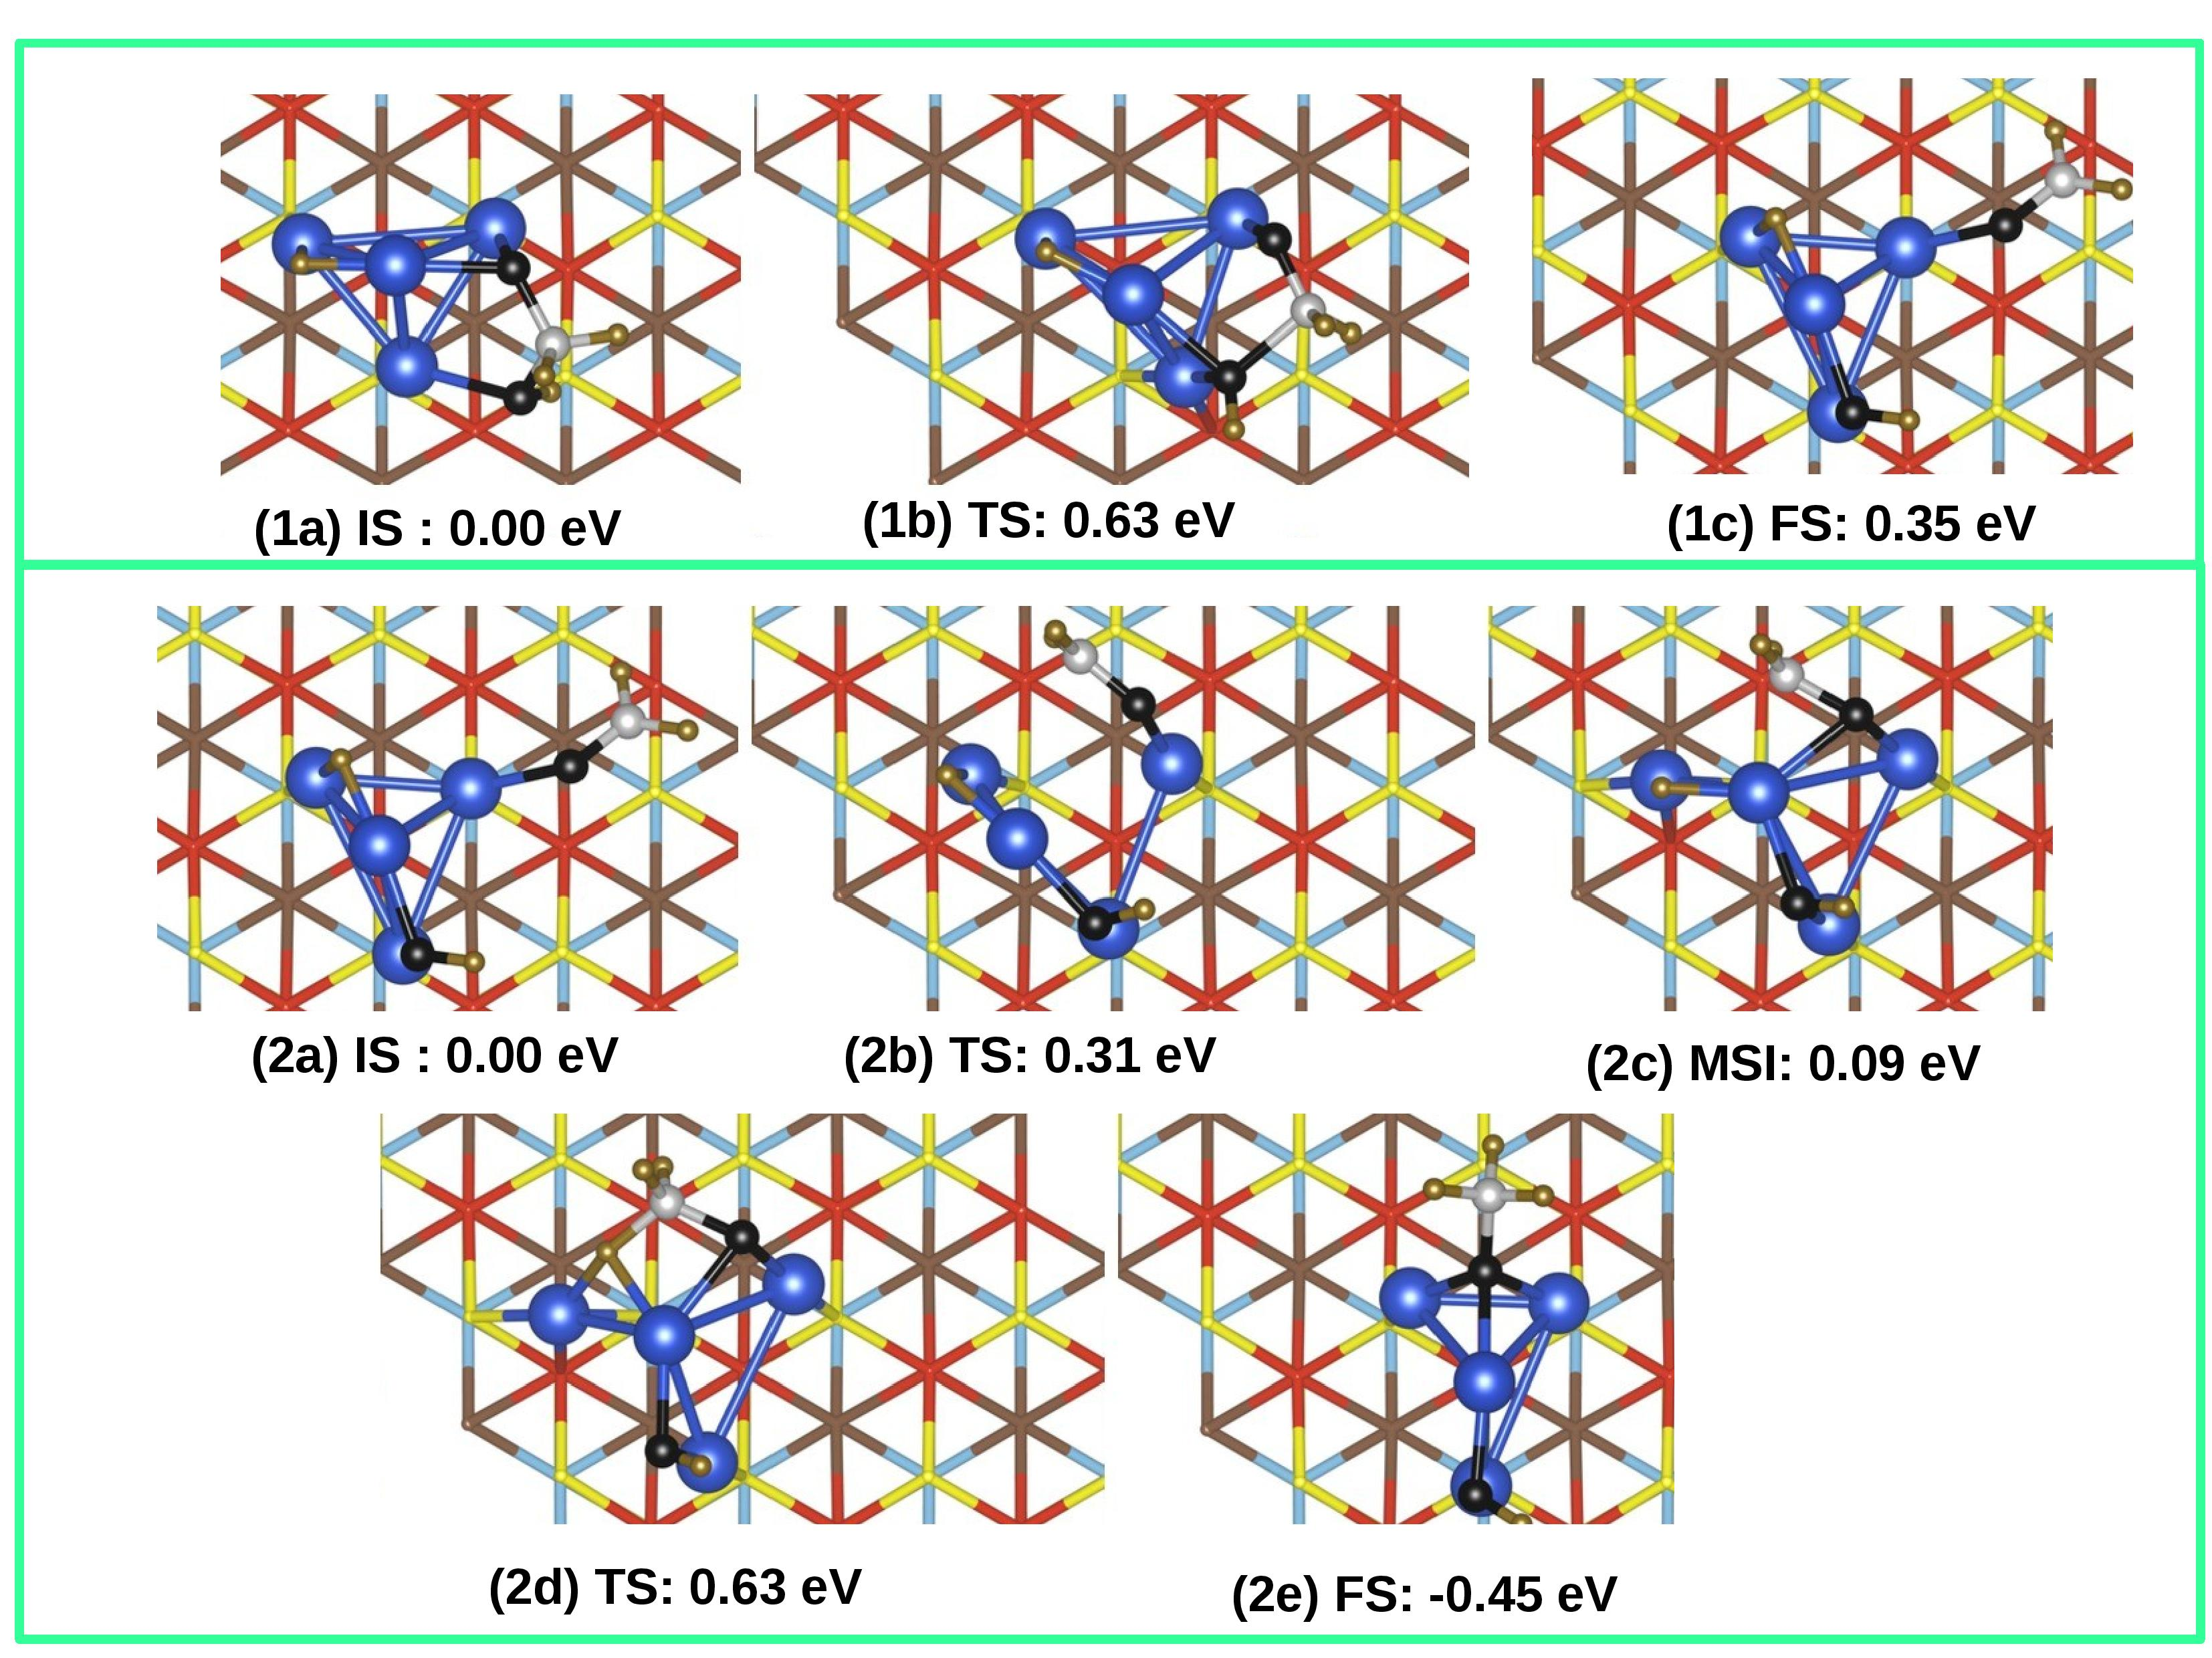
\includegraphics[width=0.9\textwidth]{./Appendix3/figures_si/p_114.jpg}
  \end{center}
    \caption{ Reaction in top (tetrahedron tetramer, 1a-1c) panel: *CH$_2$OOH + *H $\rightarrow$ *CH$_2$O + *OH + *H. Reaction in bottom (tetrahedron tetramer, 2a-2e) panel: *CH$_2$O + *OH + *H $\rightarrow$ *CH$_3$O + *OH. }
  \label{fig:si-114}
\end{figure}

\begin{figure}
  \begin{center}
    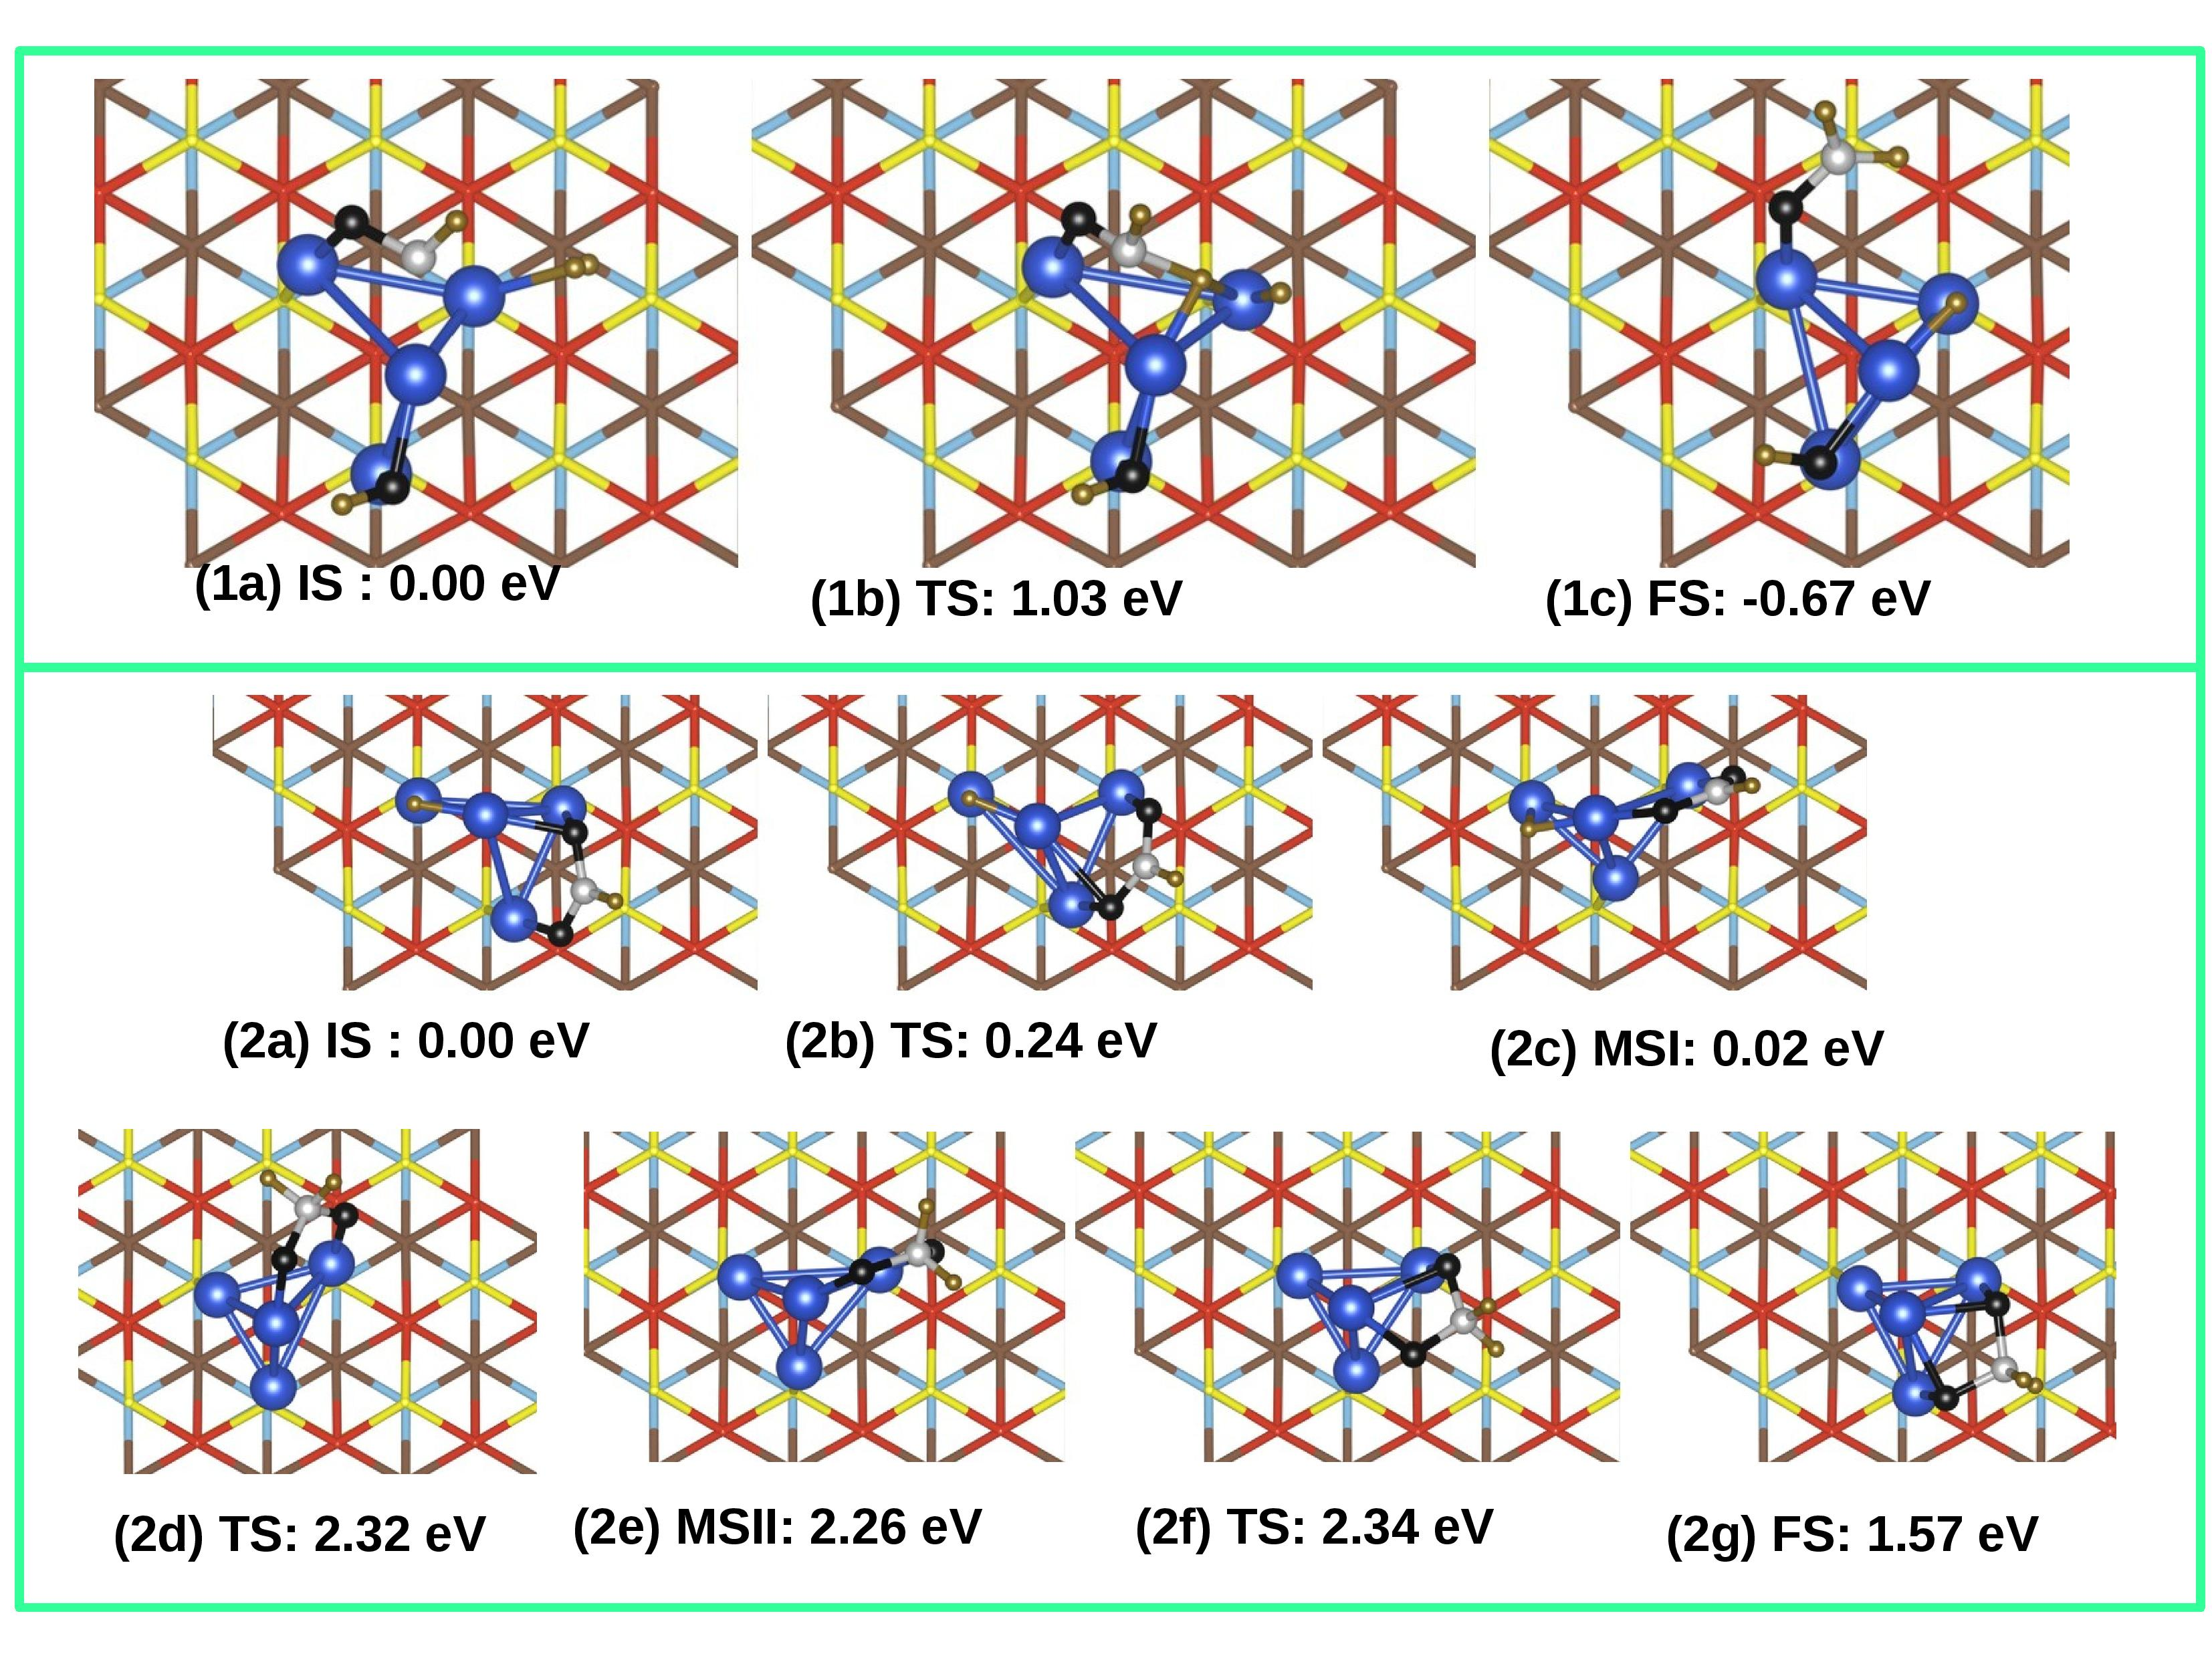
\includegraphics[width=0.9\textwidth]{./Appendix3/figures_si/p_116.jpg}
  \end{center}
    \caption{Reaction in top (tetrahedron tetramer, 1a-1c) panel: *HCO + *OH + *H$_2$ $\rightarrow$ *CH$_2$O + *OH + *H. Reaction in bottom (tetrahedron tetramer, 2a-2g) panel: *HCOO + *H $\rightarrow$ *CH$_2$OO.  }
  \label{fig:si-115}
\end{figure}

\begin{figure}
  \begin{center}
    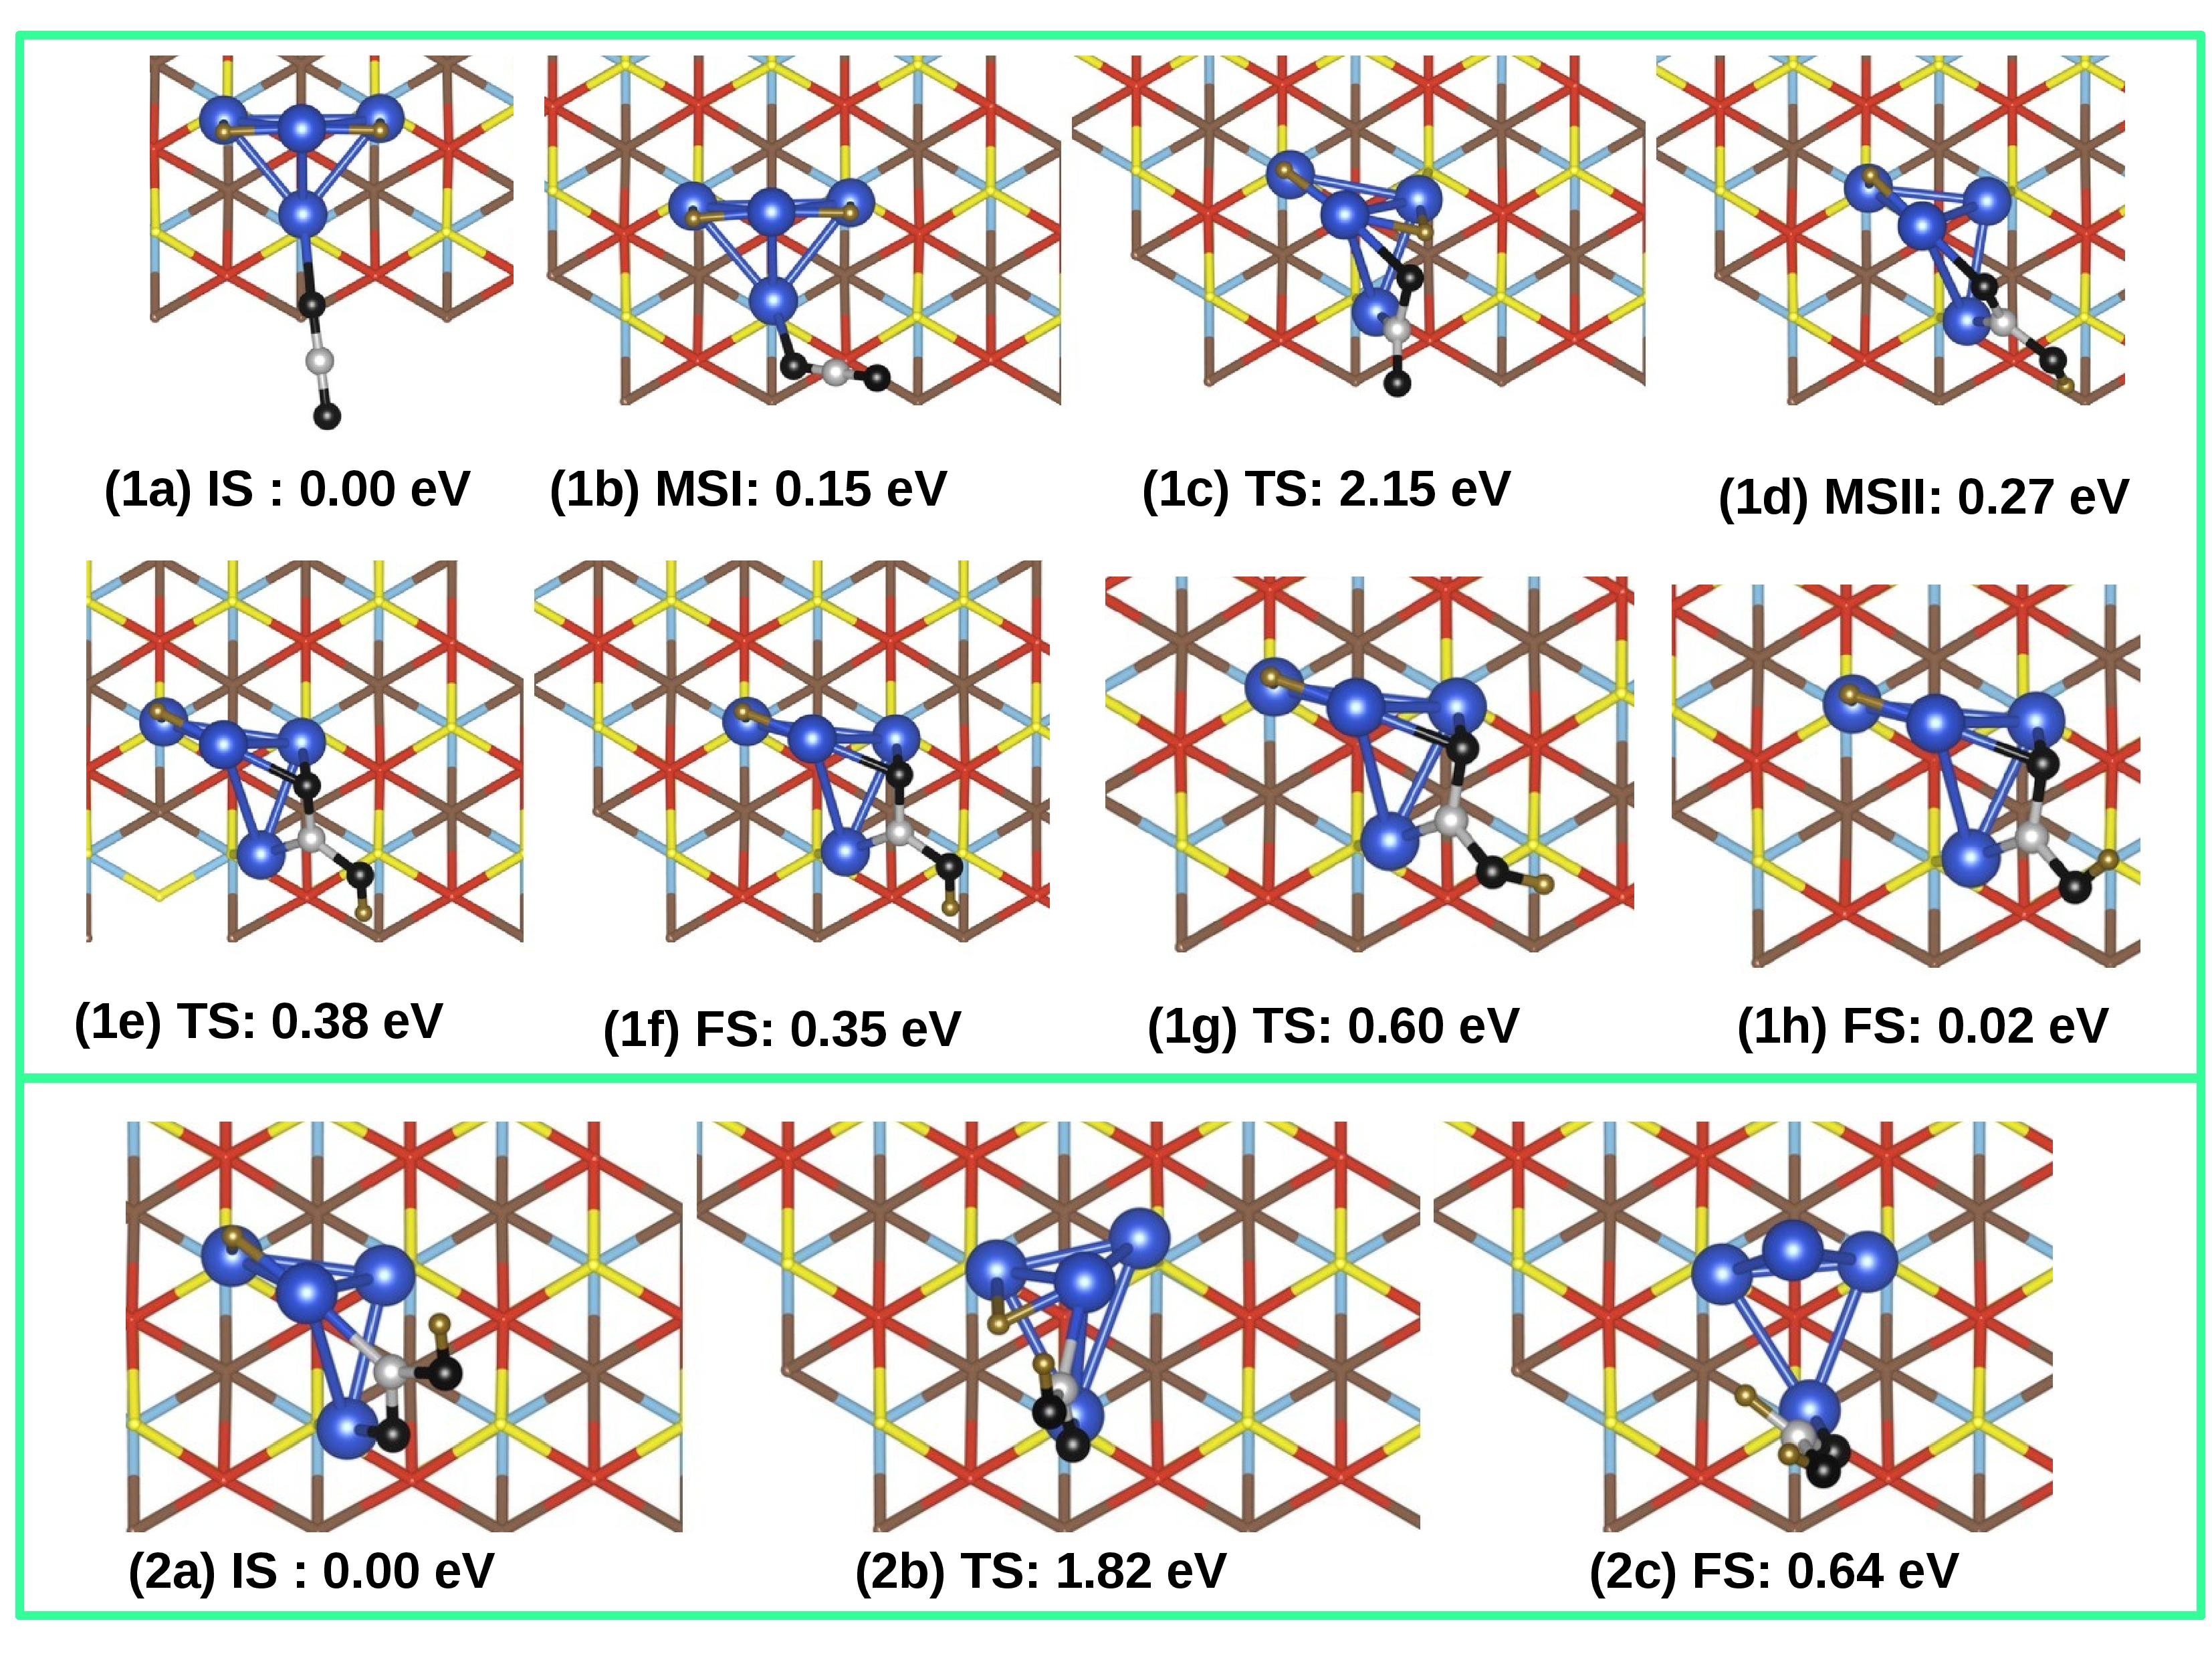
\includegraphics[width=0.9\textwidth]{./Appendix3/figures_si/p_117.jpg}
  \end{center}
    \caption{Reaction in top (tetrahedron tetramer, 1a-1h) panel: *CO$_2$ + *H  + *H $\rightarrow$ *COOH + *H. Reaction in bottom (tetrahedron tetramer, 2a-2c) panel: *COOH + *H $\rightarrow$ *HCOOH.  }
  \label{fig:si-116}
\end{figure}

\begin{figure}
  \begin{center}
    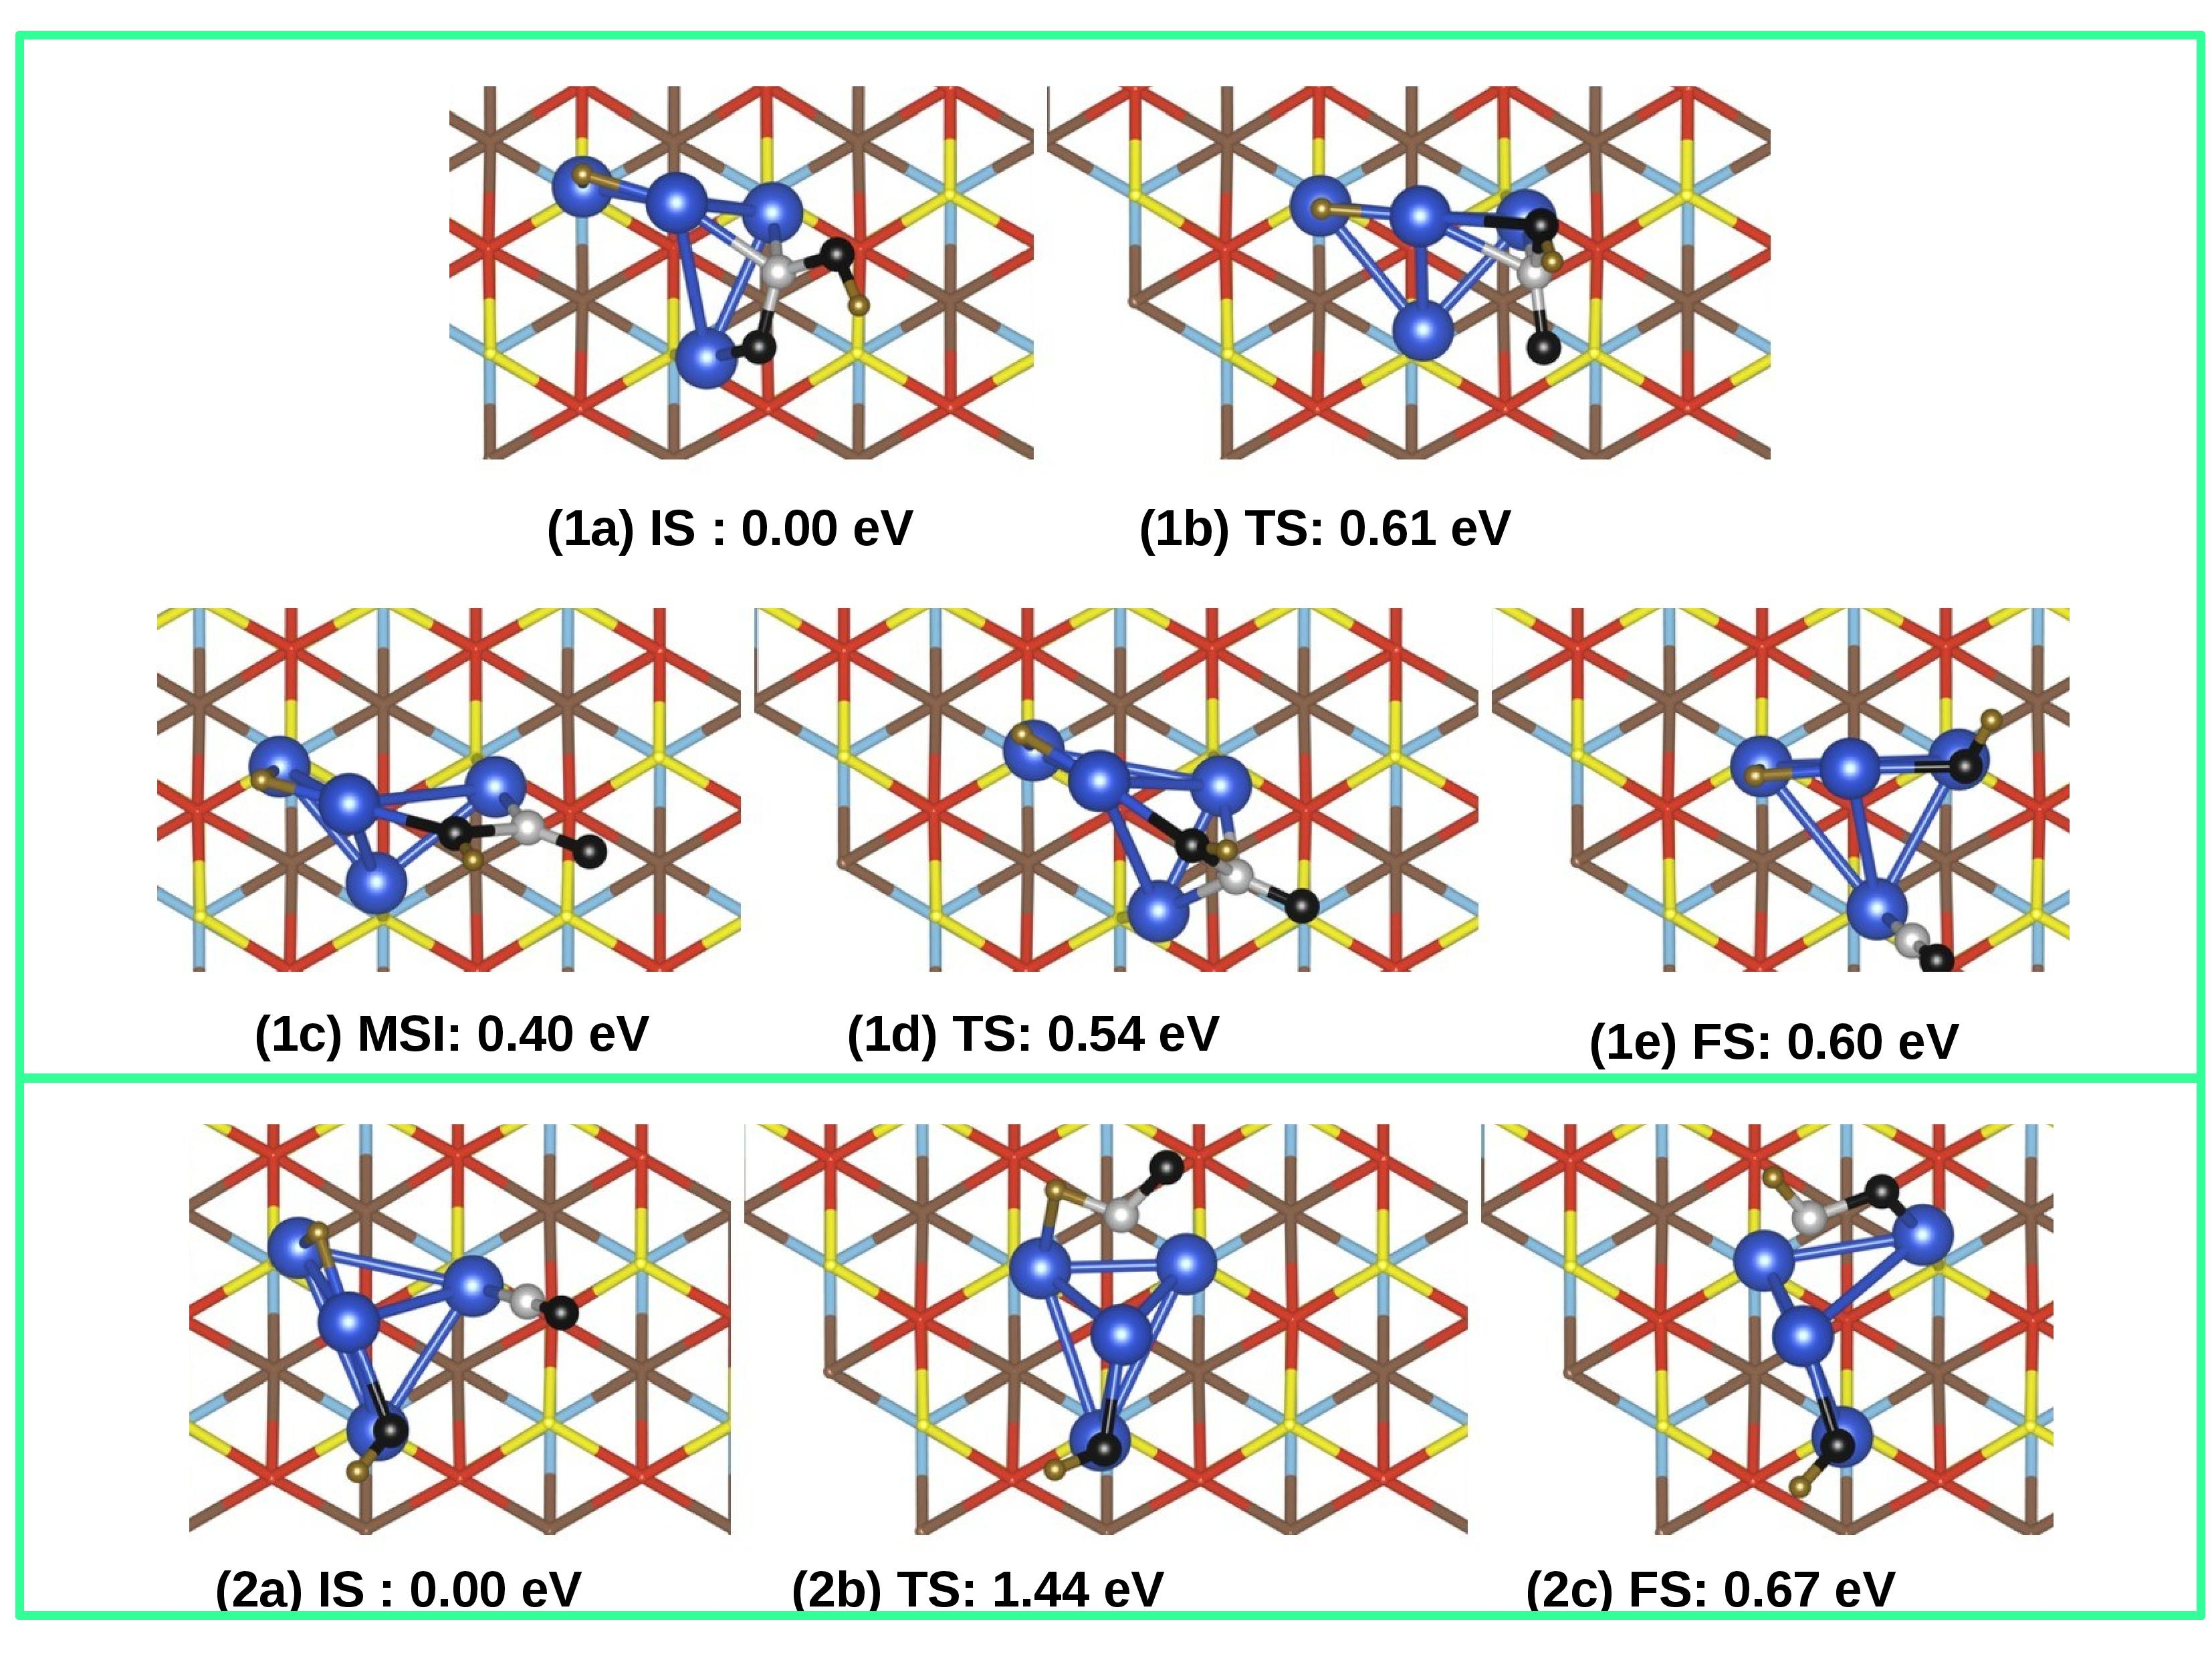
\includegraphics[width=0.9\textwidth]{./Appendix3/figures_si/p_118.jpg}
  \end{center}
    \caption{Reaction in top (tetrahedron tetramer, 1a-1e) panel: *COOH + *H $\rightarrow$ *CO + *OH + *H. Reaction in bottom (tetrahedron tetramer, 2a-2c) panel: *CO + *OH + *H $\rightarrow$ *HCO + *OH. }
  \label{fig:si-117}
\end{figure}

\begin{figure}
  \begin{center}
    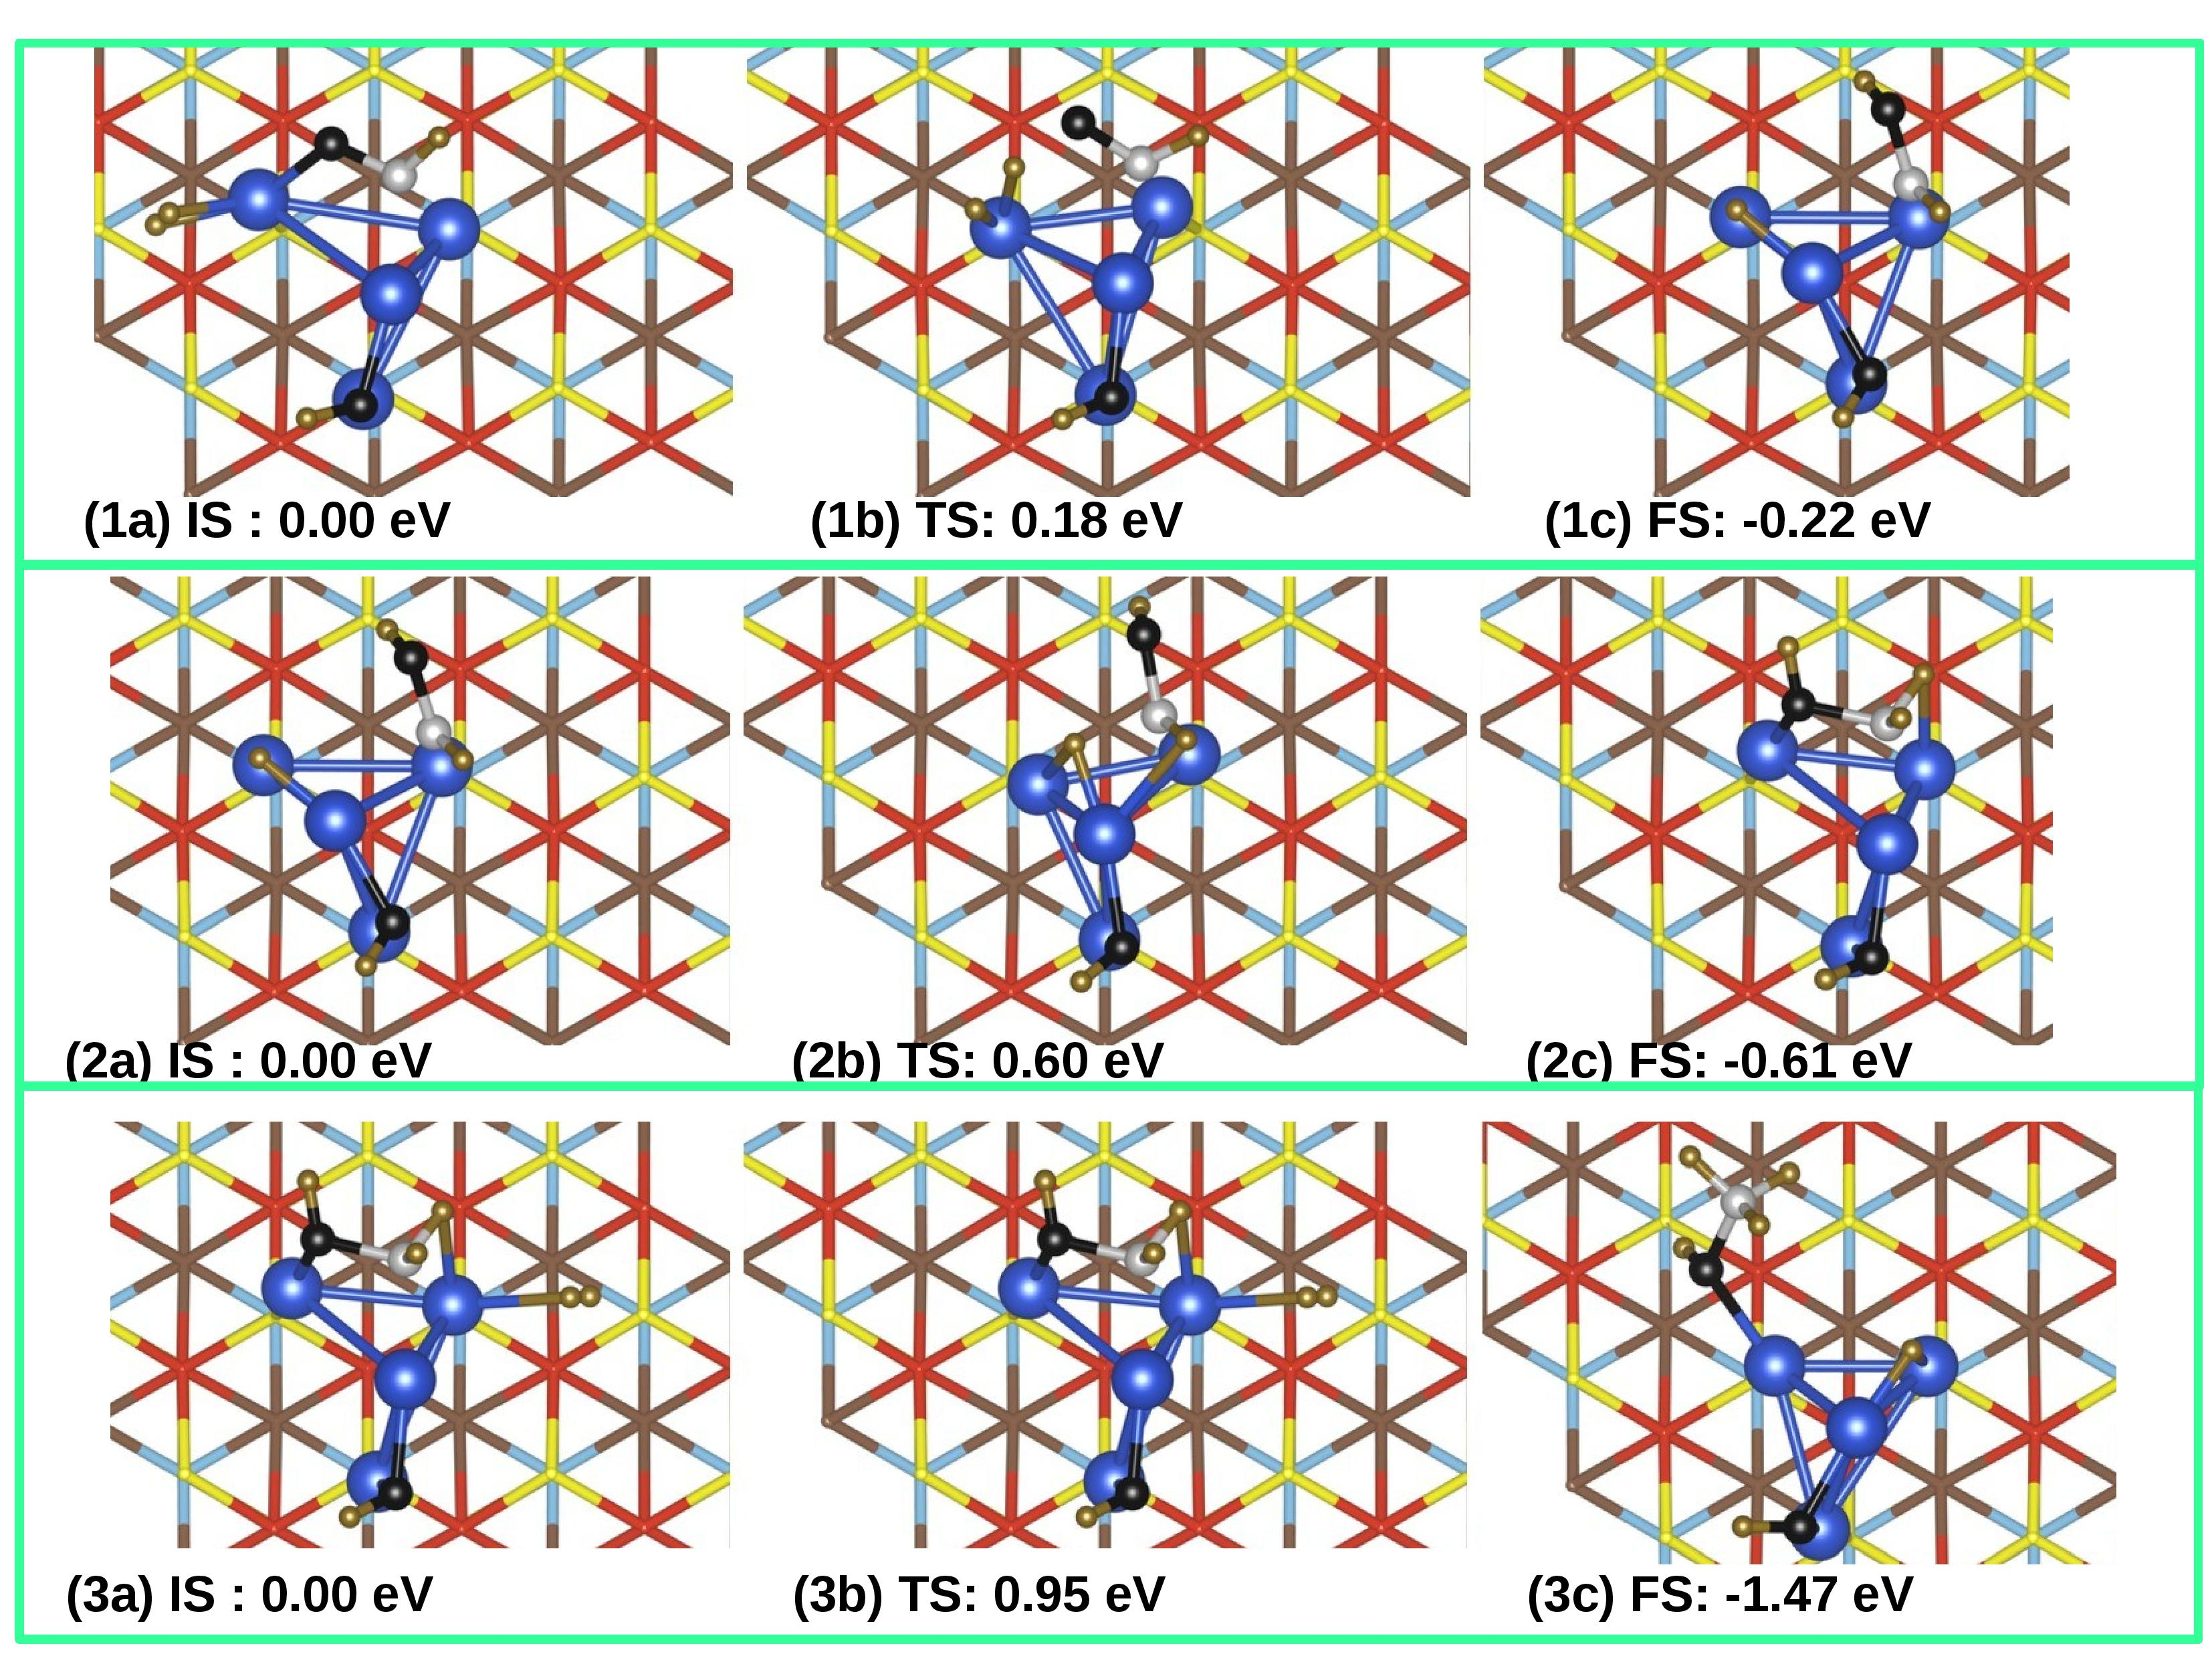
\includegraphics[width=0.9\textwidth]{./Appendix3/figures_si/p_119.jpg}
  \end{center}
    \caption{Reaction in top (tetrahedron tetramer, 1a-1c) panel: *HCO + *OH + *H$_2$ $\rightarrow$ *HCOH + *OH + *H. Reaction in middle (tetrahedron tetramer, 2a-2c) panel: *HCOH + *OH + *H $\rightarrow$ *CH$_2$OH + *OH. Reaction in bottom (tetrahedron tetramer, 3a-3c) panel: *CH$_2$OH + *OH + *H$_2$ $\rightarrow$ *CH$_3$OH + *OH + *H.  }
  \label{fig:si-118}
\end{figure}

\begin{figure}
  \begin{center}
    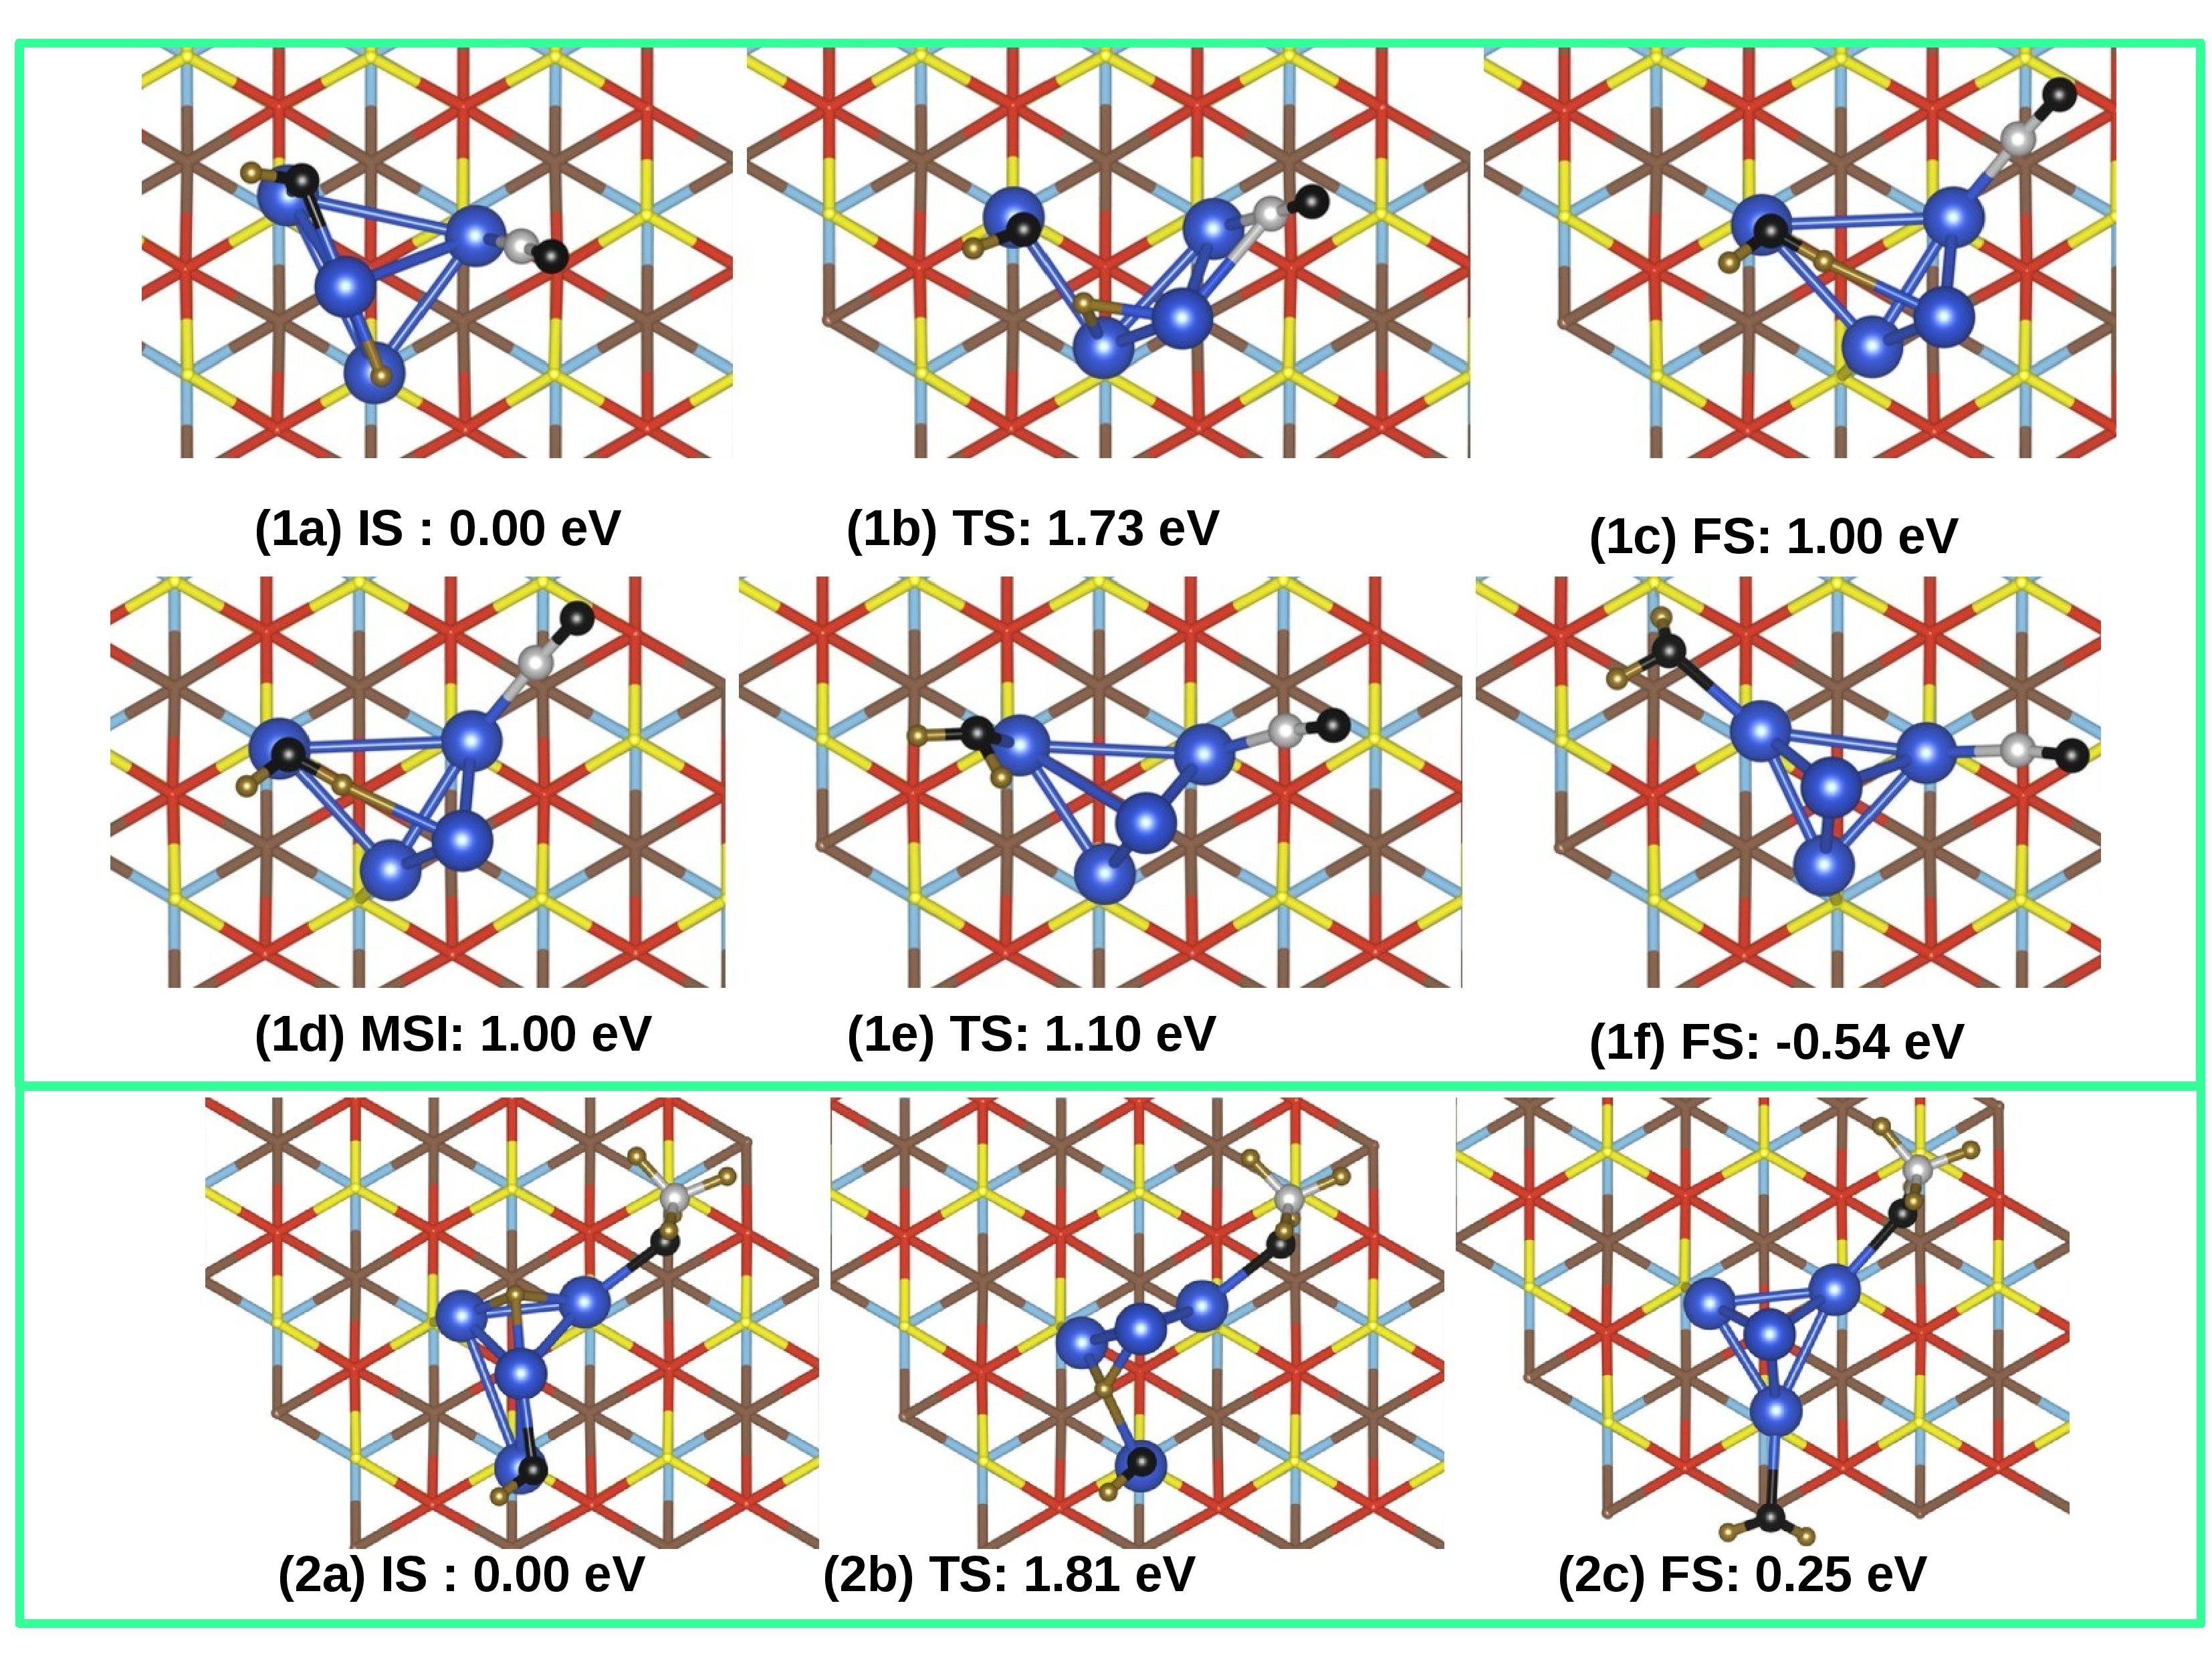
\includegraphics[width=0.9\textwidth]{./Appendix3/figures_si/p_120.jpg}
  \end{center}
    \caption{ Reaction in top (tetrahedron tetramer, 1a-1f) panel: *CO + *OH + *H $\rightarrow$ *CO + *H$_2$O. Reaction in bottom (tetrahedron tetramer, 2a-2c) panel: *CH$_3$OH + *OH + *H $\rightarrow$ *CH$_3$OH + *H$_2$O.  }
  \label{fig:si-119}
\end{figure}

%\begin{figure}
%  \begin{center}
%    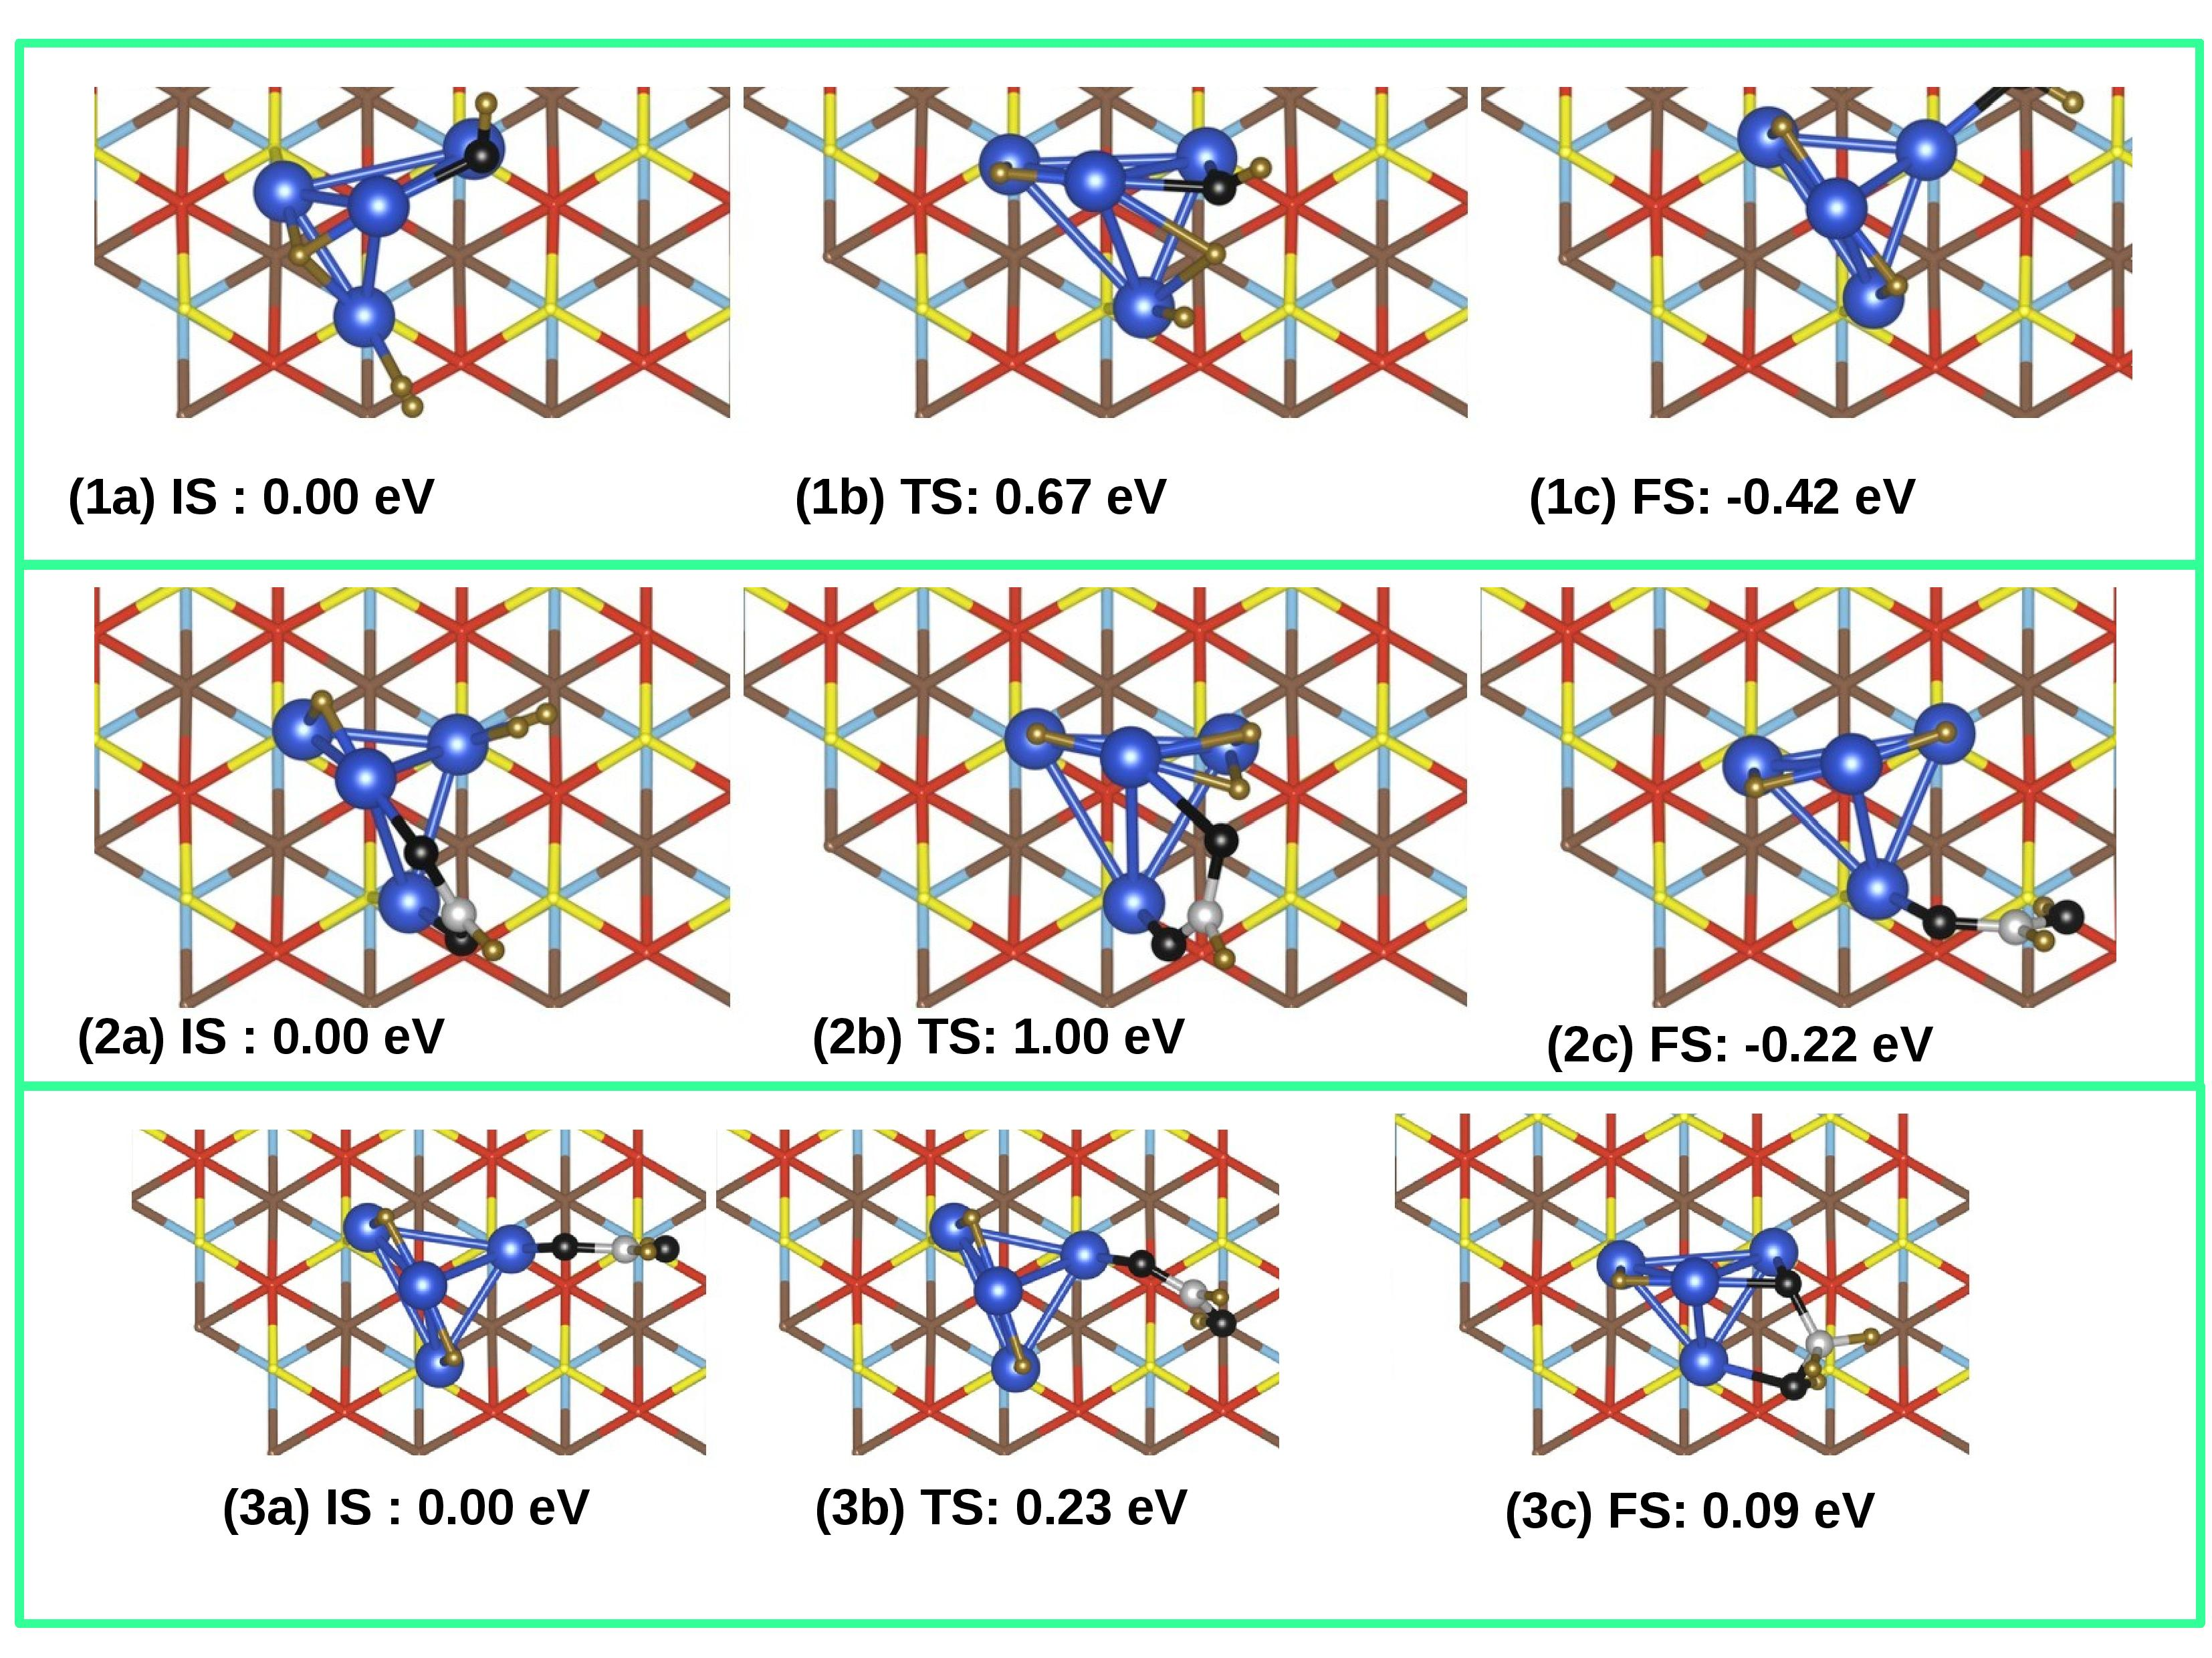
\includegraphics[width=0.9\textwidth]{./Appendix3/figures_si/p_121.jpg}
%  \end{center}
%    \caption{Reaction in top (tetrahedron tetramer, 1a-1c) panel: *OH + *H + *H$_2$ $\rightarrow$ *H$_2$O + *H + *H. Reaction in middle (tetrahedron tetramer, 2a-2c) panel: *HCOO + *H + *H$_2$ $\rightarrow$ *HCOOH + *H + *H. Reaction in bottom (tetrahedron tetramer, 3a-3c) panel: *HCOOH + *H + *H $\rightarrow$ *CH$_2$OOH + *H. }
%  \label{fig:si-120}
%\end{figure}

%\begin{figure}
%  \begin{center}
%    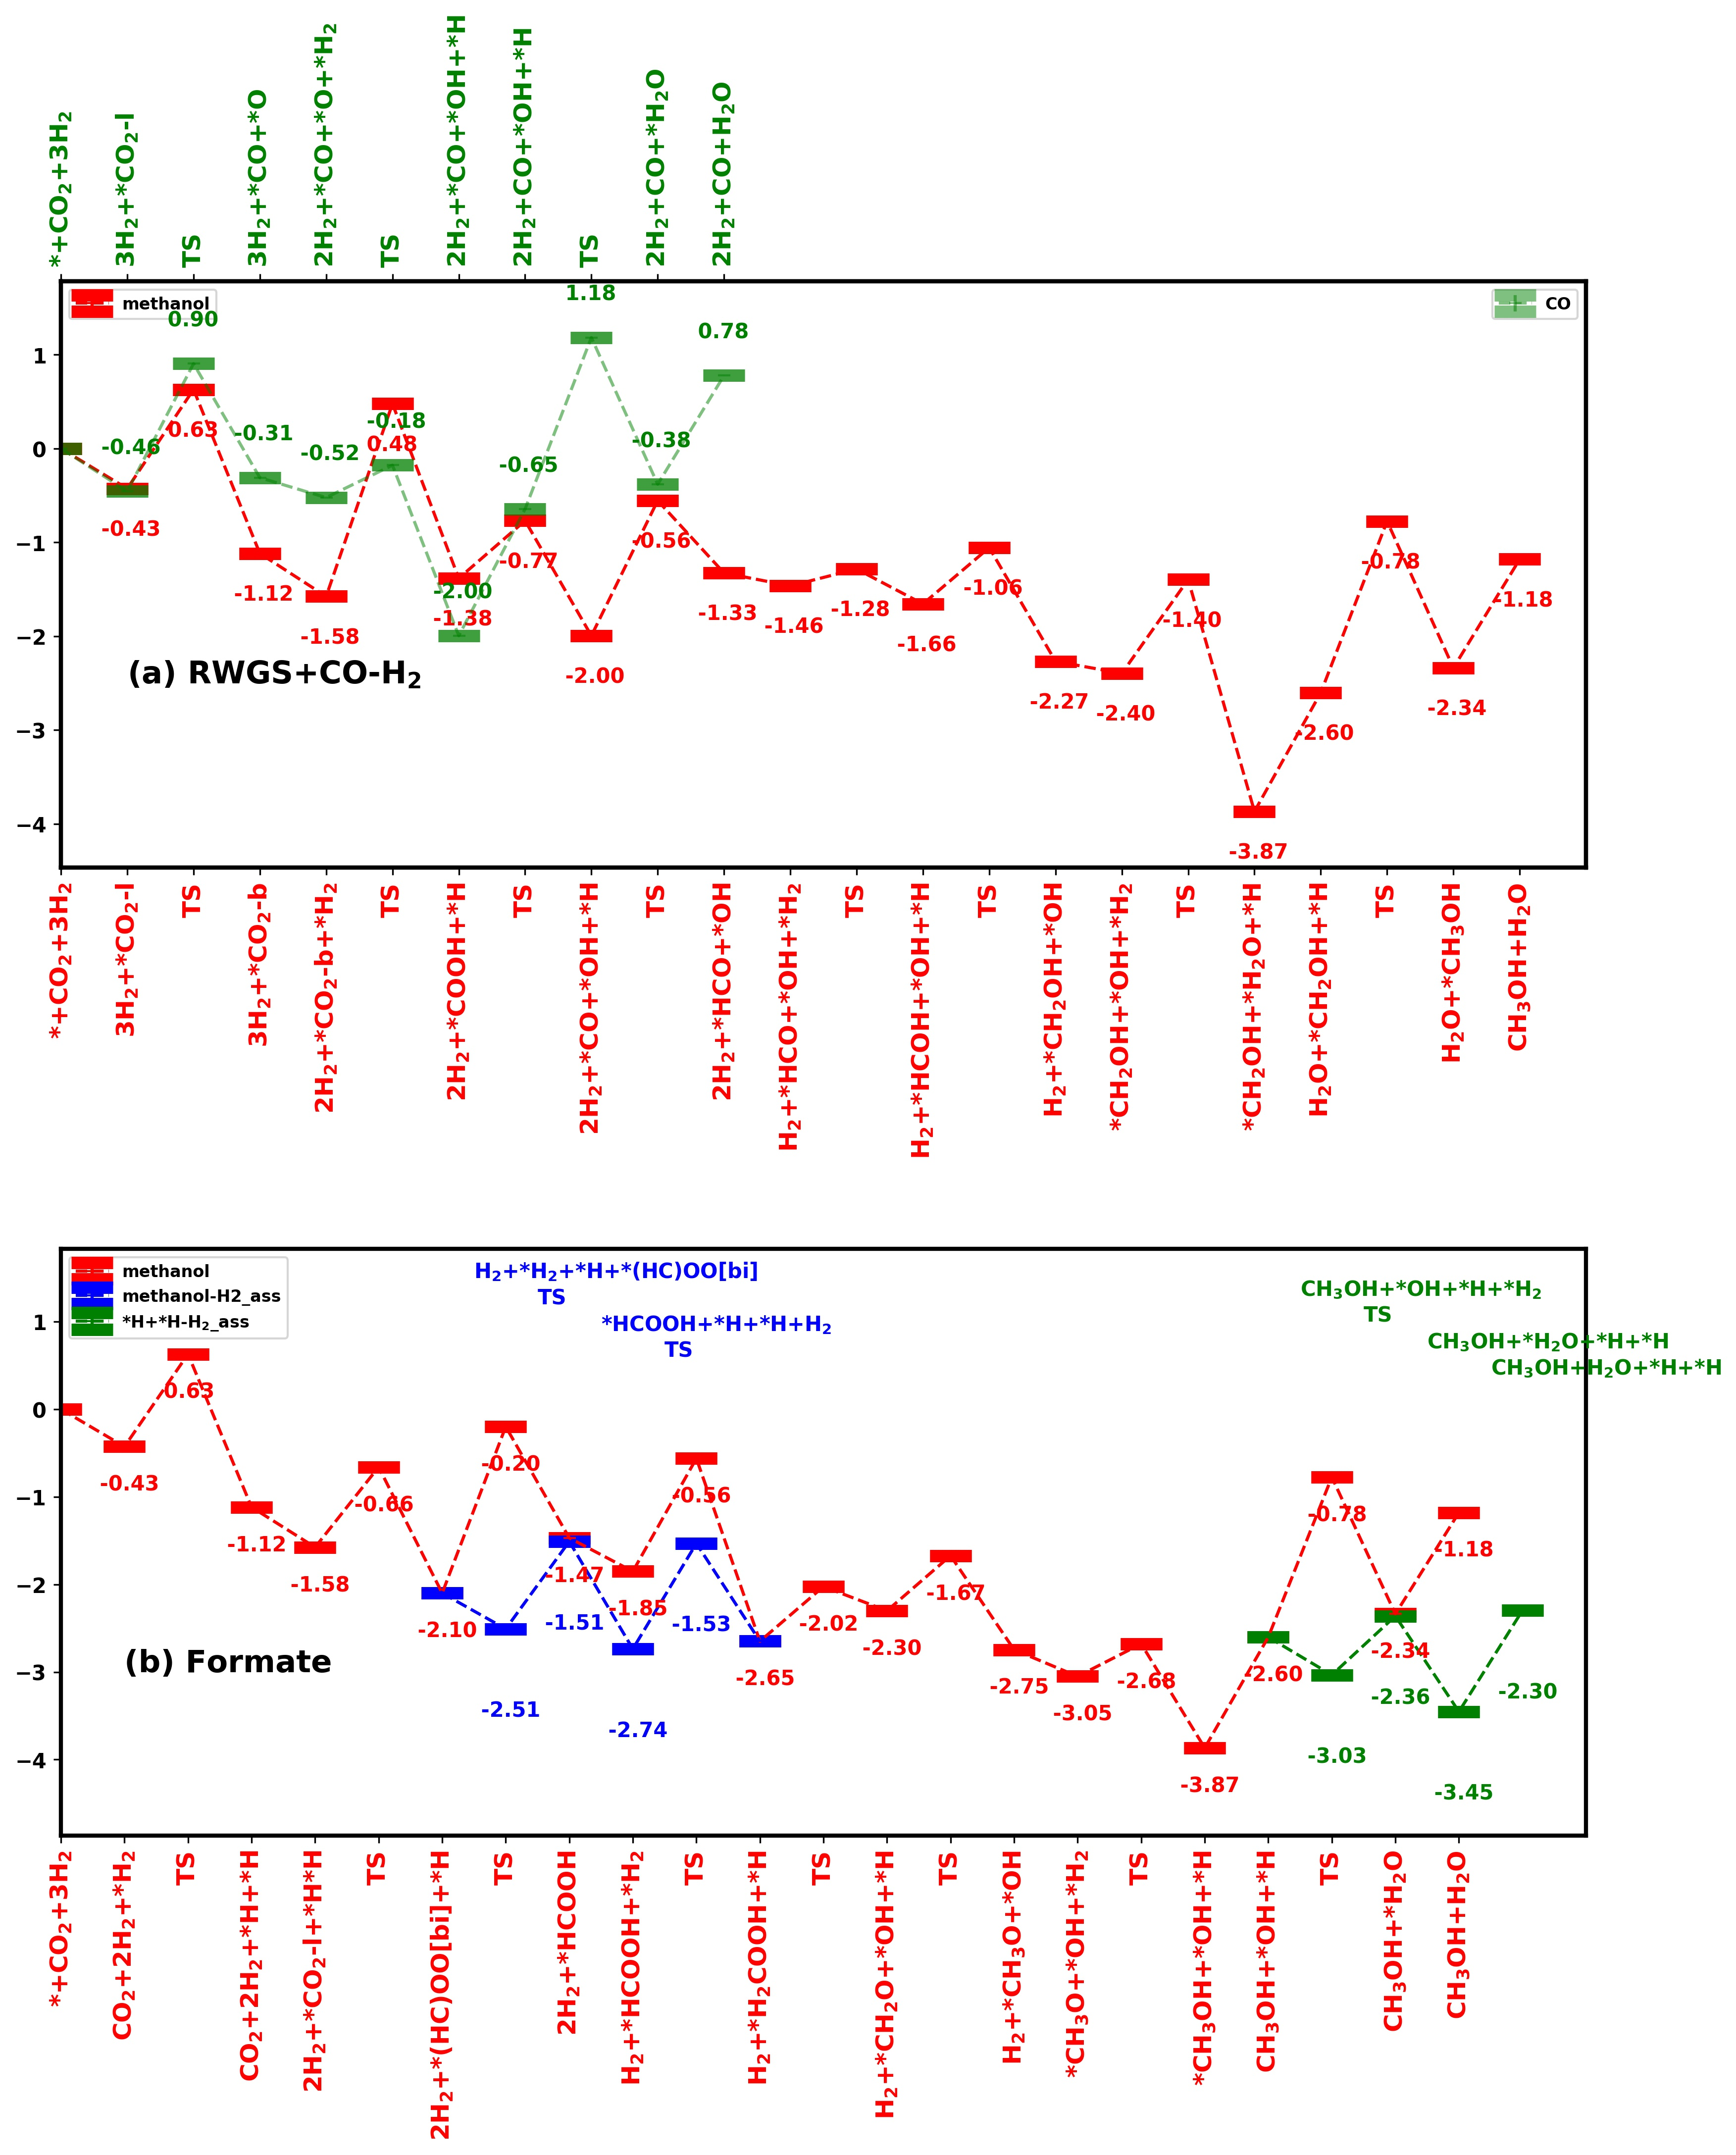
\includegraphics[width=0.9\textwidth]{./Appendix3/figures_si/p_122.jpg}
%  \end{center}
%    \caption{Reaction profile for the reduction of CO$_2$ on (a) rhombus and (b) tetrahedron tetramer supported on Ti$_2$CO$_2$. The most favourable (reported in Figure \ref{fig:05a} and \ref{fig:05b}) along with possible side reactions are provided here. }
%  \label{fig:si-121}
%\end{figure}


%\begin{figure}
%  \begin{center}
%    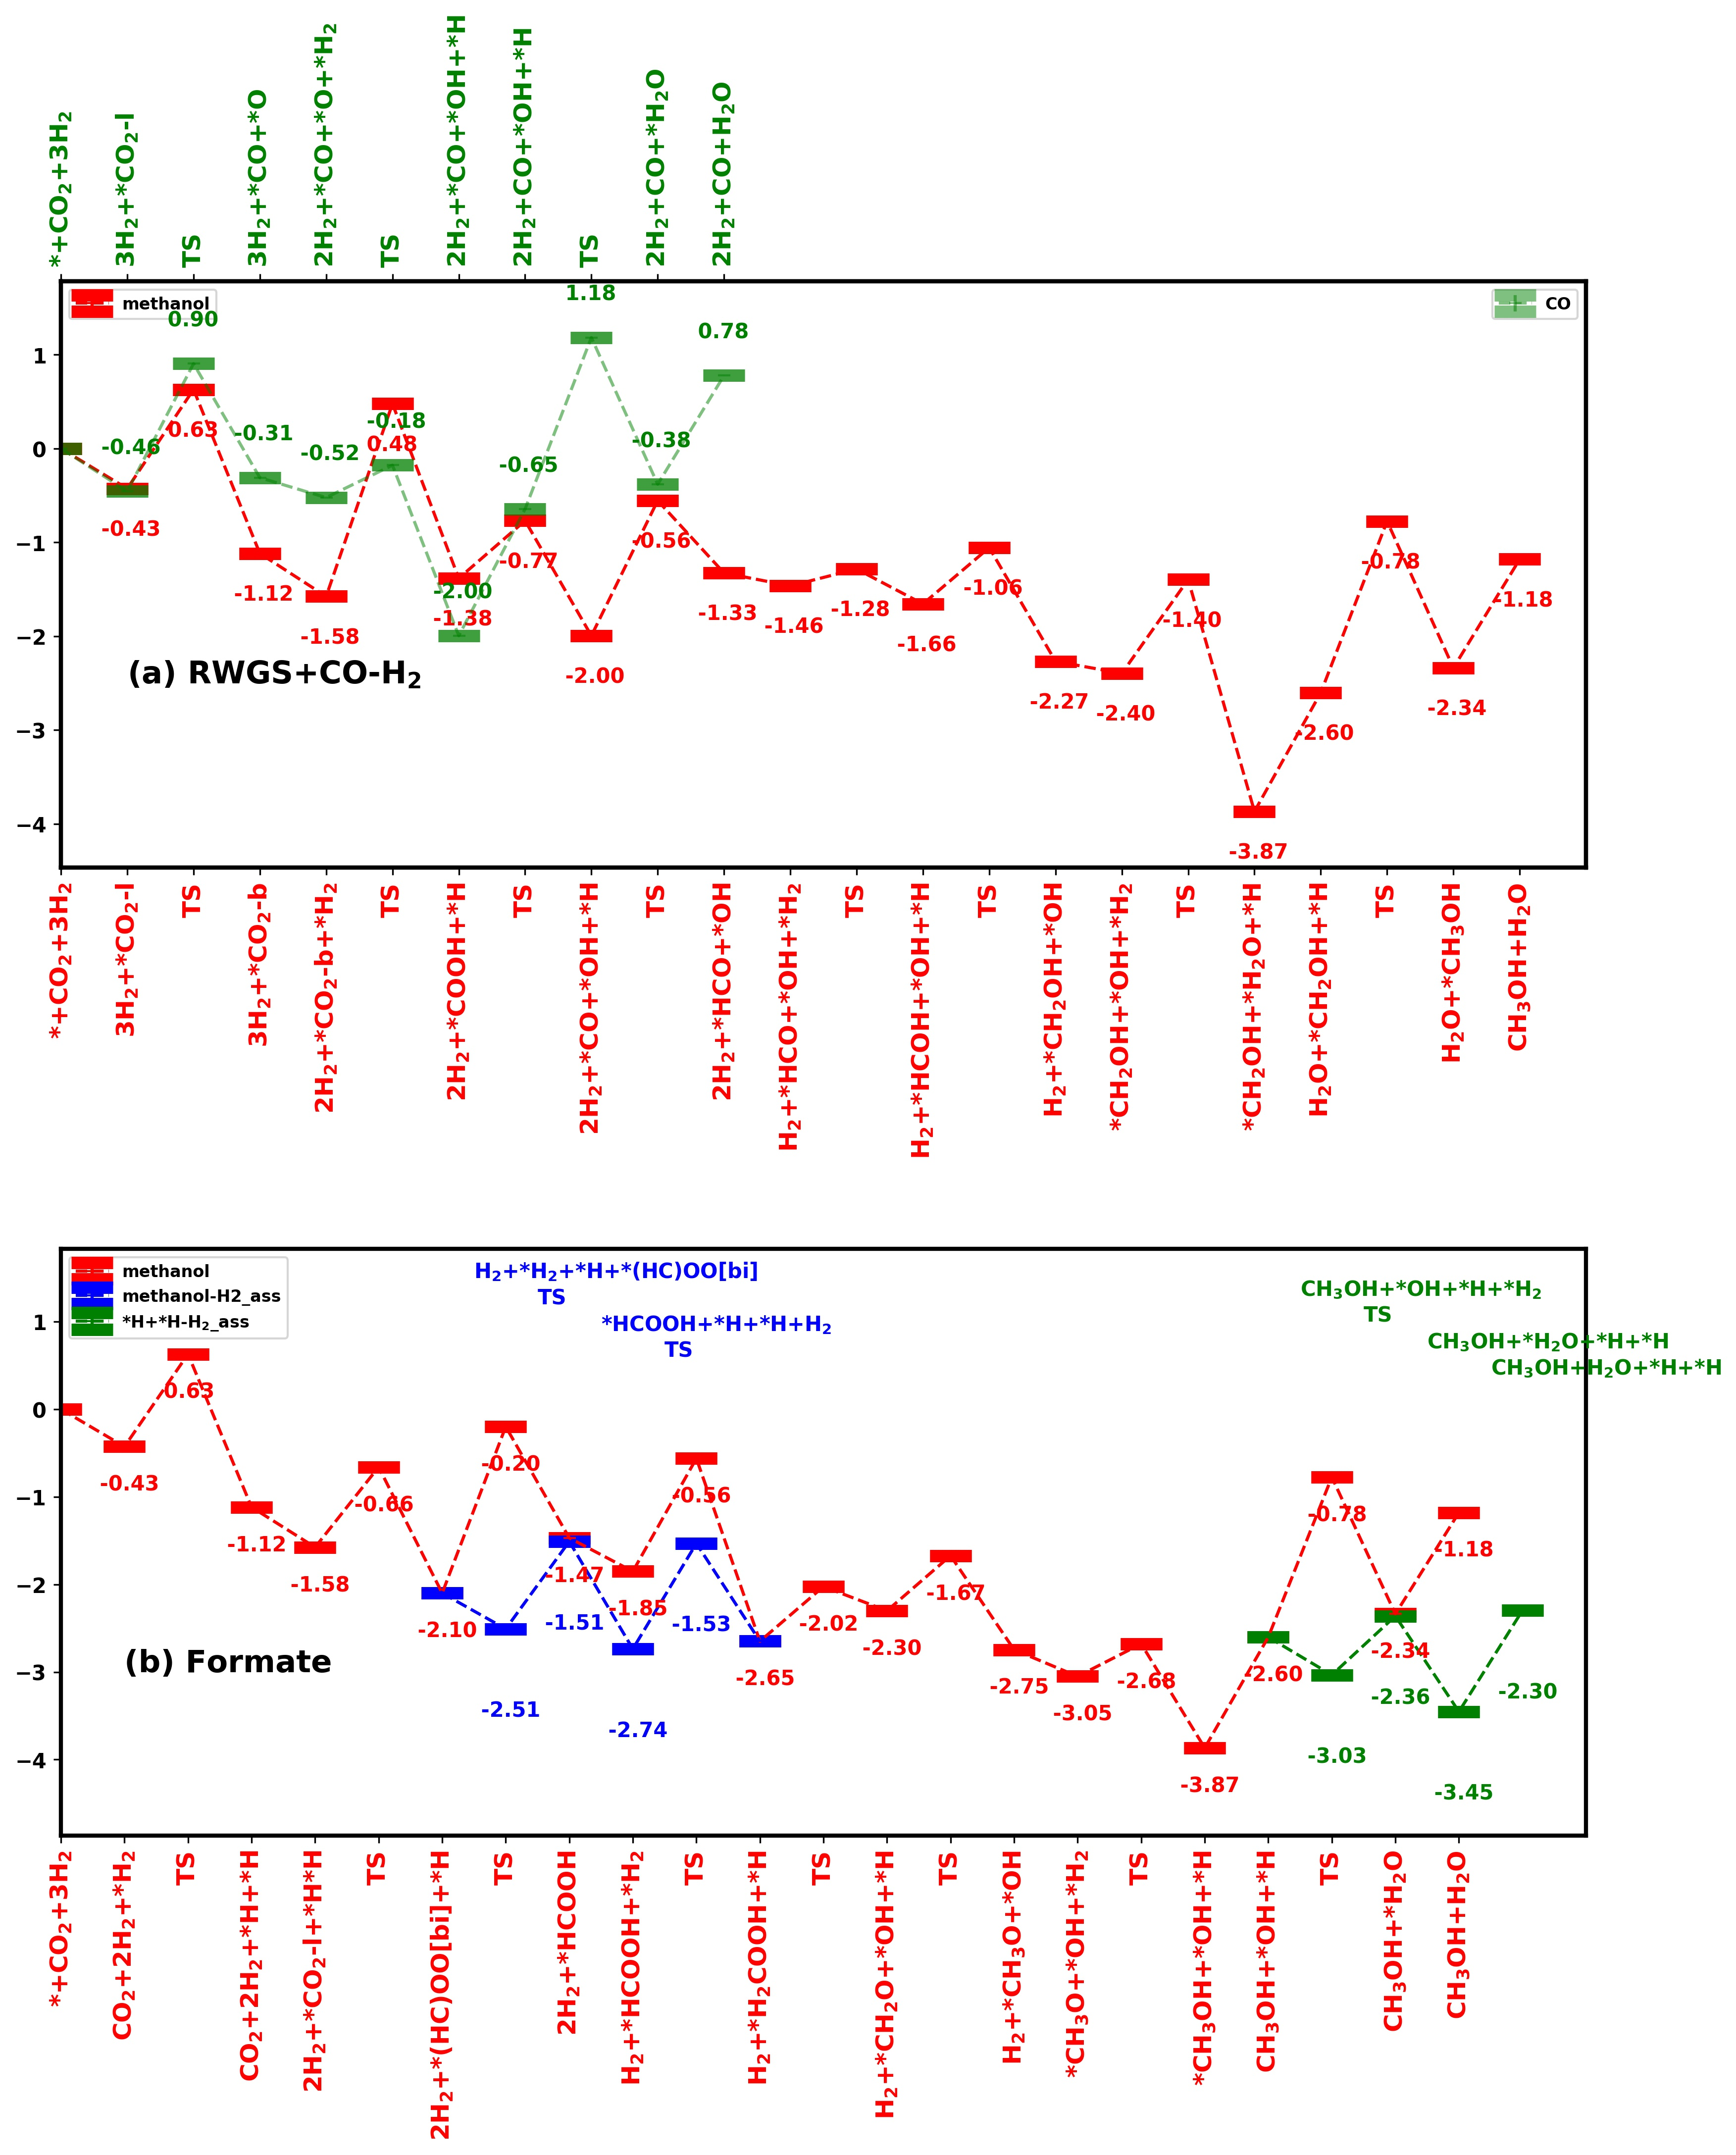
\includegraphics[width=0.9\textwidth]{./Appendix3/figures_si/p_122.jpg}
%  \end{center}
%    \caption{Equation:  }
%  \label{fig:si-122}
%\end{figure}







